\setchapterstyle{kao}
\setchapterpreamble[u]{\margintoc}

\chapter{Detecting Low Energetic Double Cascades}
\labch{double_cascade_performance}


\section{Reconstruction}

All existing reconstruction algorithms applied for low energetic atmospheric neutrino events mentioned in \refsec{reconstruction} are either assuming a single cascade hypothesis or a track and cascade hypothesis, which are the two SM morphologies observable at these energies, as was described in \refsec{icecube_signatures}. A HNL being produced and decaying inside the IceCube detector however, will produce two cascade like light depositions. The morphology and how the cascade properties and their spatial separation depend on the model parameters was introduced in \refsec{double_cascade_morphology}. To investigate the performance of the detector to observe these events, a low energetic double cascade reconstruction algorithm was developed, based on a pre-existing algorithm used to search for double cascades produced from high energetic astrophysical tau neutrinos \sidecite{Abbasi:2020zmr} that was established in \sidecite{MUsner}, but first mentioned in \sidecite{PHallen}.


\subsection{Table-Based Minimum Likelihood Algorithms}

The reconstruction is relying on a maximum likelihood algorithm, which is the \textit{classical} approach to IceCube event reconstructions, as opposed to ML based methods. A Poissonian likelihood is constructed, which compares the observed photon numbers, $n$, with their arrival times to the expected light depositions, $\mu$, for a given even hypothesis as\todo{maybe I want a figure for this, or not so important? (YELLOW)}
\begin{equation}
    \ln(L) = \sum_j \sum_t n_{j,t} \cdot \ln(\mu_{j,t}(\Theta) + \rho_{j,t}) - (\mu_{j,t}(\Theta) + \rho_{j,t}) - \ln(n_{j,t}!)
    \;,
    \labeq{millipede_likelihood}
\end{equation}
where $\rho$ are the number of expected photons from noise, $\Theta$ are the parameters governing the source hypothesis, and the likelihood is calculated summing over all DOMs $j$ splitting observed photons into time bins $t$. The light expectations are calculated using look-up tables \sidecite{photospline} that contain the results from MC simulations of reference cascade events or track segments. By varying the parameters defining the event hypothesis, the likelihood of describing the observed light pattern by the expected light depositions is maximized to find the reconstructed event. Algorithms of this kind used in IceCube are described in great detail in \sidecite{IceCube:2013dkx}. For the table production a specific choice of ice model has to be made, while the calibrated DOM information is taken from the measurement itself.

% \subsection{Double Cascade Hypothesis}

Based on the tabulated light expectations for cascades and track segments, various event hypothesis can be constructed, like the common cascade only or the track and cascade hypotheses. The hypothesis describing the double cascade signature of the HNL is using two reference cascades that are separated by a certain distance. The whole hypothesis is defined by 9 parameters and assumes that the two cascades are aligned with each other, which is a safe assumption for strongly forward boosted interactions\todo{Elaborate whether this is the case (show it in a plot?). Discuss directionality of cascades in general. (ORANGE)}. The parameters are the position of the first cascade $x, y, z$, the direction of both cascades $\phi, \theta$, and its time $t$ as well as the decay length $L$ between the two cascades. Assuming the speed of the HNL to be the speed of light, $c$, this already defines the full signature. The HNL particle does not produce any light while traveling, as it is electrically neutral. The full 9 parameters describing the event are $\Theta = (x, y, z, t, \theta, \phi, E_0, E_1, L)$. To compute the full likelihood the term in \refeq{millipede_likelihood} is summed over both cascade parts, $i$, as $\sum_i \ln(L_i)$. 


\subsection{Optimization for Low Energy Events}

Optimizing the double cascade reconstruction for low energetic events was done in parallel to the development of the model dependent simulation generator introduced in \refsec{model_specific_simulation}. A preliminary sample of HNL events was used, containing a continuum of masses between \SIrange[range-phrase=~and~]{0.1}{1.0}{\gev} and lab frame decay lengths sampled uniformly in the range from \SIrange{5}{500}{\meter}. Even though this sample is not representative of a physically correct model and therefore not useful to predict the event expectation, it can still be used to optimize the reconstruction. The double cascade nature of the individual events and the evenly spaced decay length distribution are especially useful for this purpose.

The simulation is processed up to Level 5 of the selection chain described in \refsec{event_selection} and one of the reconstructions from \sidecite{low_energy_reco_IC} is applied to the events, fitting a cascade and a track and cascade hypothesis. The results from this reconstruction are used as an input for the double cascade reconstruction, where the position of the vertex, the direction of the event, and its interaction time are used as the input quantities for the first cascade, and the length of the track reconstruction is used as a seed for the distance between the two cascades.


\subsubsection{Decay Length Seeds}

\begin{figure*}[h]
	\centering
    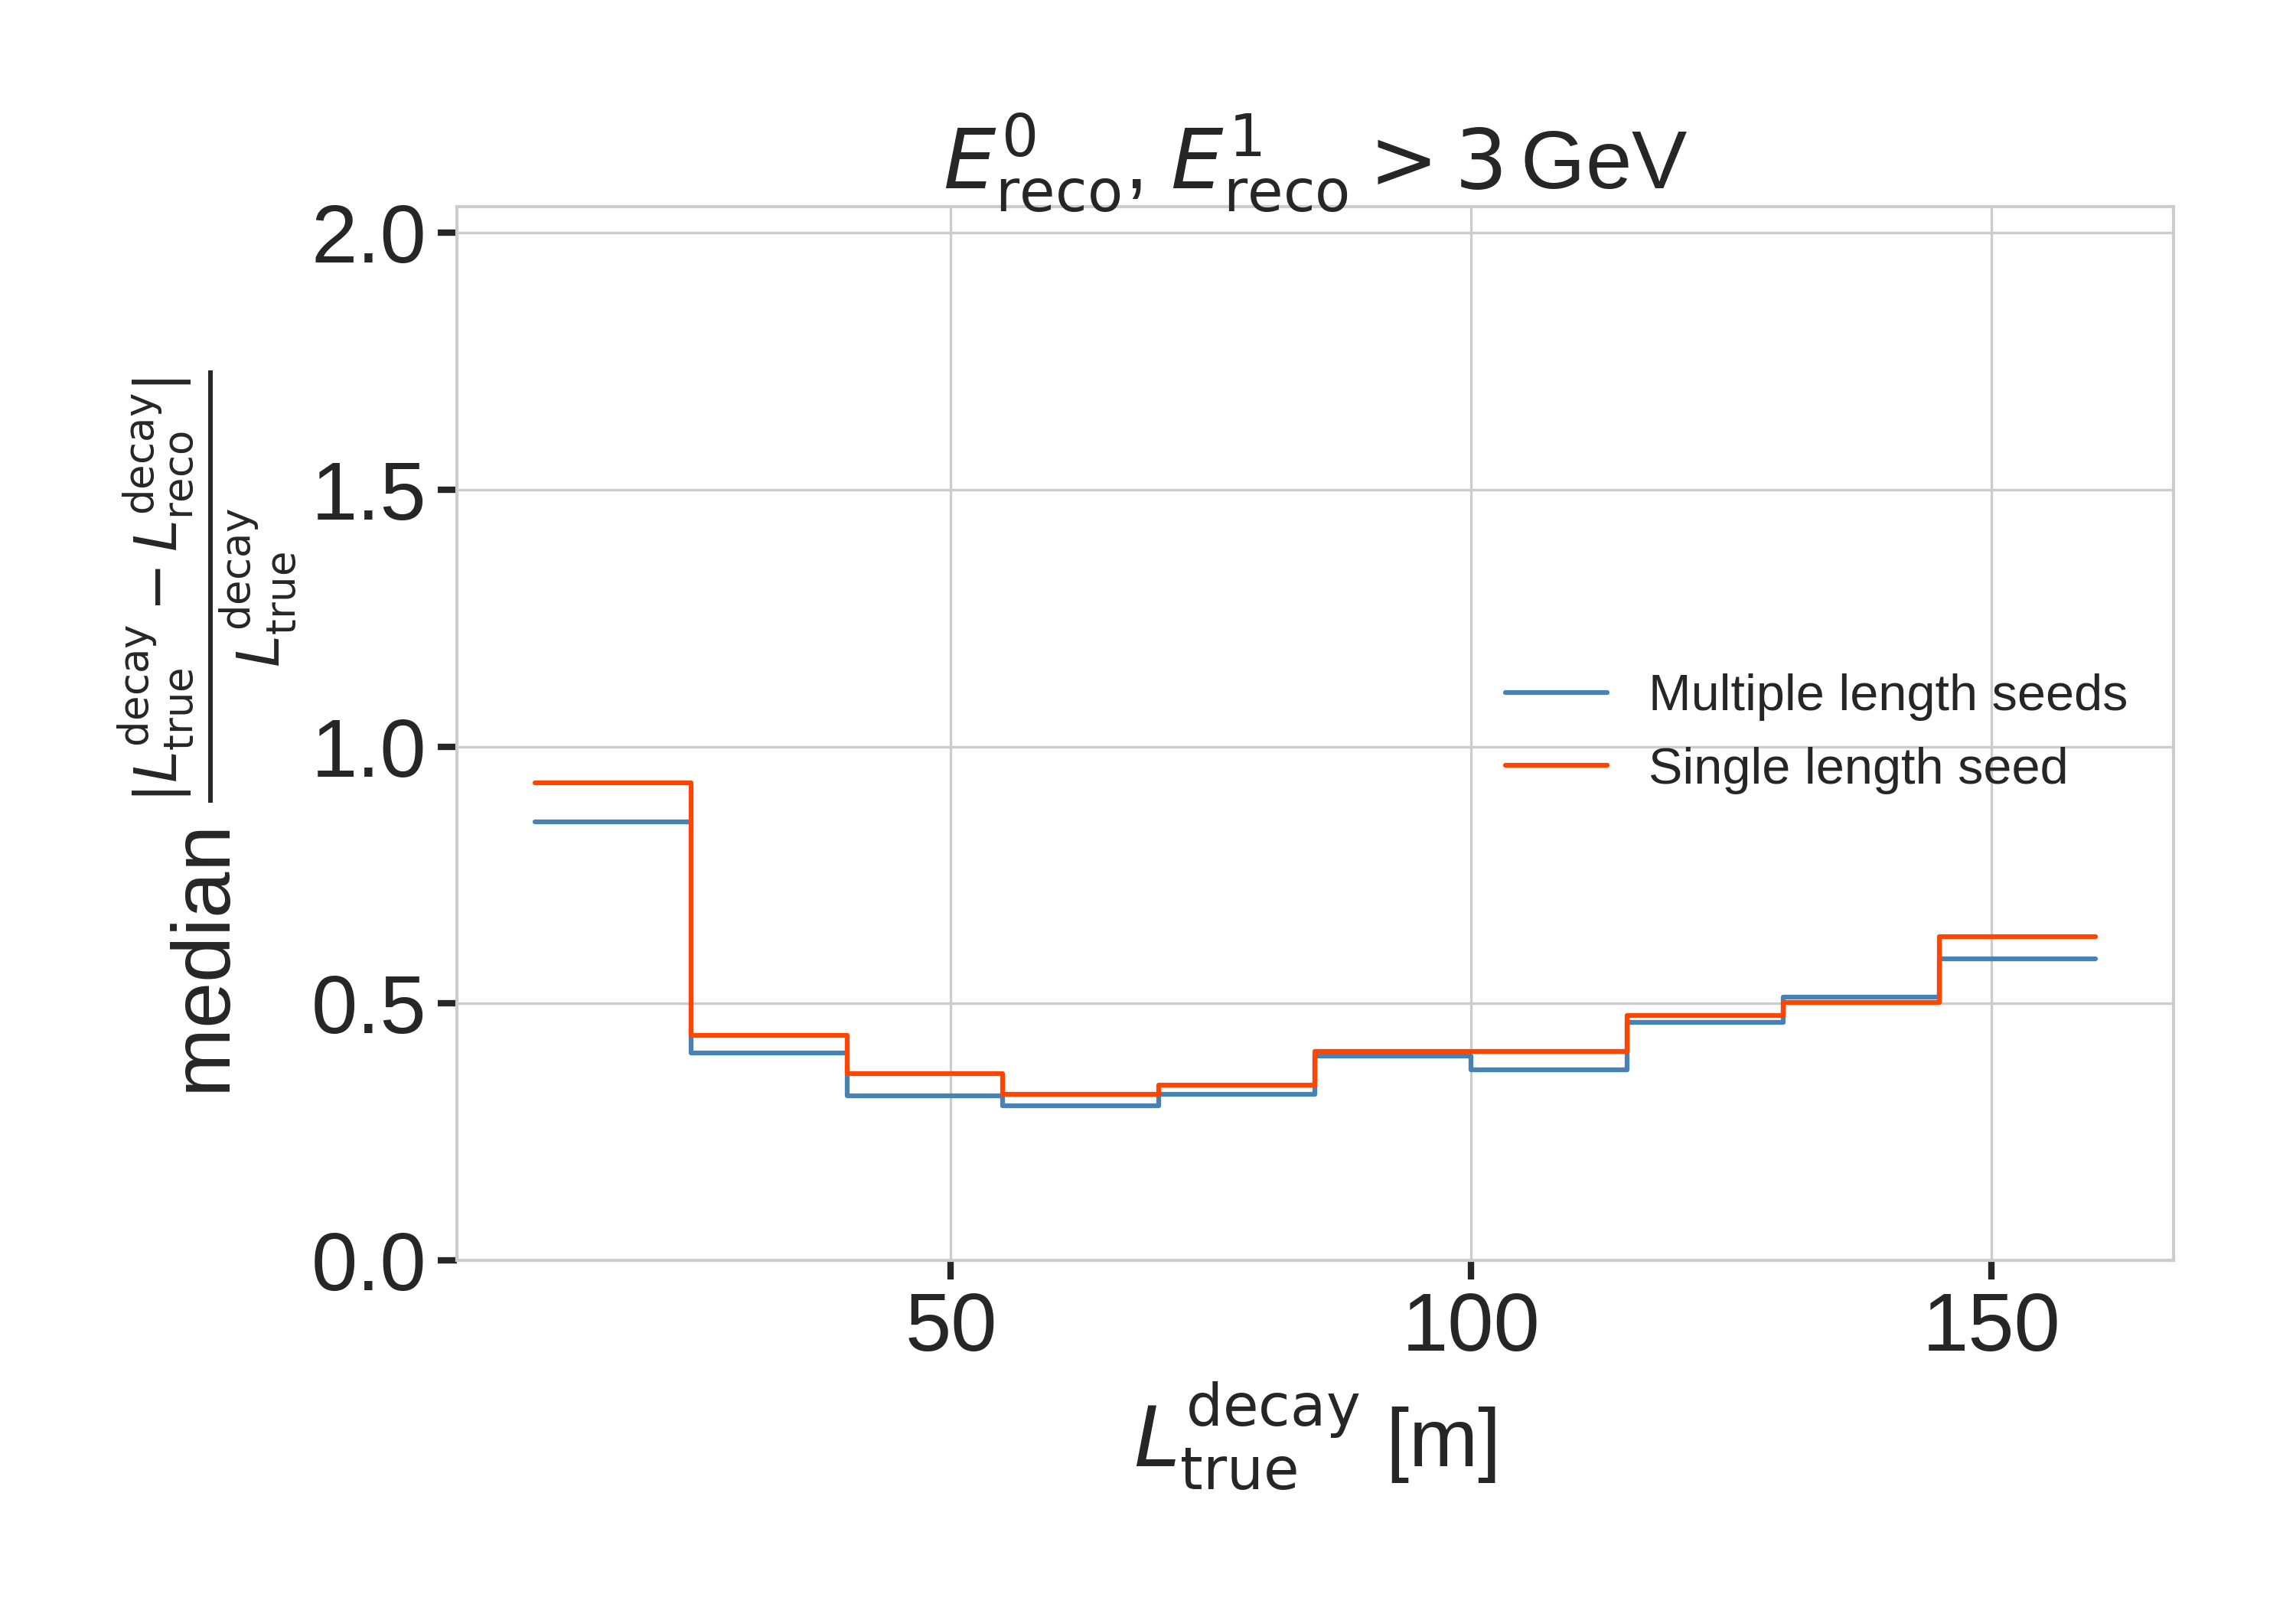
\includegraphics[width=0.49\linewidth]{figures/results/190605_reco_optimization/decay_length_seeding_median_decay_length_resolution_Good + L7 + reco E1,E2 above 3_fix_y.png}
    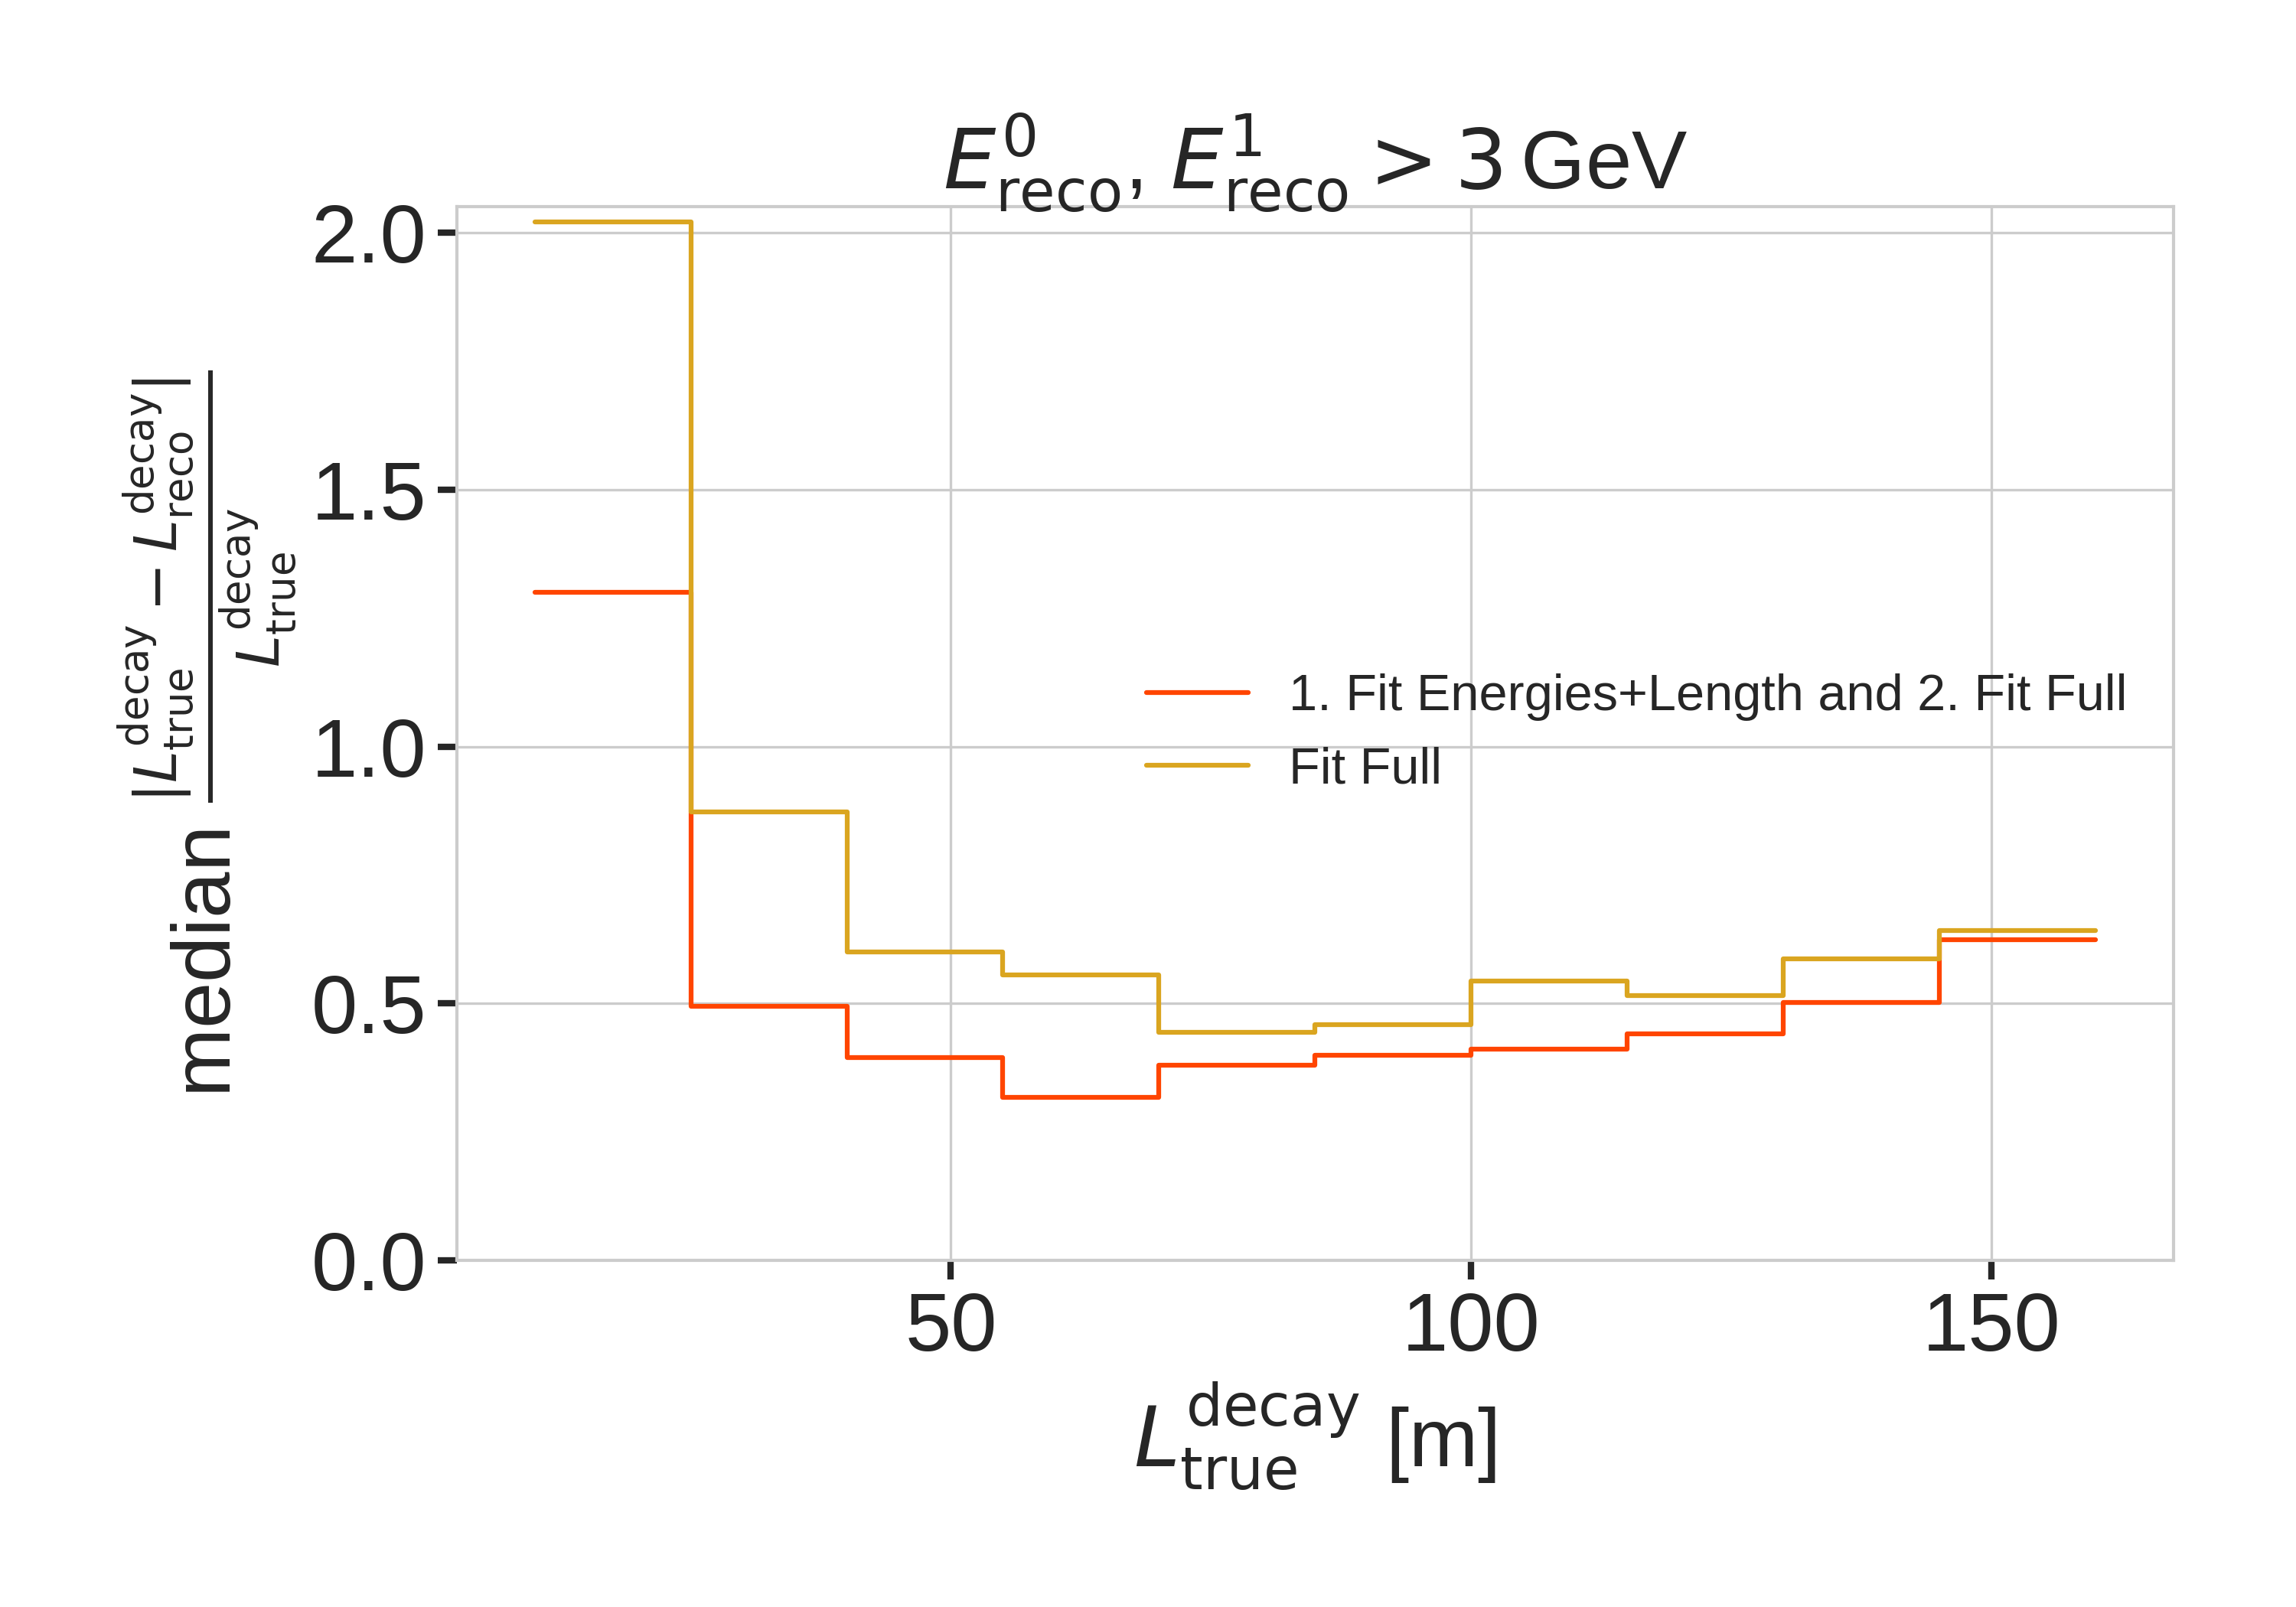
\includegraphics[width=0.49\linewidth]{figures/results/190605_reco_optimization/fit_routine_splitting_median_decay_length_resolution_Good + L7 + reco E1,E2 above 3_fix_y.png}
    \caption[]{}
    % \caption{Decay length resolution versus true decay length comparing the same fit routine seeded with just the seed decay length (Single length seed) and seeded with a decay length of 5\,m, 25\,m, 50\,m, 100\,m, and 200\,m (Multiple length seeds). This was done with older signal simulation sample (190605) and the resolution is unweighted.}
    % \caption{Decay length resolution versus true decay length comparing a full 9 paramters fit to an iterative approach where first the energies and the decay lenght are fitted, while fixing the other 7 parameters and then the full fit is performed. This was done with older signal simulation sample (190605) and the resolution is unweighted.}
    \labfig{fit_routine_optimization}
\end{figure*}
\todo{fix caption of this figure (RED)}

The full 9 dimensional likelihood space is very complex and can have many local minima, depending on the specific event and its location in the detector. Especially the seed value of the length between the two cascades was found to have a very strong impact on whether the global minimum was found during the minimization. To mitigate this effect, multiple fits are performed, seeding with variations of the input length at different orders of magnitude. The best result is used, selected based on the total likelihood value of the best fit parameter set. A small improvement in the decay length resolution can be found by using this approach as compared to a single length seed. The effect can be seen in the left part of \reffig{fit_routine_optimization}, which shows the median, absolute, fractional decay length resolution.


\subsubsection{Fit Routine}

Because the length seed showed to have such a large impact on the reconstruction performance, a more sophisticated fit routine, than just fitting all 9 parameters at once, was tested. In a first fit iteration, some parameters are fixed and the resulting best fit point is used to fit all 9 parameters in a second iteration. In the right part of \reffig{fit_routine_optimization} it can be seen how a fit split into two consecutive steps, where the first step fits only both cascade energies and the decay length and the second step fits the full 9 parameters, performs better as compared to a single, full 9 parameter fit. The initial seed for both routines is the same.


\subsubsection{Minimizer Settings}

To investigate the effect of the minimizer used to find the best fit parameters, the reconstruction was performed using three different minimizers, which were easily accessible within the reconstruction framework. The minimizers used were Minuit1 Simplex, Minuit2 Simplex, and Minuit2 Migrad. The results can be seen in \reffig{minimizer_optimization}, where the Minuit1 Simplex minimizer performs best. The initial idea was to test a global minimizer, or a routine that can find the rough position of the global minimum first and then a local minimizer to find the exact minimum, but unfortunately this was not possible with the minimizers available in the framework. From the three tested minimizers, Minuit1 Simplex performed best and was chosen as the default for the reconstruction. The comparison of the decay length resolutions can be seen in \reffig{minimizer_optimization}.


\begin{figure}[h]
    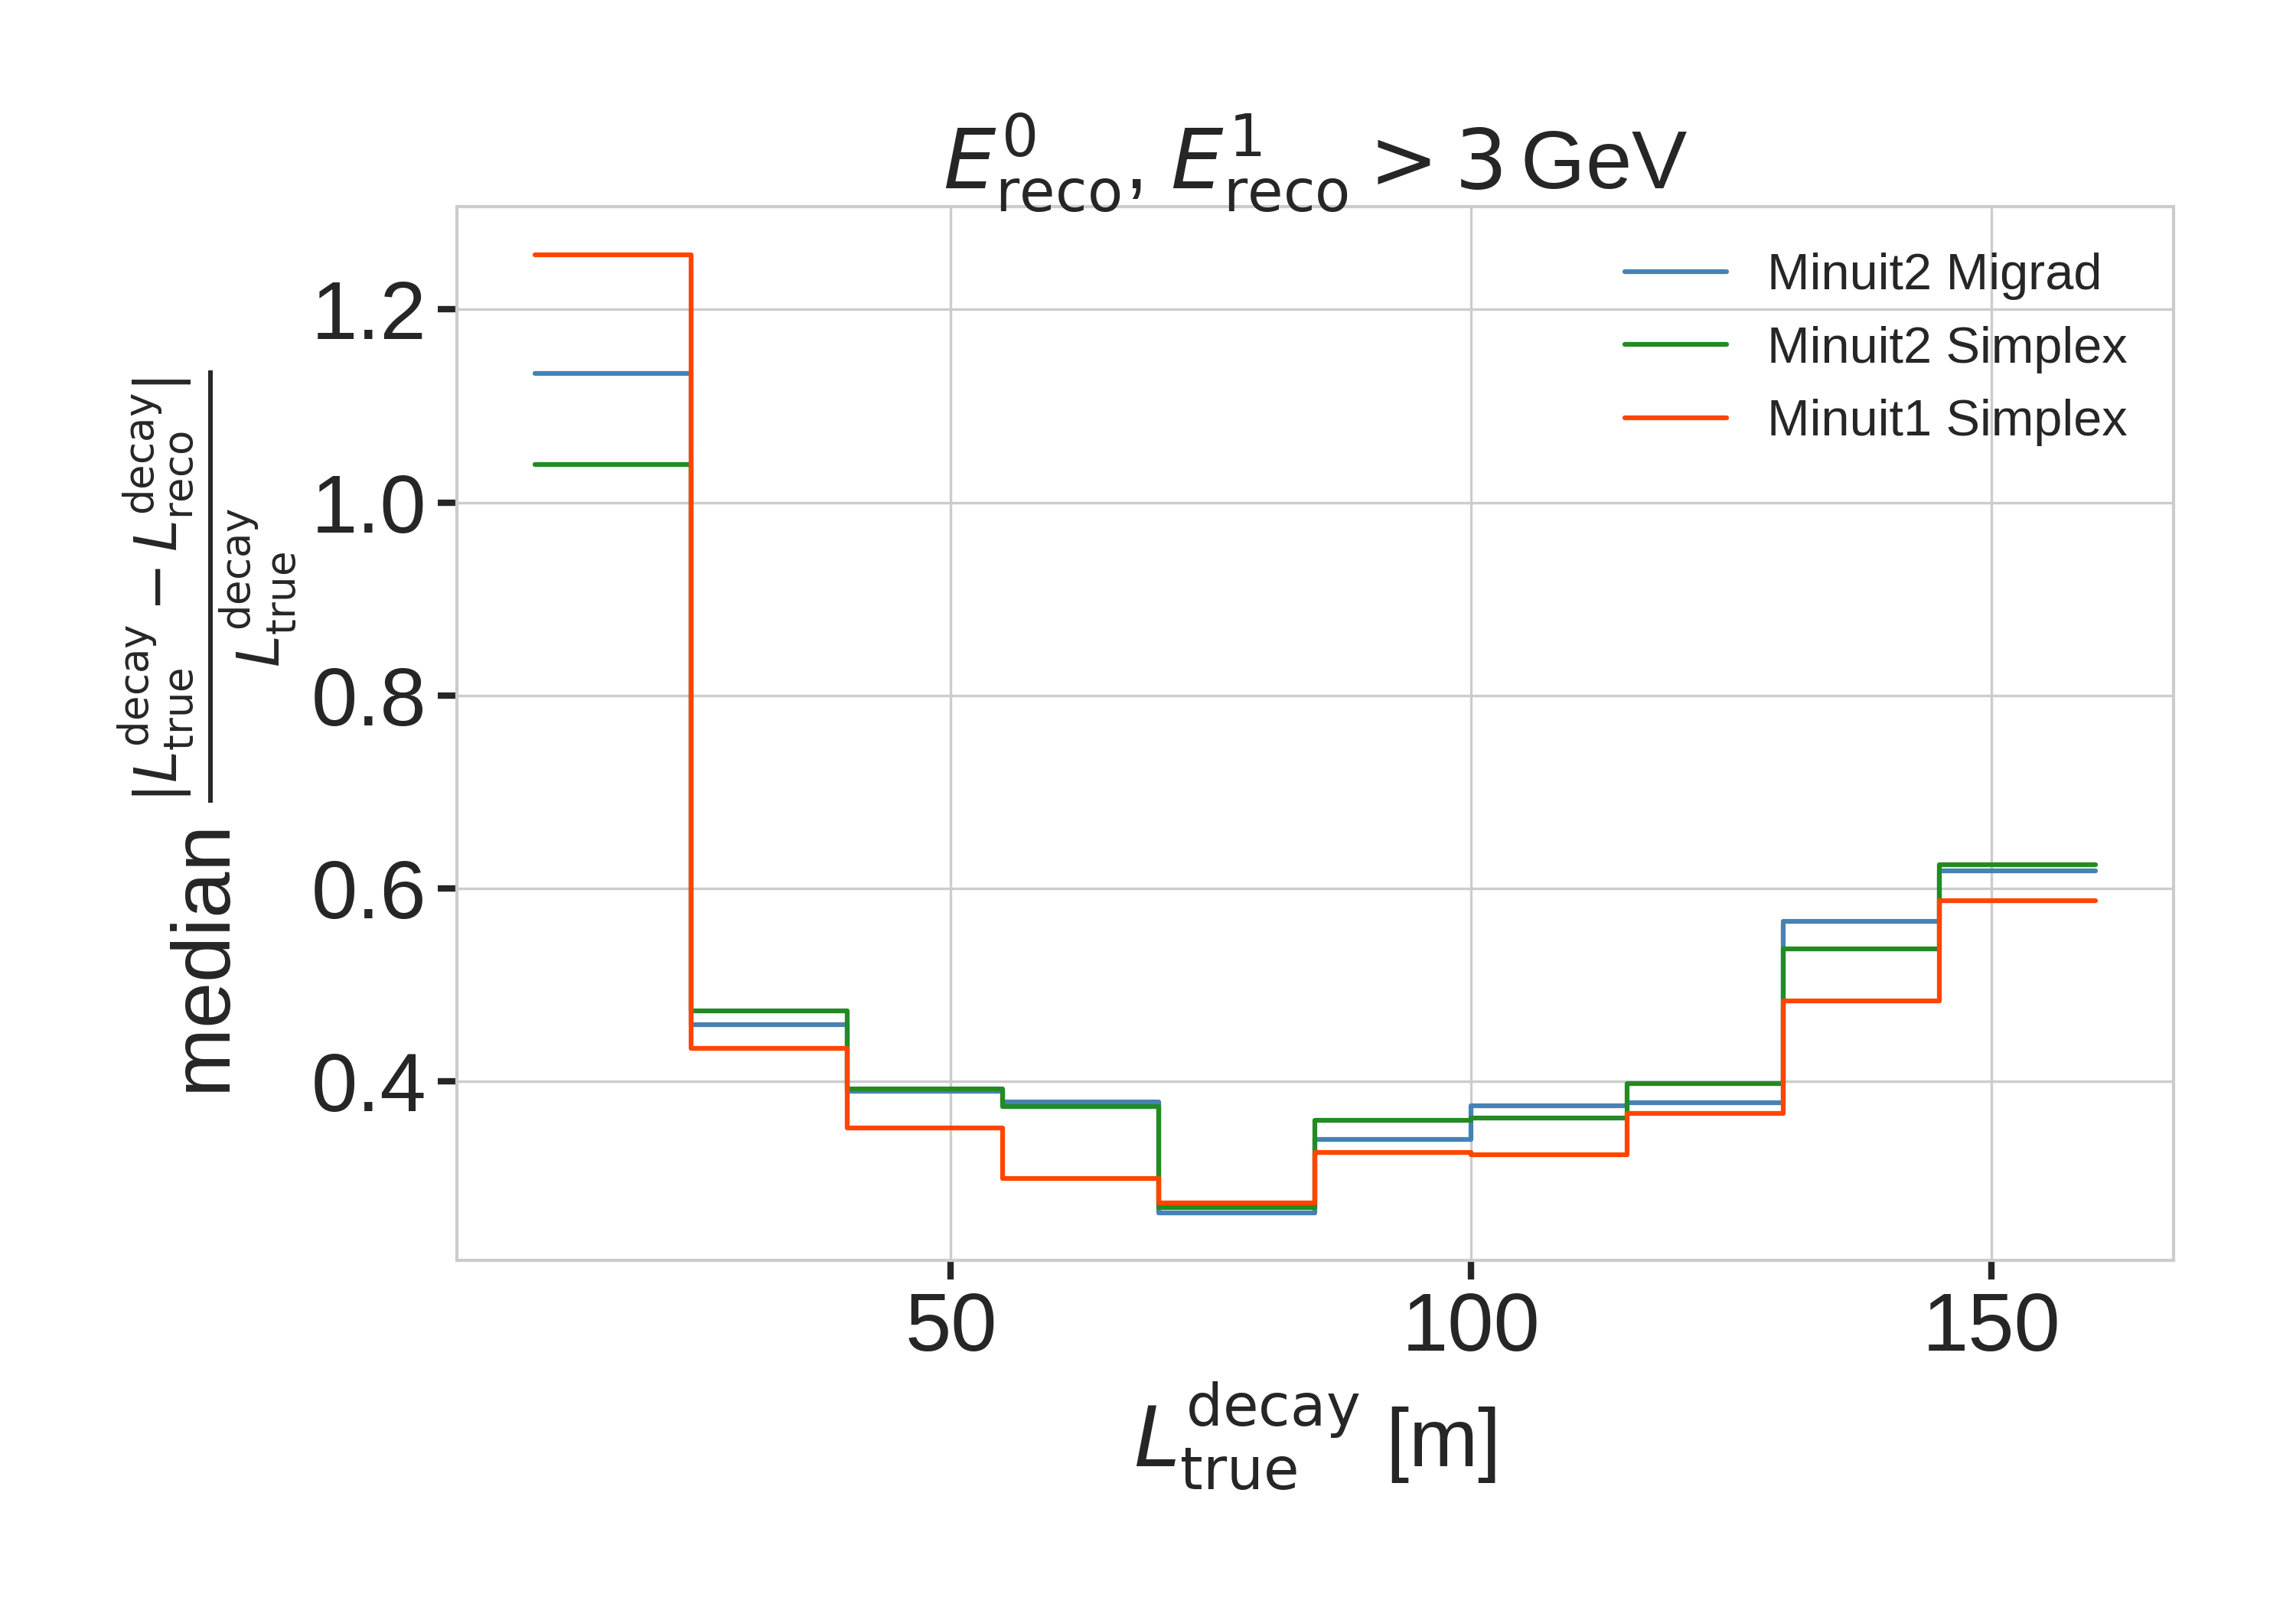
\includegraphics{figures/results/190605_reco_optimization/minimizer_checks_median_decay_length_resolution_Good + L7 + reco E1,E2 above 3.png}
    \caption[short]{title}
    % \caption{Decay length resolution versus true decay length comparing the same fit routine performed with a different minimizer. These are the minimizers accessible with the Millipede framework. The (obvious) settings were chosen to be the same, but there might still be some hidden differences explaining the discrepency between the Minuit1 and Minuit2 implementation of Simplex. This was done with older signal simulation sample (190605) and the resolution is unweighted.}
    \labfig{minimizer_optimization}
\end{figure}
\todo{fix caption of this figure (RED)}


\subsection{Performance}

The chosen reconstruction chain used to test the performance of the detector to observe low energetic double cascades is the following; Minuit1 Simplex is used as the minimizer, the decay length is seeded with 3 different values, 0.5x, 1.0x, and 1.5x the length of the track reconstruction, and the fit routine is split into two steps, where the first step fits the energies and the decay length and the second step fits the full 9 parameters. In the first step, the number of time bins in \refeq{millipede_likelihood} is set to 1, so just the number of photons and their spatial information is used. The second step is seeded with the best results from the first fit and here the number of time bins is chosen such that each photon falls into a separate time bin, which means all time information is used. The average runtime per event is $\sim$\SI{16}{\second} on a single CPU core, but is very dependent on the number of photons observed in the event, since the likelihood calculation in the second step scales with this number and a table lookup has to be performed for each photon.

To get a more realistic estimate of the reconstruction performance, it is run on a second preliminary sample of HNL events, containing masses between \SIrange[range-phrase=~and~]{0.1}{3.0}{\gev} and the lab frame decay length is sampled from an inverse distribution in the range from \SIrange{1}{1000}{\meter}, which is a better approximation of the expected exponential decay distribution of the HNL. The performance is shown for events where the reconstruction chain was successfully run, the event selection criteria up to level 7 are fulfilled, and the reconstructed energy of both cascades is above \SI{3.0}{\gev}\todo{one half sentence on why this number was chosen? (ORANGE)}. This is done to only investigate well reconstructed events with two significant light depositions at a usual final selection level of the oscillation analyses.


\subsubsection{Energy Resolutions} \labsec{190607_energy_resolutions}

The energy resolution is inspected by looking at the 2-dimensional distribution of reconstructed energy versus the true energy as shown in \reffig{selected_routine_2d_energy_results}. The bin entries are shown as well as the median and $\pm$\SI{25}{\percent} calculated per vertical column, to get an idea of the distribution for a given energy slice. The color scale is showing the PDF along in each true energy slice, which is the full information combined into the median$\pm$\SI{25}{\percent} lines. The reconstructed energy is only the energy that is observable from photons, while the true energy is the total cascade energy, including the parts that go into EM neutral particles that do not produce light. It is therefore not expected that the median lines up with the axis diagonal, but rather the reconstructed energy is going to be lower.

\begin{figure*}[h]
	\centering
    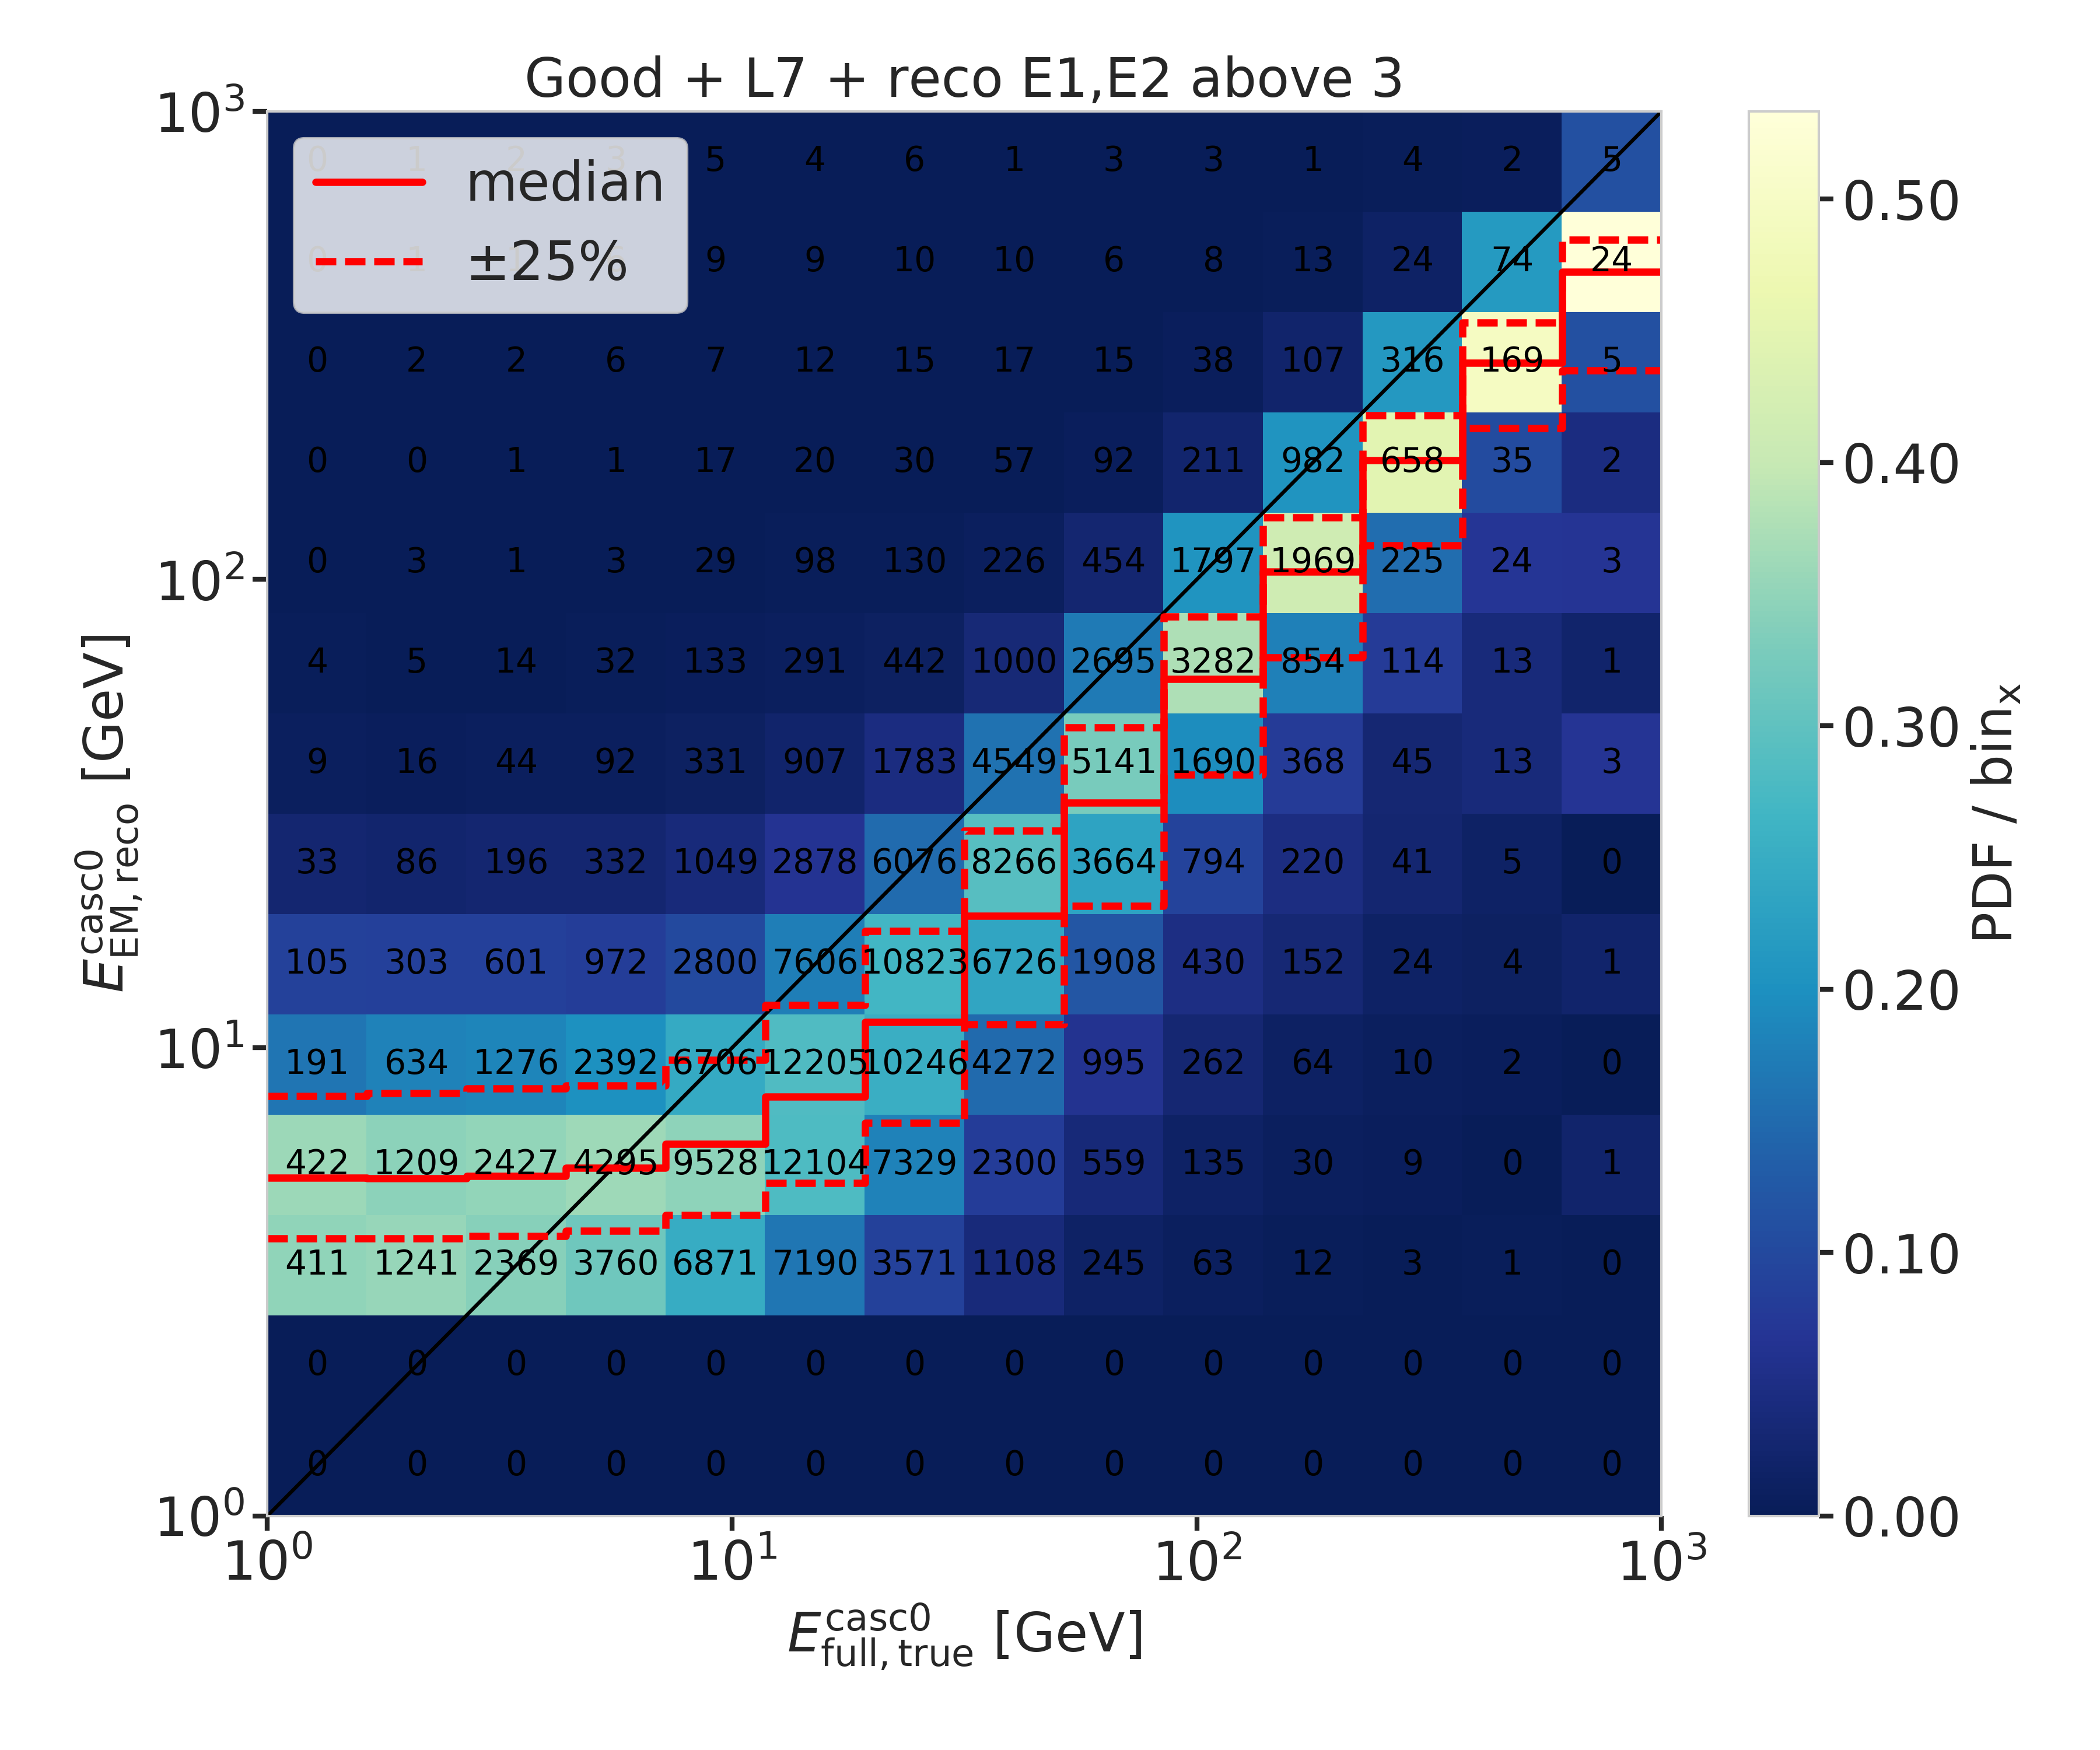
\includegraphics[width=0.49\linewidth]{figures/results/190607/resolutions/190607_millipede_level_no_NaNs_NEW_flipped_casc0_reco_energy_vs_casc0_true_energy_reco_above3_step_contours.png}
    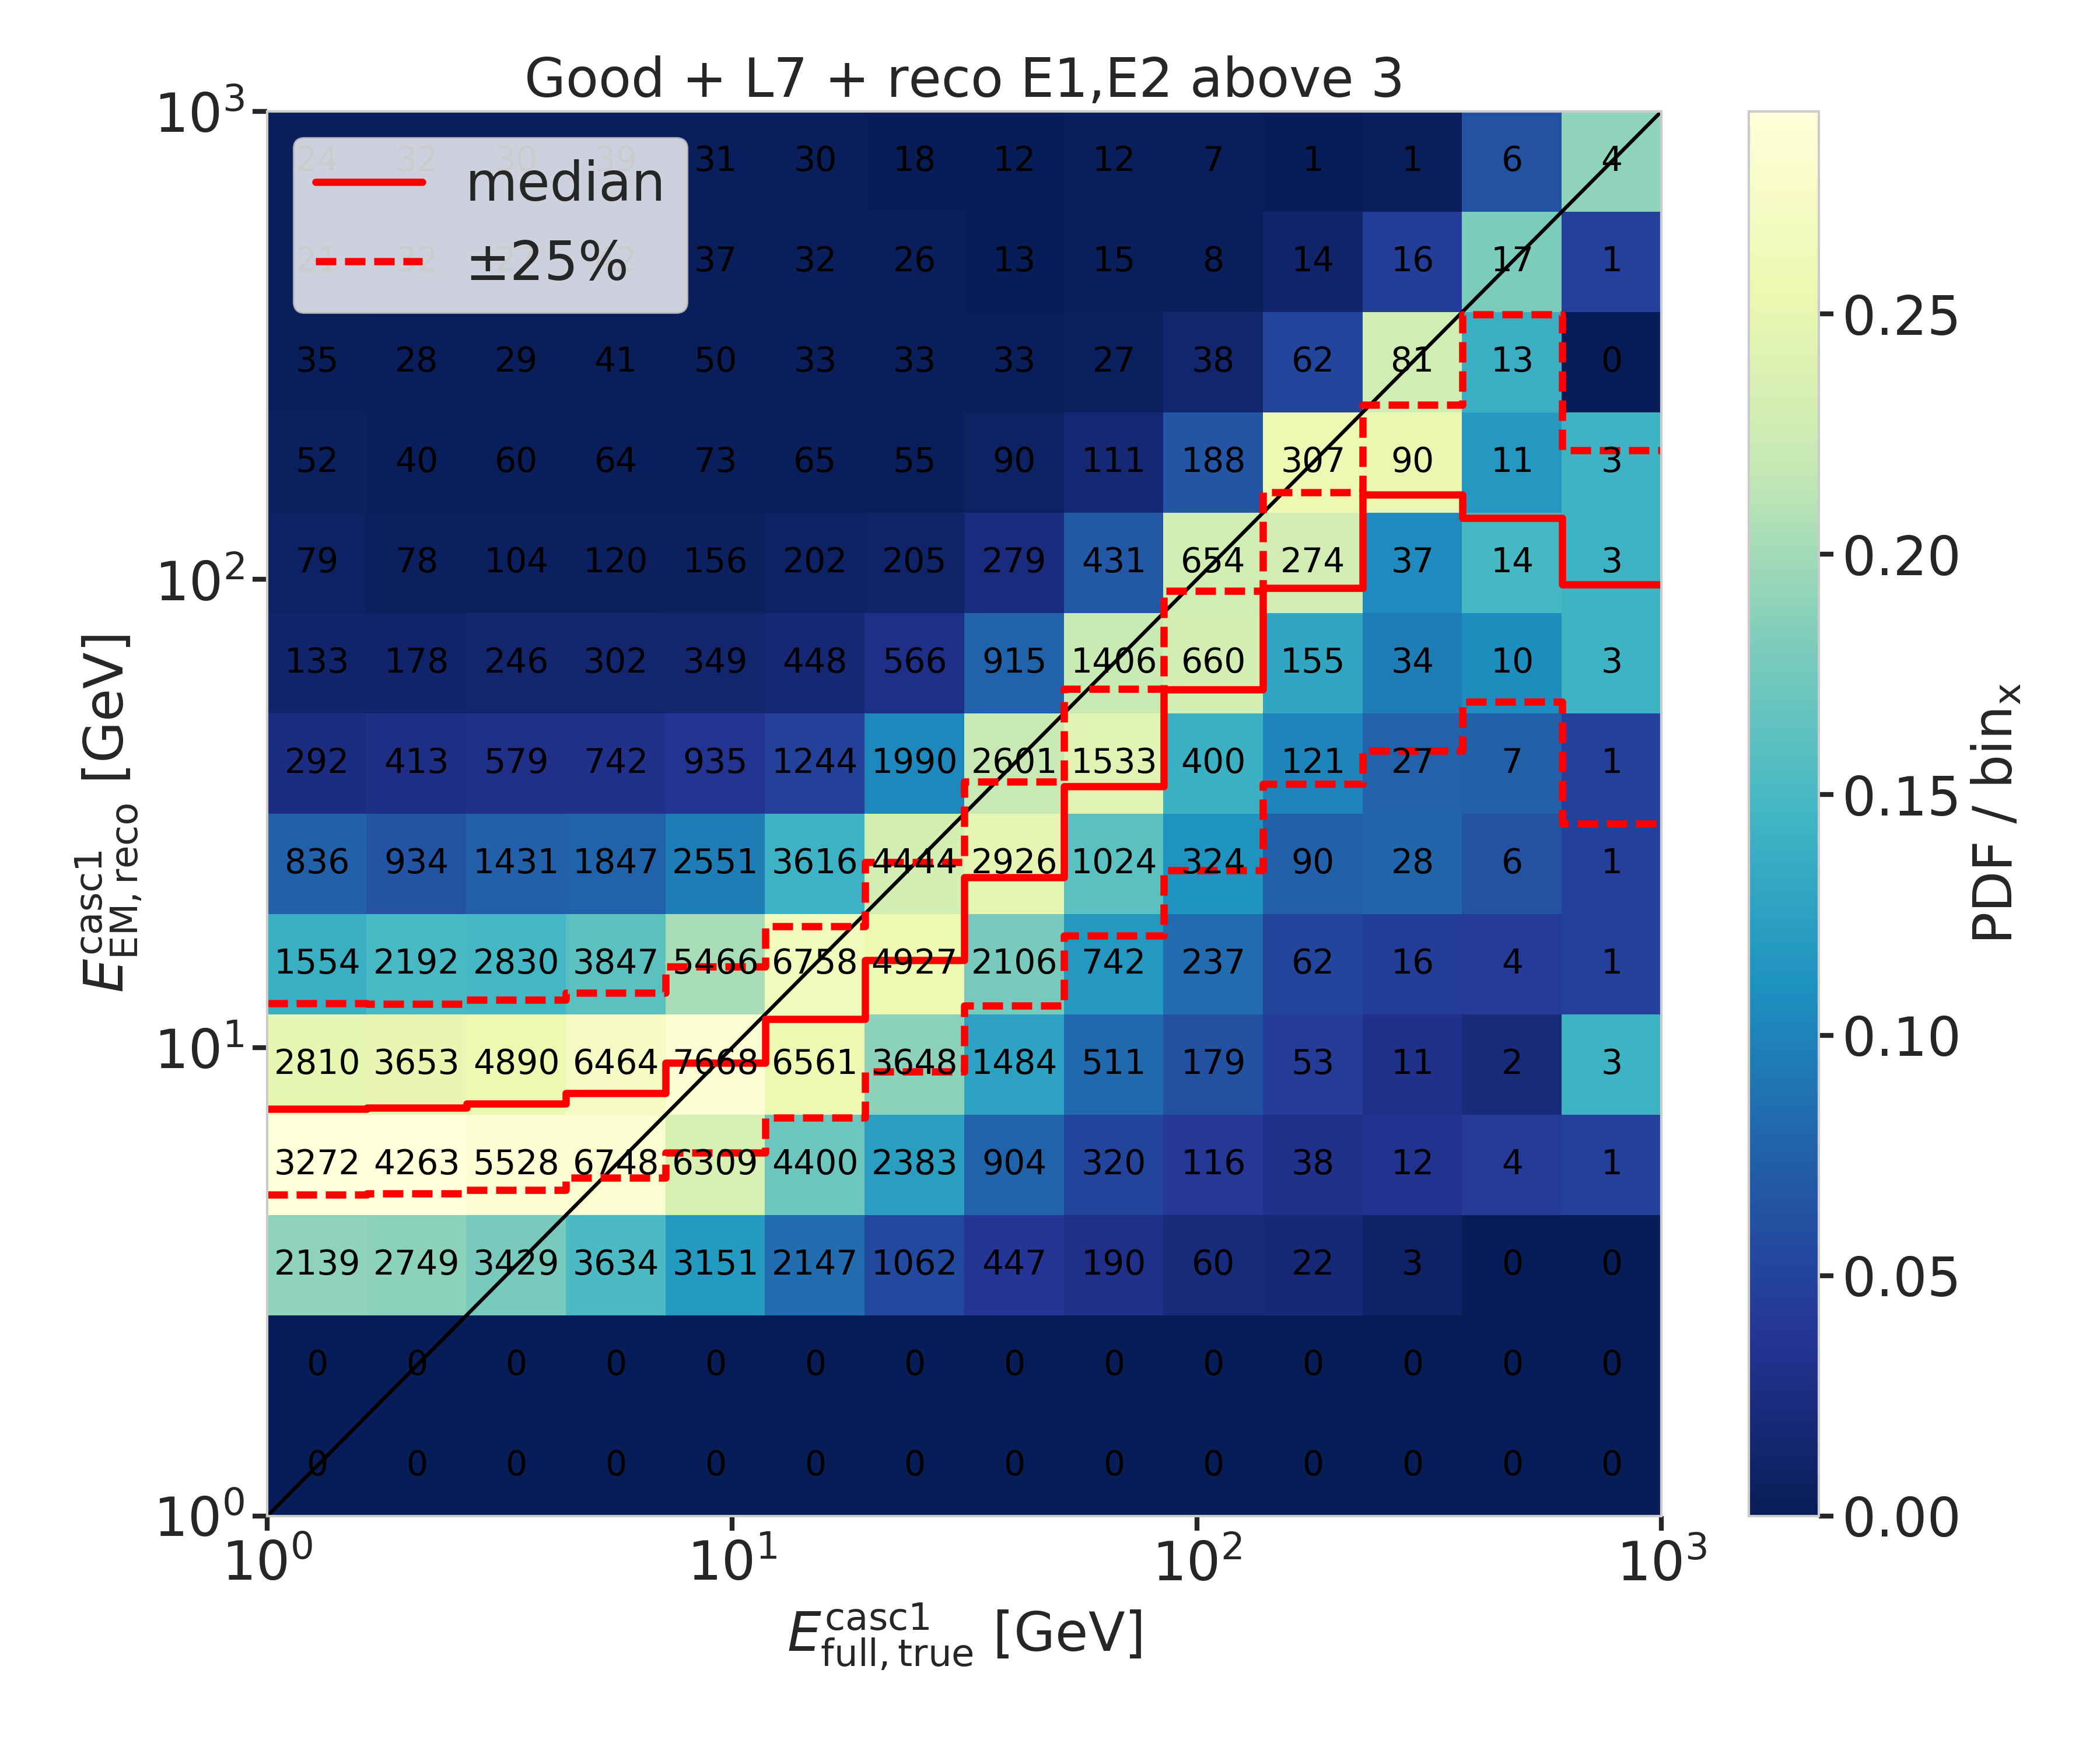
\includegraphics[width=0.49\linewidth]{figures/results/190607/resolutions/190607_millipede_level_no_NaNs_NEW_flipped_casc1_reco_energy_vs_casc1_true_energy_reco_above3_step_contours.png}
    \caption[Preliminary 2-d reconstructed versus true cascade energy resolutions]{Reconstructed (EM) energy versus true energy (full) energy for the first cascade (left) and second cascade (right). The color scale is according to the PDF in each vertical true energy slice, with the solid and dashed lines showing the median$\pm$\SI{25}{\percent} quantiles. The bin entries are shown as numbers.}
    \labfig{selected_routine_2d_energy_results}
\end{figure*}

The histogram for the first cascade energy is shown on the left and above an energy of $\sim$\SI{10}{\gev} the reconstruction performs well, with the median being parallel to the diagonal and the spread in the $\pm$\SI{25}{\percent} quantile being small. Below this energy the reconstruction is over-estimating the true energy, which is a known effect in IceCube, where the reconstruction is biased towards higher energies around the energy detection threshold, because events that enter the sample are events with an over fluctuation in their light deposition, which makes them pass into the selection and being reconstructible in the first place.

For the second cascade the overall behavior is similar, only that the energy where the reconstruction starts to perform good is higher around $\sim$\SI{20}{\gev}. The spread around the median is also larger and starts to expand a lot above \SI{200}{\gev}, where the statistics are lower as can be seen from the bin counts. It is also very apparent that the majority of energies of the second cascade are at lower true energy values between \SIrange[range-phrase=~and~]{1}{20}{\gev}.

For both cascade resolutions the effect of the reconstruction being biased towards lower values, due to the comparison of the full true energy to the reconstructed EM energy can be seen.


\subsubsection{Length Resolutions}

The decay length resolution is also investigated by looking at a similar style of 2-d histograms than for the energies, where the reconstructed decay length is plotted versus the true decay length. The left part of \reffig{selected_routine_2d_length_results} shows the distributions after the same selection criteria from \refsec{190607_energy_resolutions} are applied. It can be observed that for short true lengths the reconstruction is over-estimating the length, while for long true lengths the reconstruction is strongly under-estimating the length. There is a region between true lengths of \SIrange[range-phrase=~and~]{20}{80}{\meter} where the median reconstruction is almost unbiased, but the \SI{50}{\percent} interquartile range is large and increasing from $\sim$\SI{50}{\meter} to $\sim$\SI{70}{\meter} with true decay lengths.

\begin{figure*}[h]
    \centering
    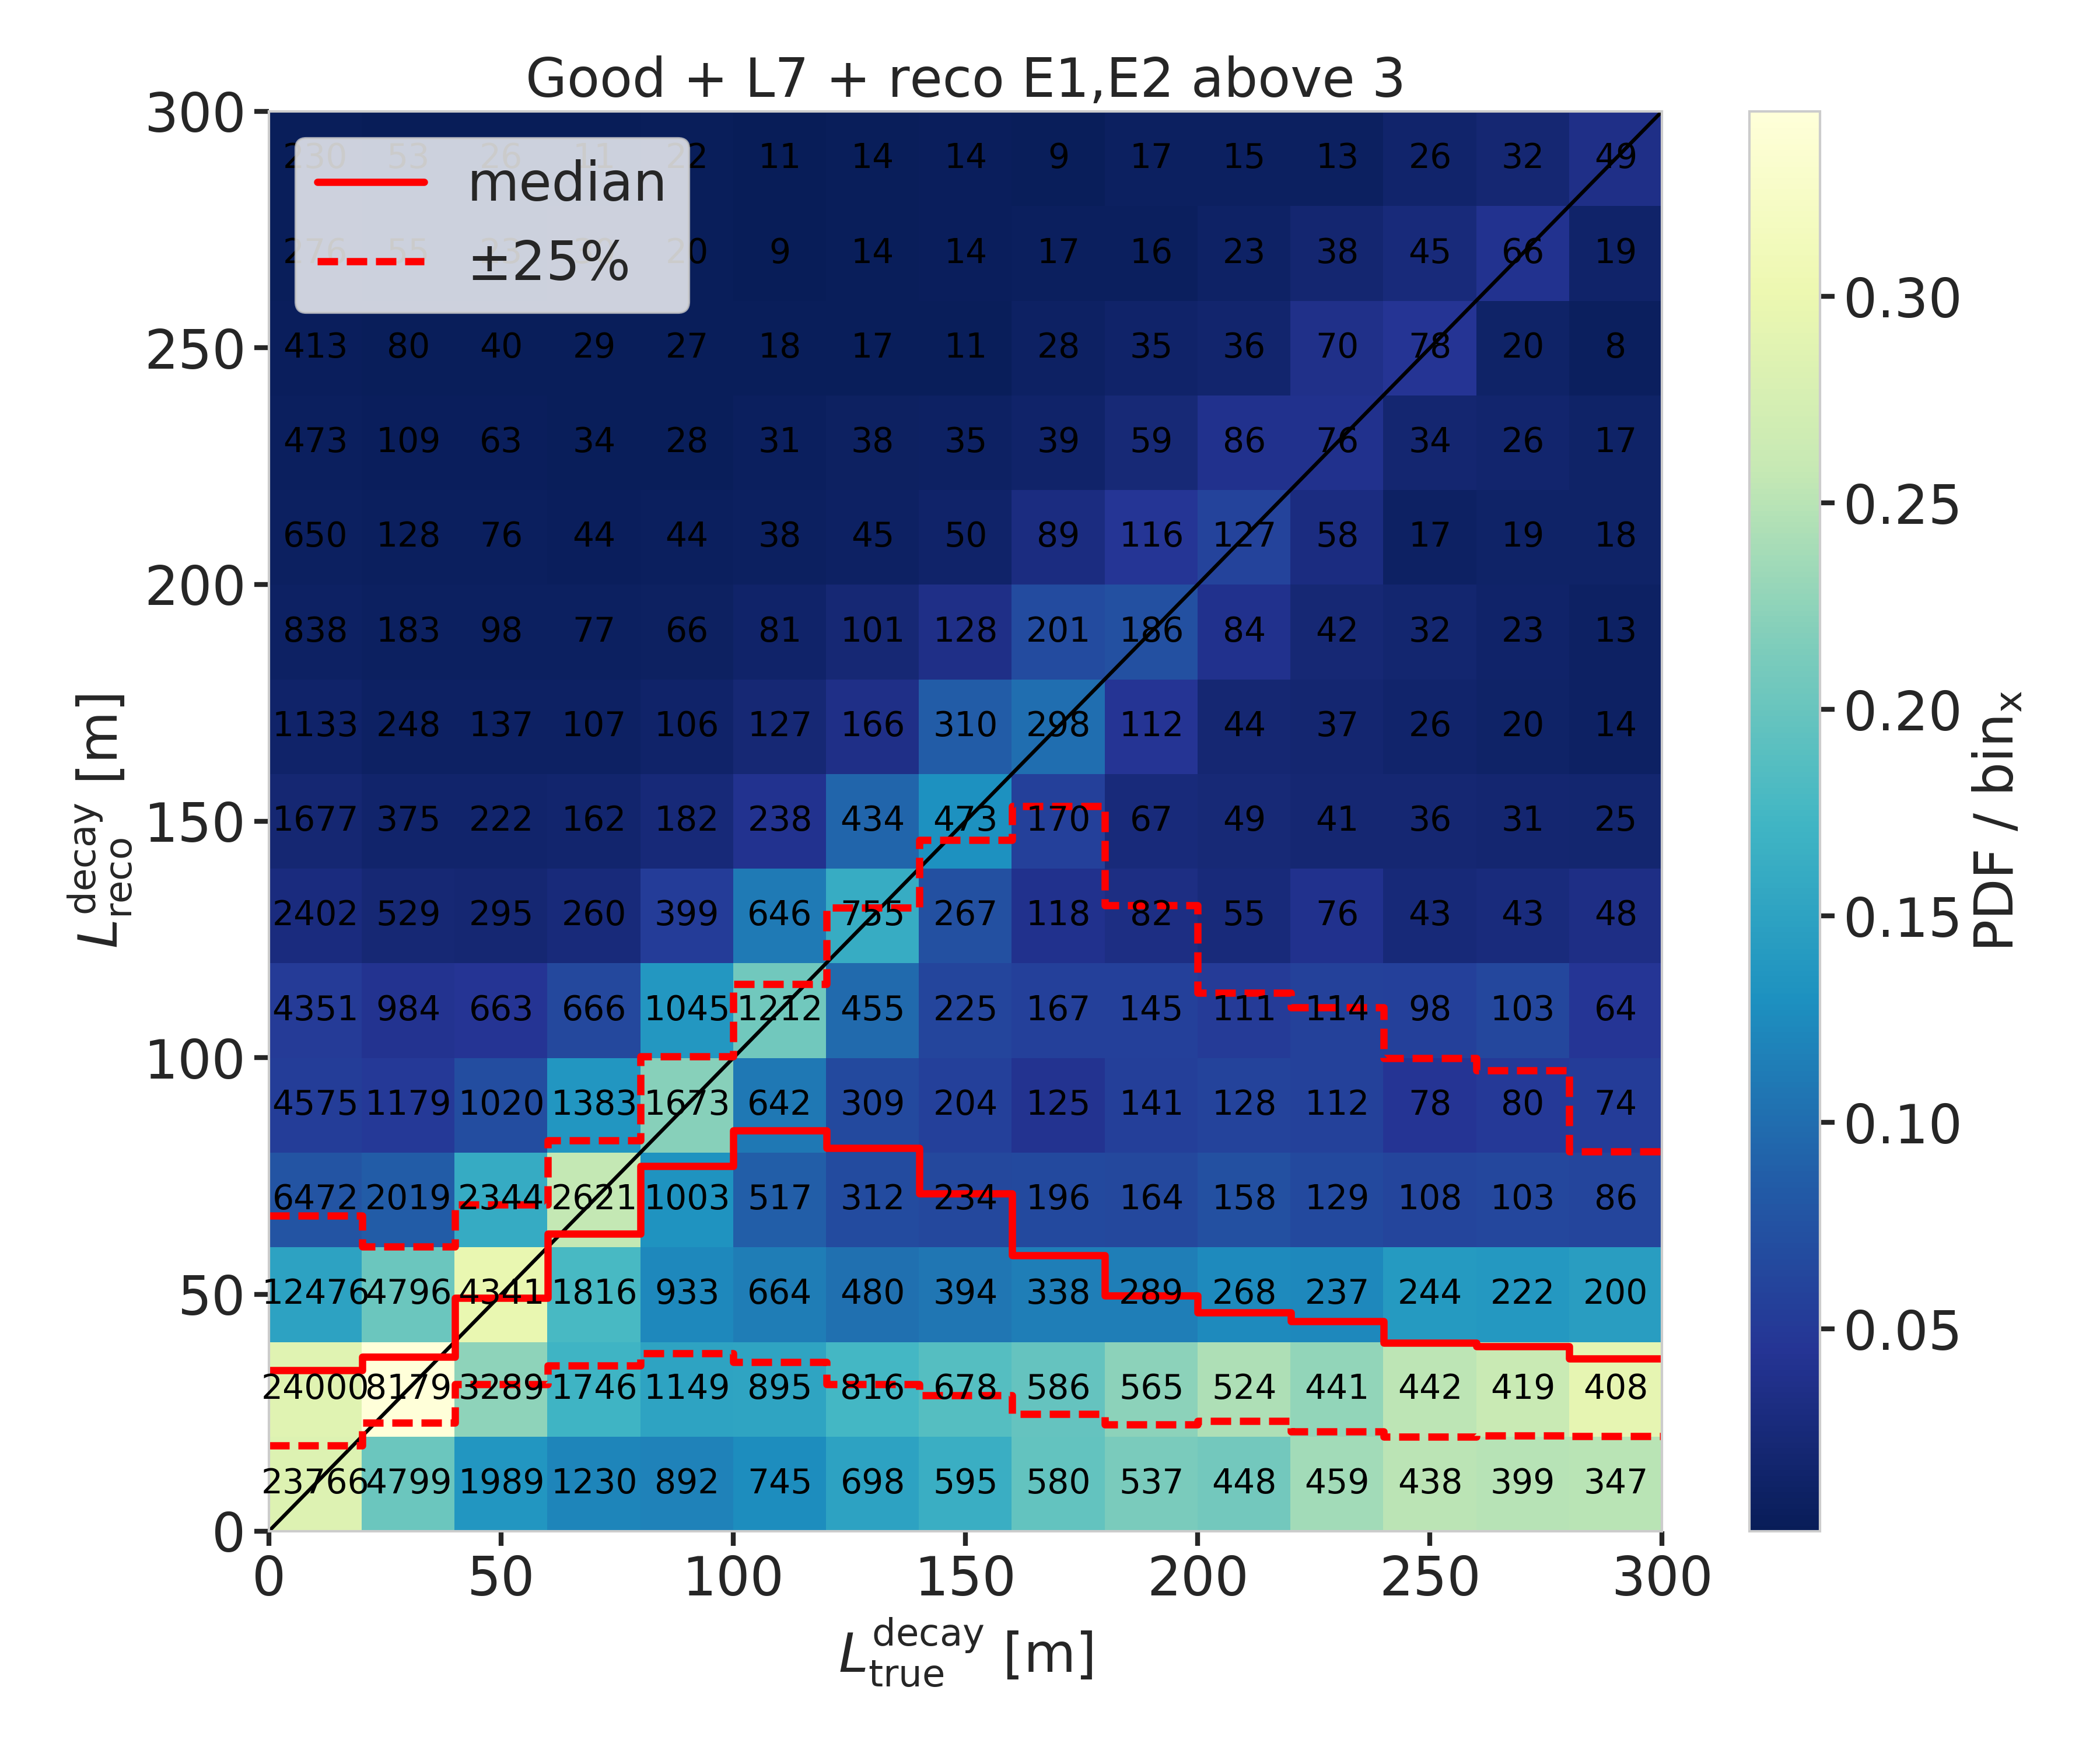
\includegraphics[width=0.49\linewidth]{figures/results/190607/resolutions/190607_millipede_level_no_NaNs_NEW_flipped_reco_decayL_vs_true_decayL_reco_above3_step_contours.png}
    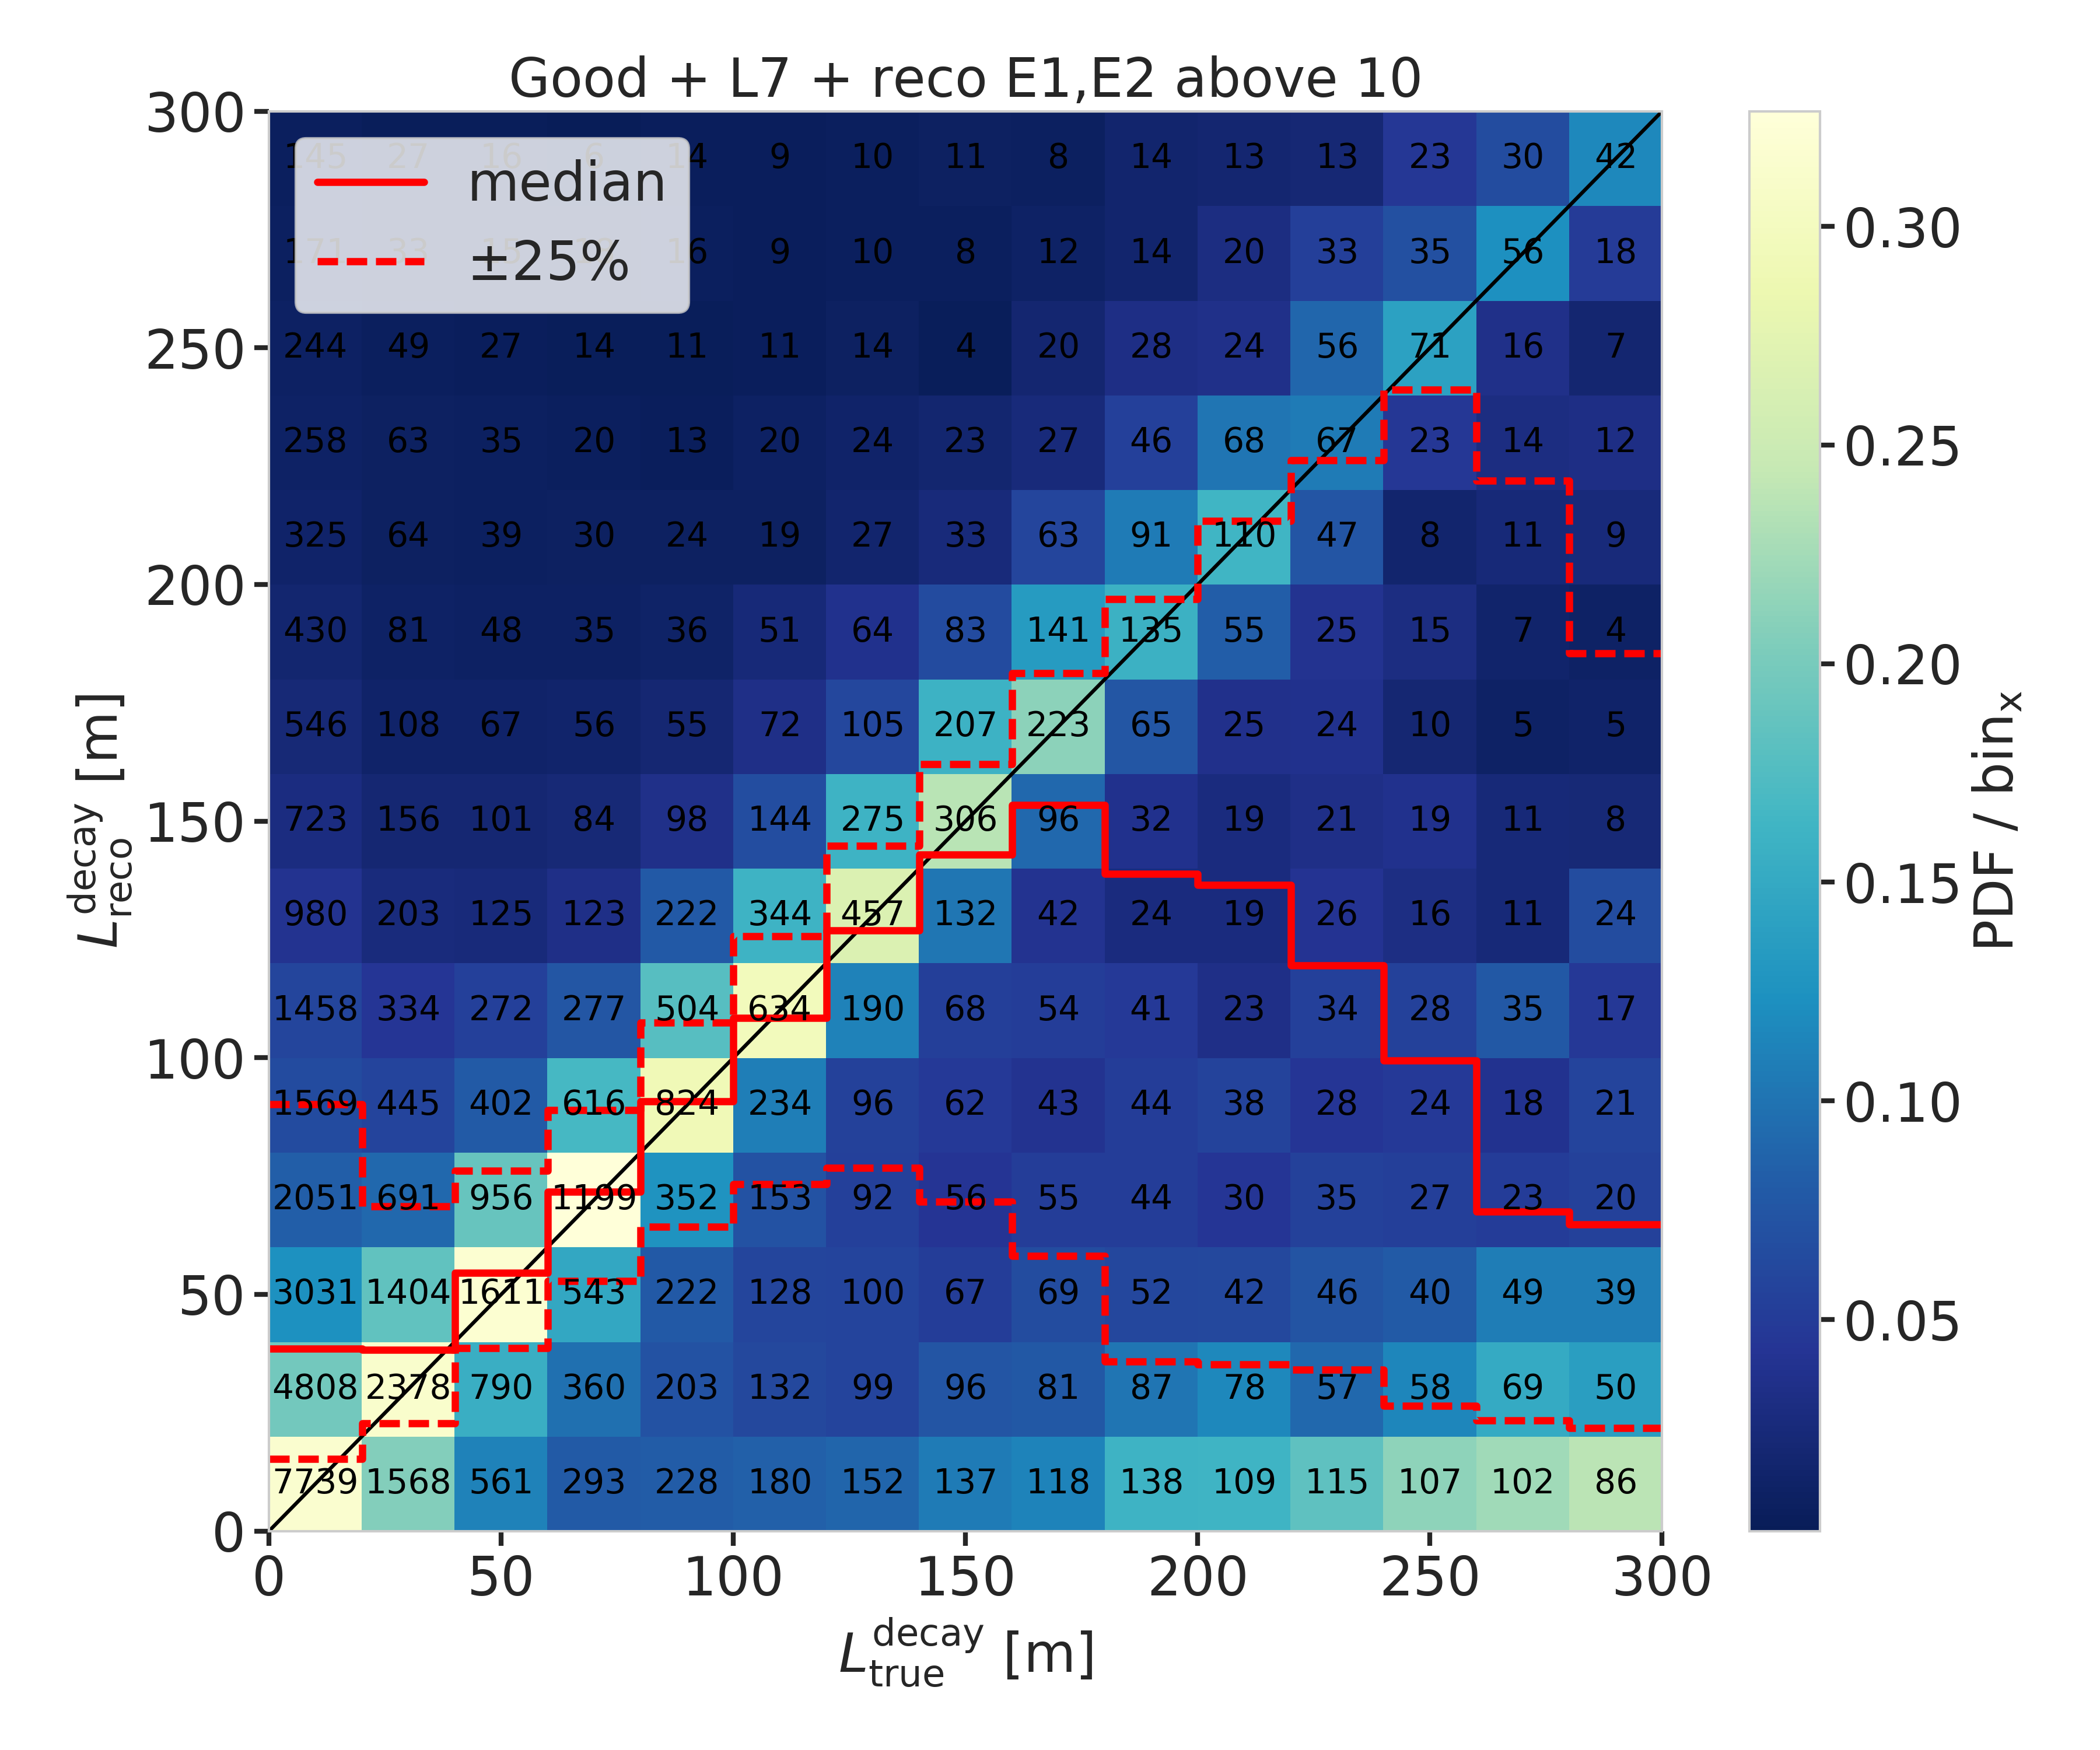
\includegraphics[width=0.49\linewidth]{figures/results/190607/resolutions/190607_millipede_level_no_NaNs_NEW_flipped_reco_decayL_vs_true_decayL_reco_above10_step_contours.png}
    \caption[Preliminary 2-d reconstructed versus true decay length resolutions]{Reconstructed decay length versus true decay length for $\sim$\SI{3}{\gev} (left) and $\sim$\SI{10}{\gev} (right) minimum reconstructed cascade energies. The color scale is according to the PDF in each vertical true length slice, with the solid and dashed lines showing the median$\pm$\SI{25}{\percent} quantiles. The bin entries are shown as numbers.}
    \labfig{selected_routine_2d_length_results}
\end{figure*}

The over-estimation at small true lengths can be explained for multiple reasons, one being that the shortest DOM spacing is $\sim$\SI{7}{\meter}, vertically for DeepCore strings, but mostly larger than that, so resolving lengths below this is very complicated, and the reconstruction tends to be biased towards estimating the length around where the light was observed. Another reason is a similar argument to why the energies are over-estimated at small true values, namely that events that passed the selection and were reconstructed in those cases, probably have an over fluctuation in light deposition, extending further out from the vertices, so the reconstructed length is larger. Additionally, approaching a length of 0.0, the reconstructed length will of course always be a one-sided distribution, because the lengths have to be positive.

The under-estimation at large true lengths is more puzzling, and it seems like the distribution becomes bimodal in the reconstructed lengths, with on population around the diagonal, meaning that they are properly reconstructed, and one population at very short reconstructed lengths, which are badly reconstructed. Above \SI{150}{\meter} the badly reconstructed population starts to dominate, and the median resolution drops off strongly. The assumption is that for these events, only one cascade was observed with enough light to be reconstructed, and the reconstruction describes the one observed cascade in two parts, separated by a short distance, driven by similar factors as mentioned before. A check to confirm whether this is the case was to increase the minimum cascade energies to \SI{10}{\gev}, which is shown in the right part of \reffig{selected_routine_2d_length_results}. It can be seen that the median resolution is already much better, aligning with the expectation between \SIrange[range-phrase=~and~]{40}{160}{\meter}. Judging from the median resolution and the $+$\SI{25}{\percent} quantile in this range, there is very few events with an over-expectation in the energy, since both of them are alidgning with the diagonal. The spread towards lower reconstructed lengths, on the other hand, is still very large and above \SI{200}{\meter} the badly reconstructed population starts to dominate again.


% \begin{figure*}[h]
% 	\centering
%     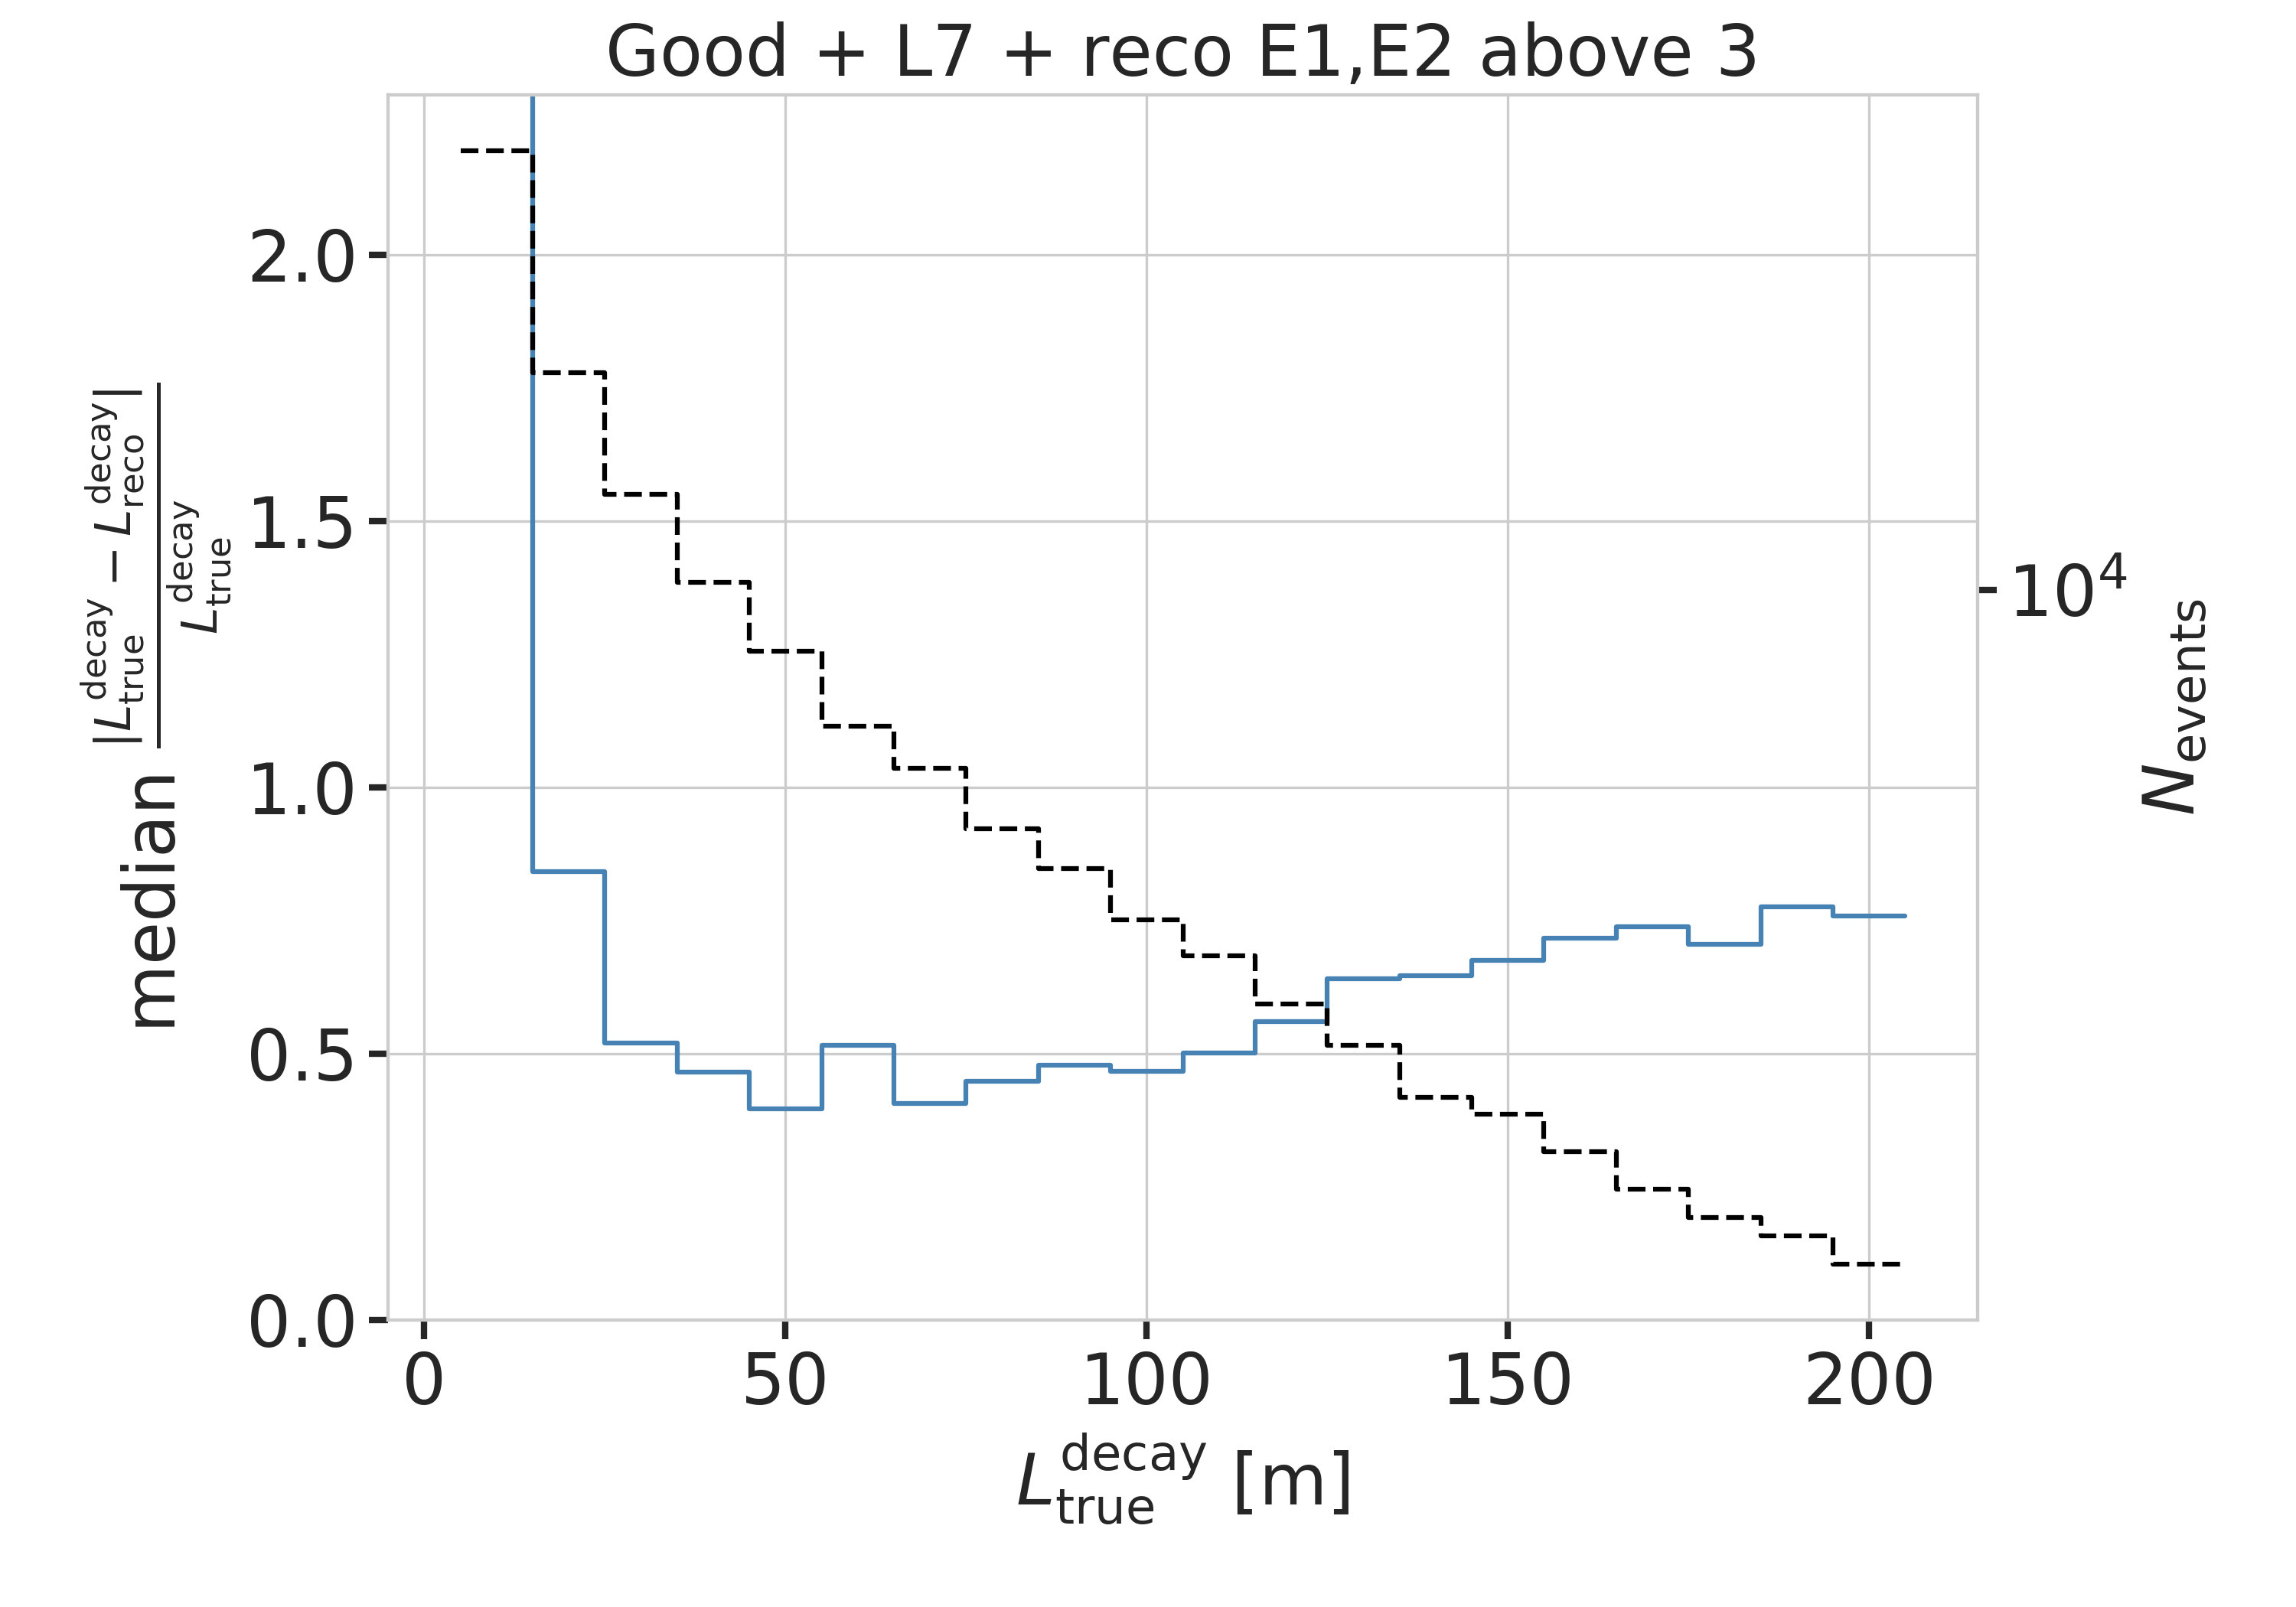
\includegraphics[width=0.49\linewidth]{figures/results/190607/resolutions/median_decay_length_resolution_Good + L7 + reco E1,E2 above 3_n_events.png}
%     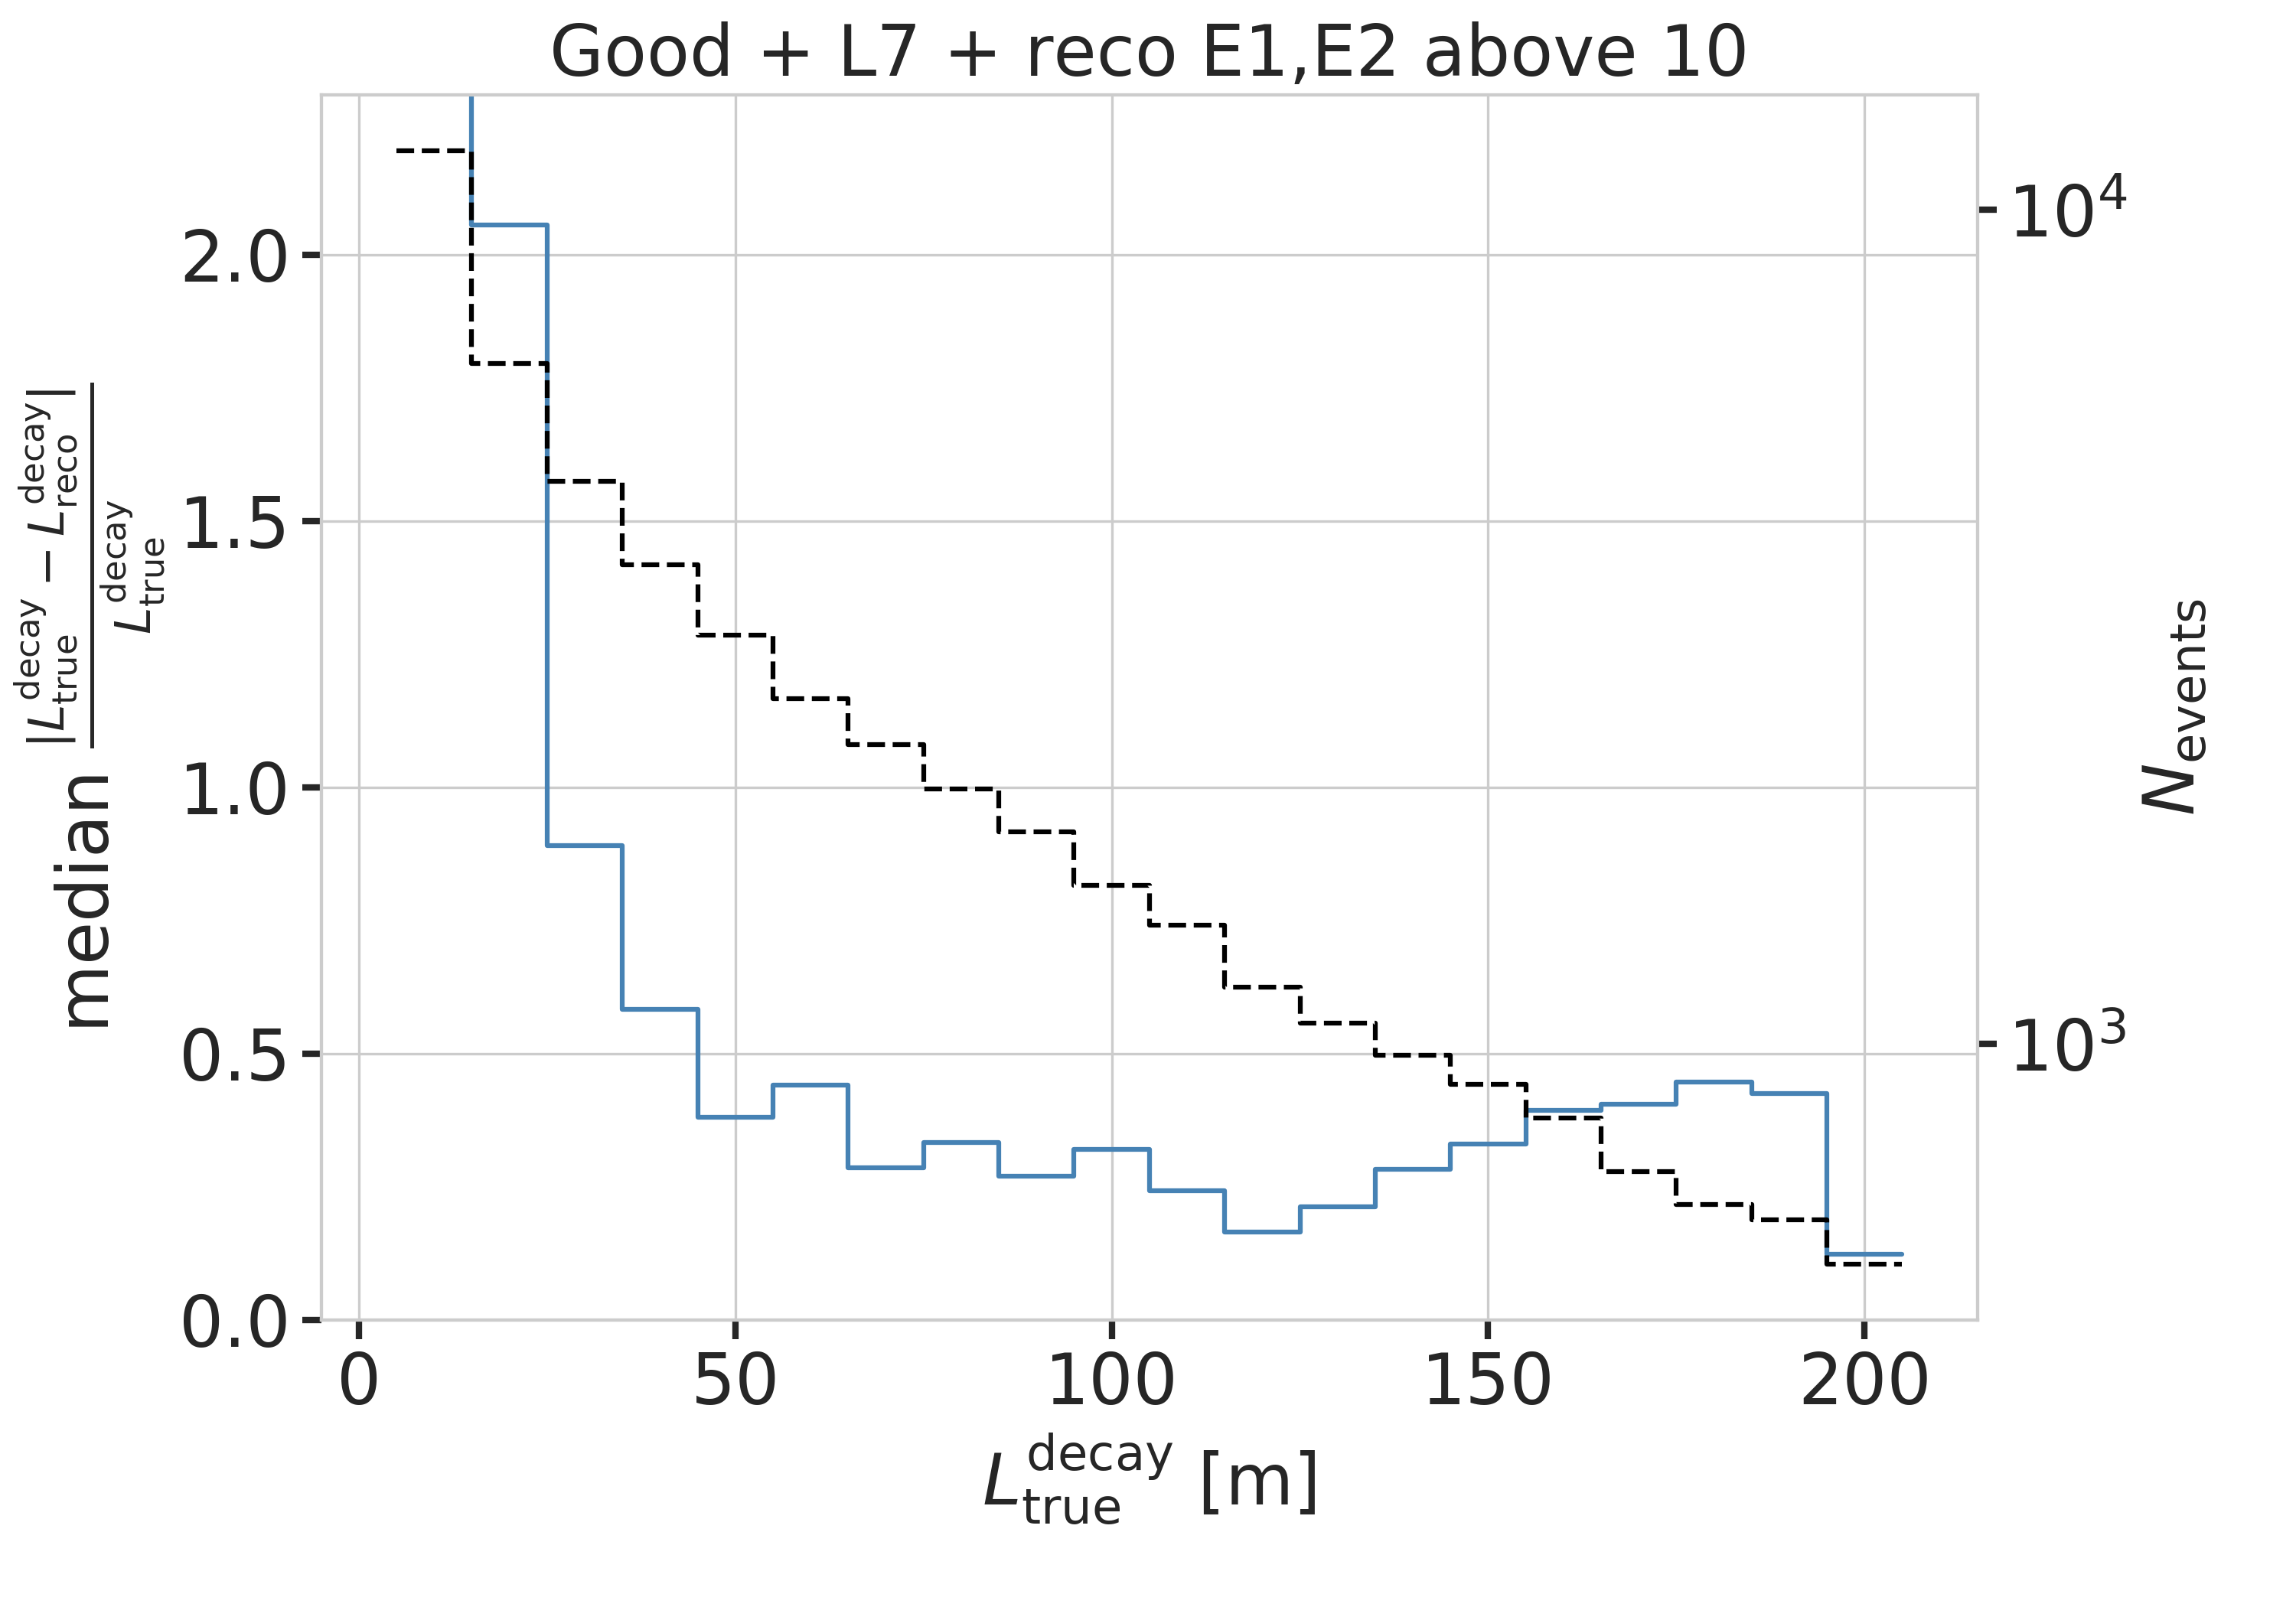
\includegraphics[width=0.49\linewidth]{figures/results/190607/resolutions/median_decay_length_resolution_Good + L7 + reco E1,E2 above 10_n_events.png}  
%     \caption[]{}
%     \labfig{selected_routine_1d_length_results}
% \end{figure*}
% \todo{fix caption of this figure (RED)}



\subsubsection{Badly Reconstructed Cascade Population}

\paragraph{Ideas to write about:}
\begin{itemize}
    \item Show/highlight 2d decay length resolution again, basically 2 populations at higher energies
    \item only looking at events with >10 GeV instead of >3 GeV already improves the resolution a lot (low energy and therefore low light is a problem)
    \item take a closer look at those populations to find out what's going on
    \item multiple things were checked (bad direction (possibly due to seed), cascade position in DC, energies)
    \item the direction is worse for the badly reconstructed population, which could be due to a bad seed direction
    \item the events are a little further out radially, where the string/DOM spacing is not so tight, which also leads to less light being observed
    \item the energy of the second cascade is much lower than the first
    \item conclusion: it's a combination of all of them, but the main problem is the low energy
    \item true energies vs true length shows that first cascade energies are much larger than second (pick benchmark lengths and state the values!)
\end{itemize}

\begin{figure*}[h]
    \centering
    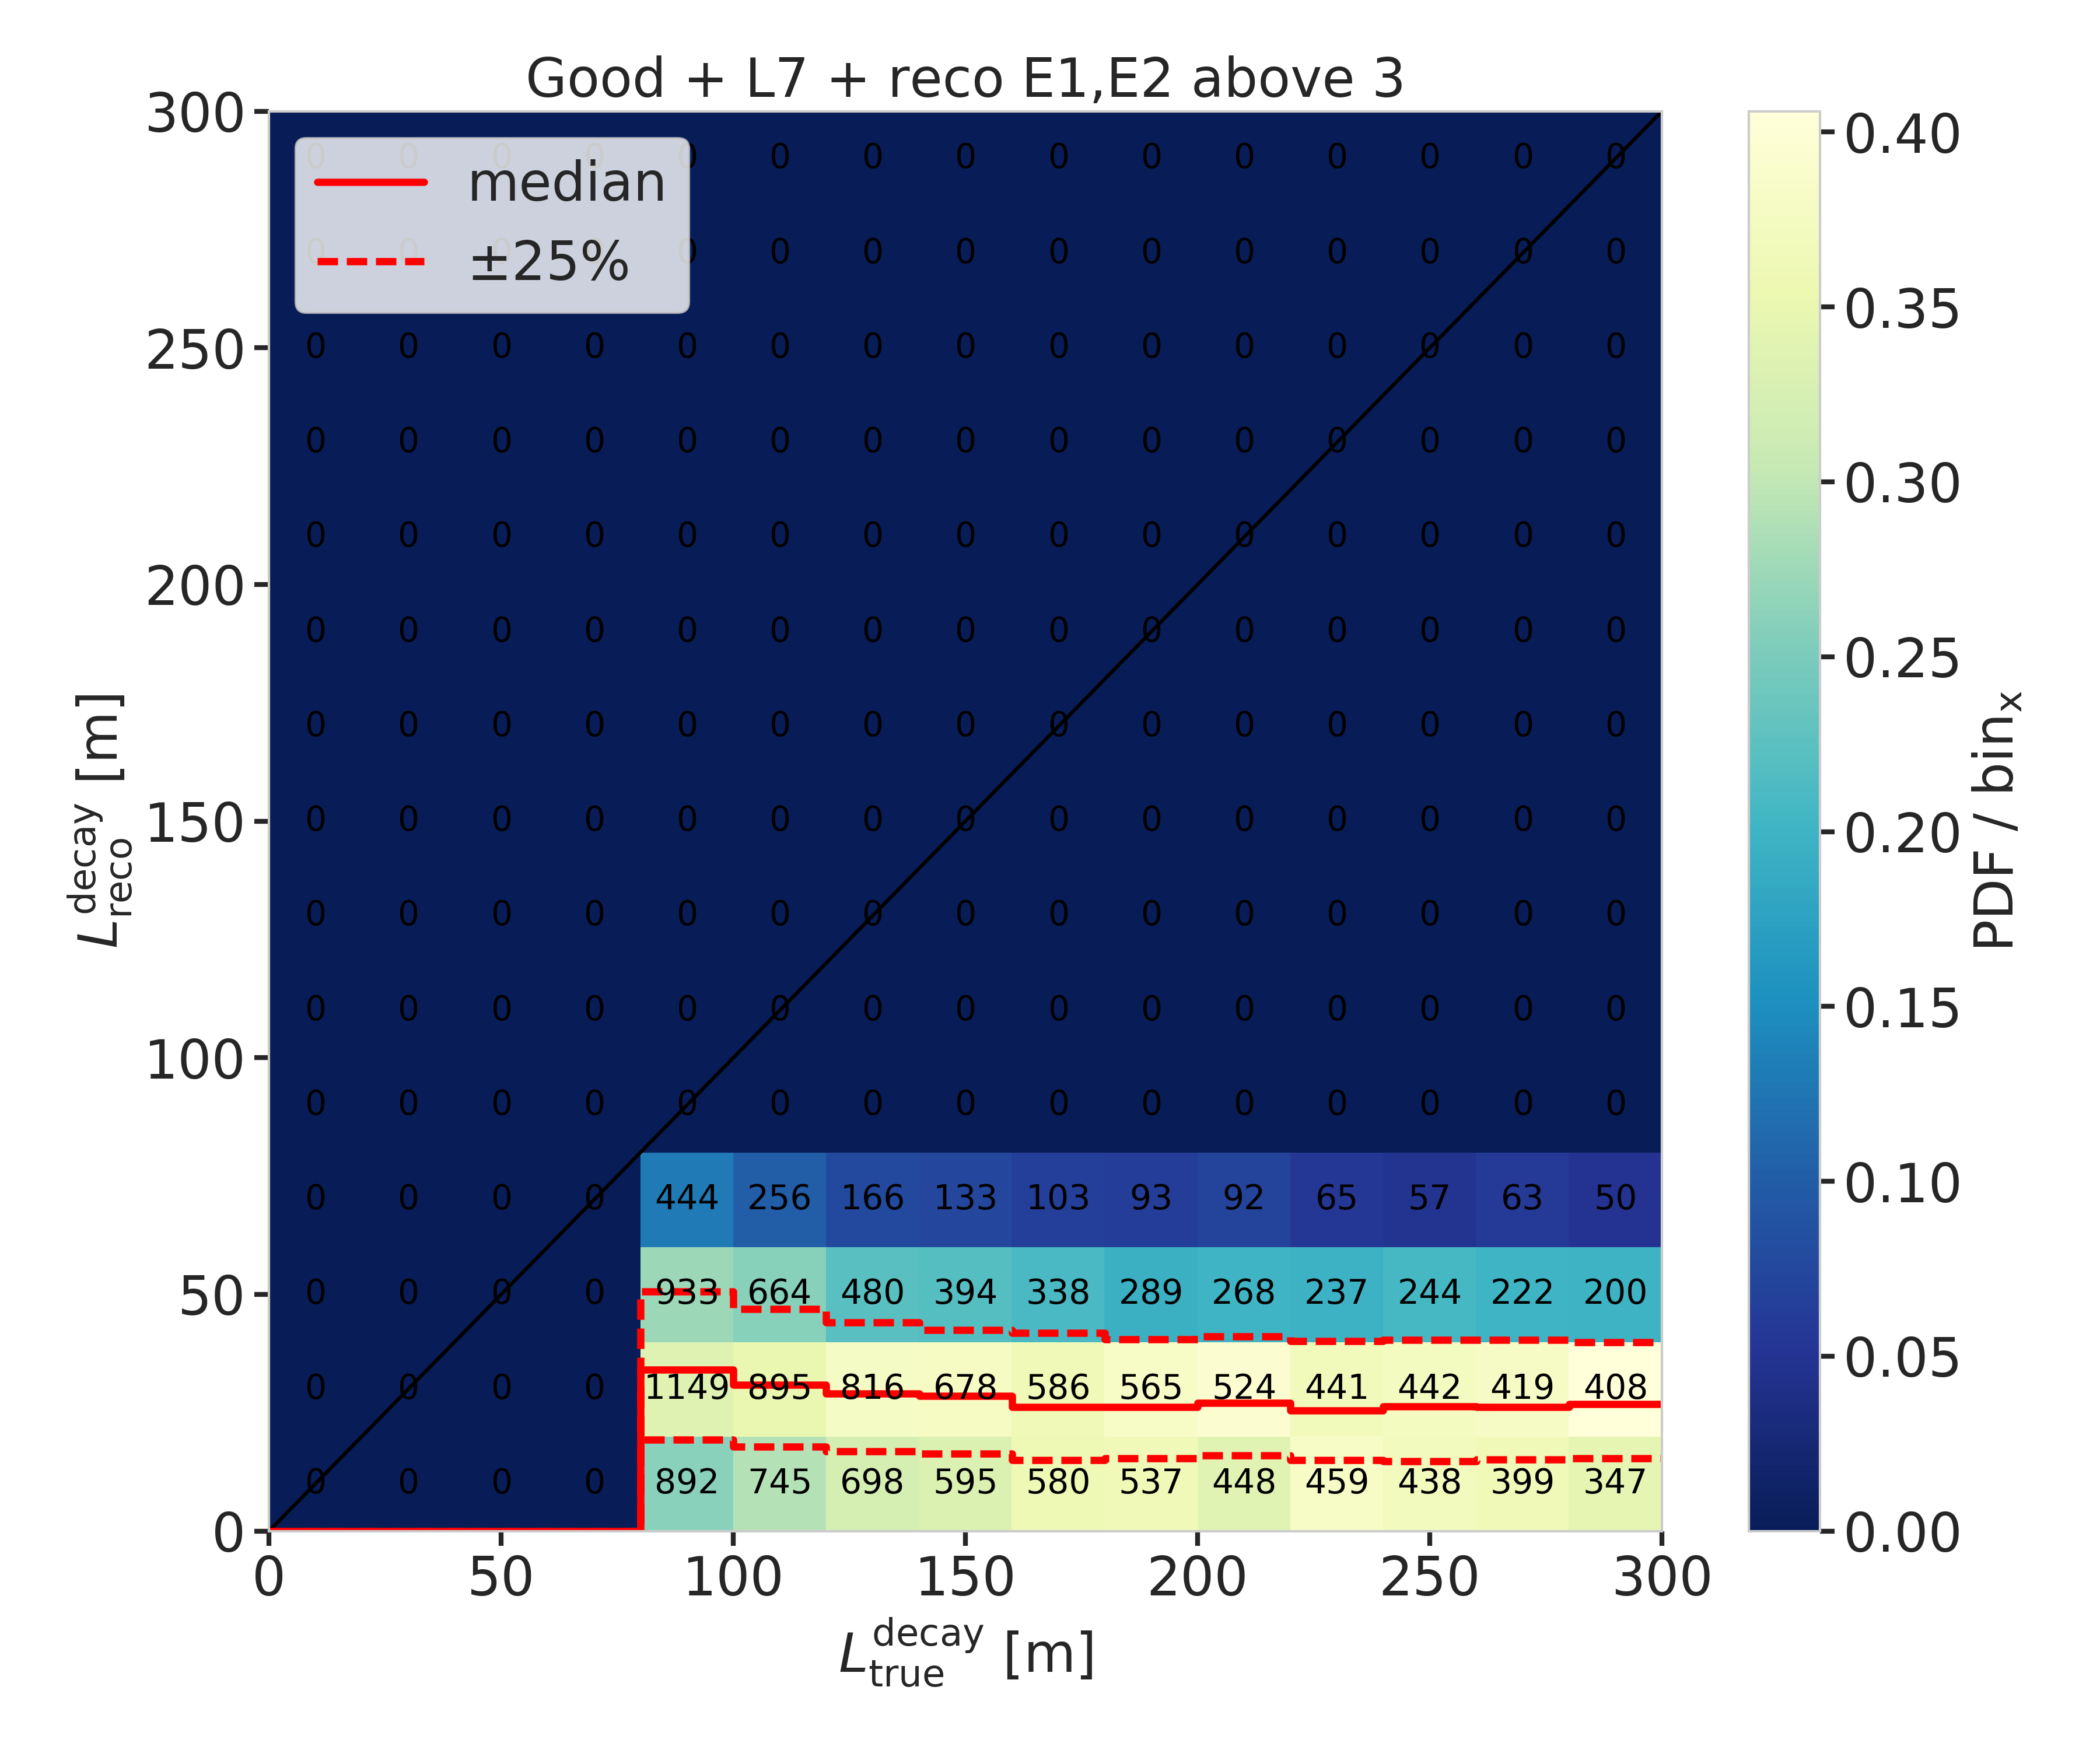
\includegraphics[width=0.49\linewidth]{figures/results/190607/second_population/190607_millipede_level_no_NaNs_NEW_flipped_reco_decayL_vs_true_decayL_reco_above3_population_in_step_contours.png}
    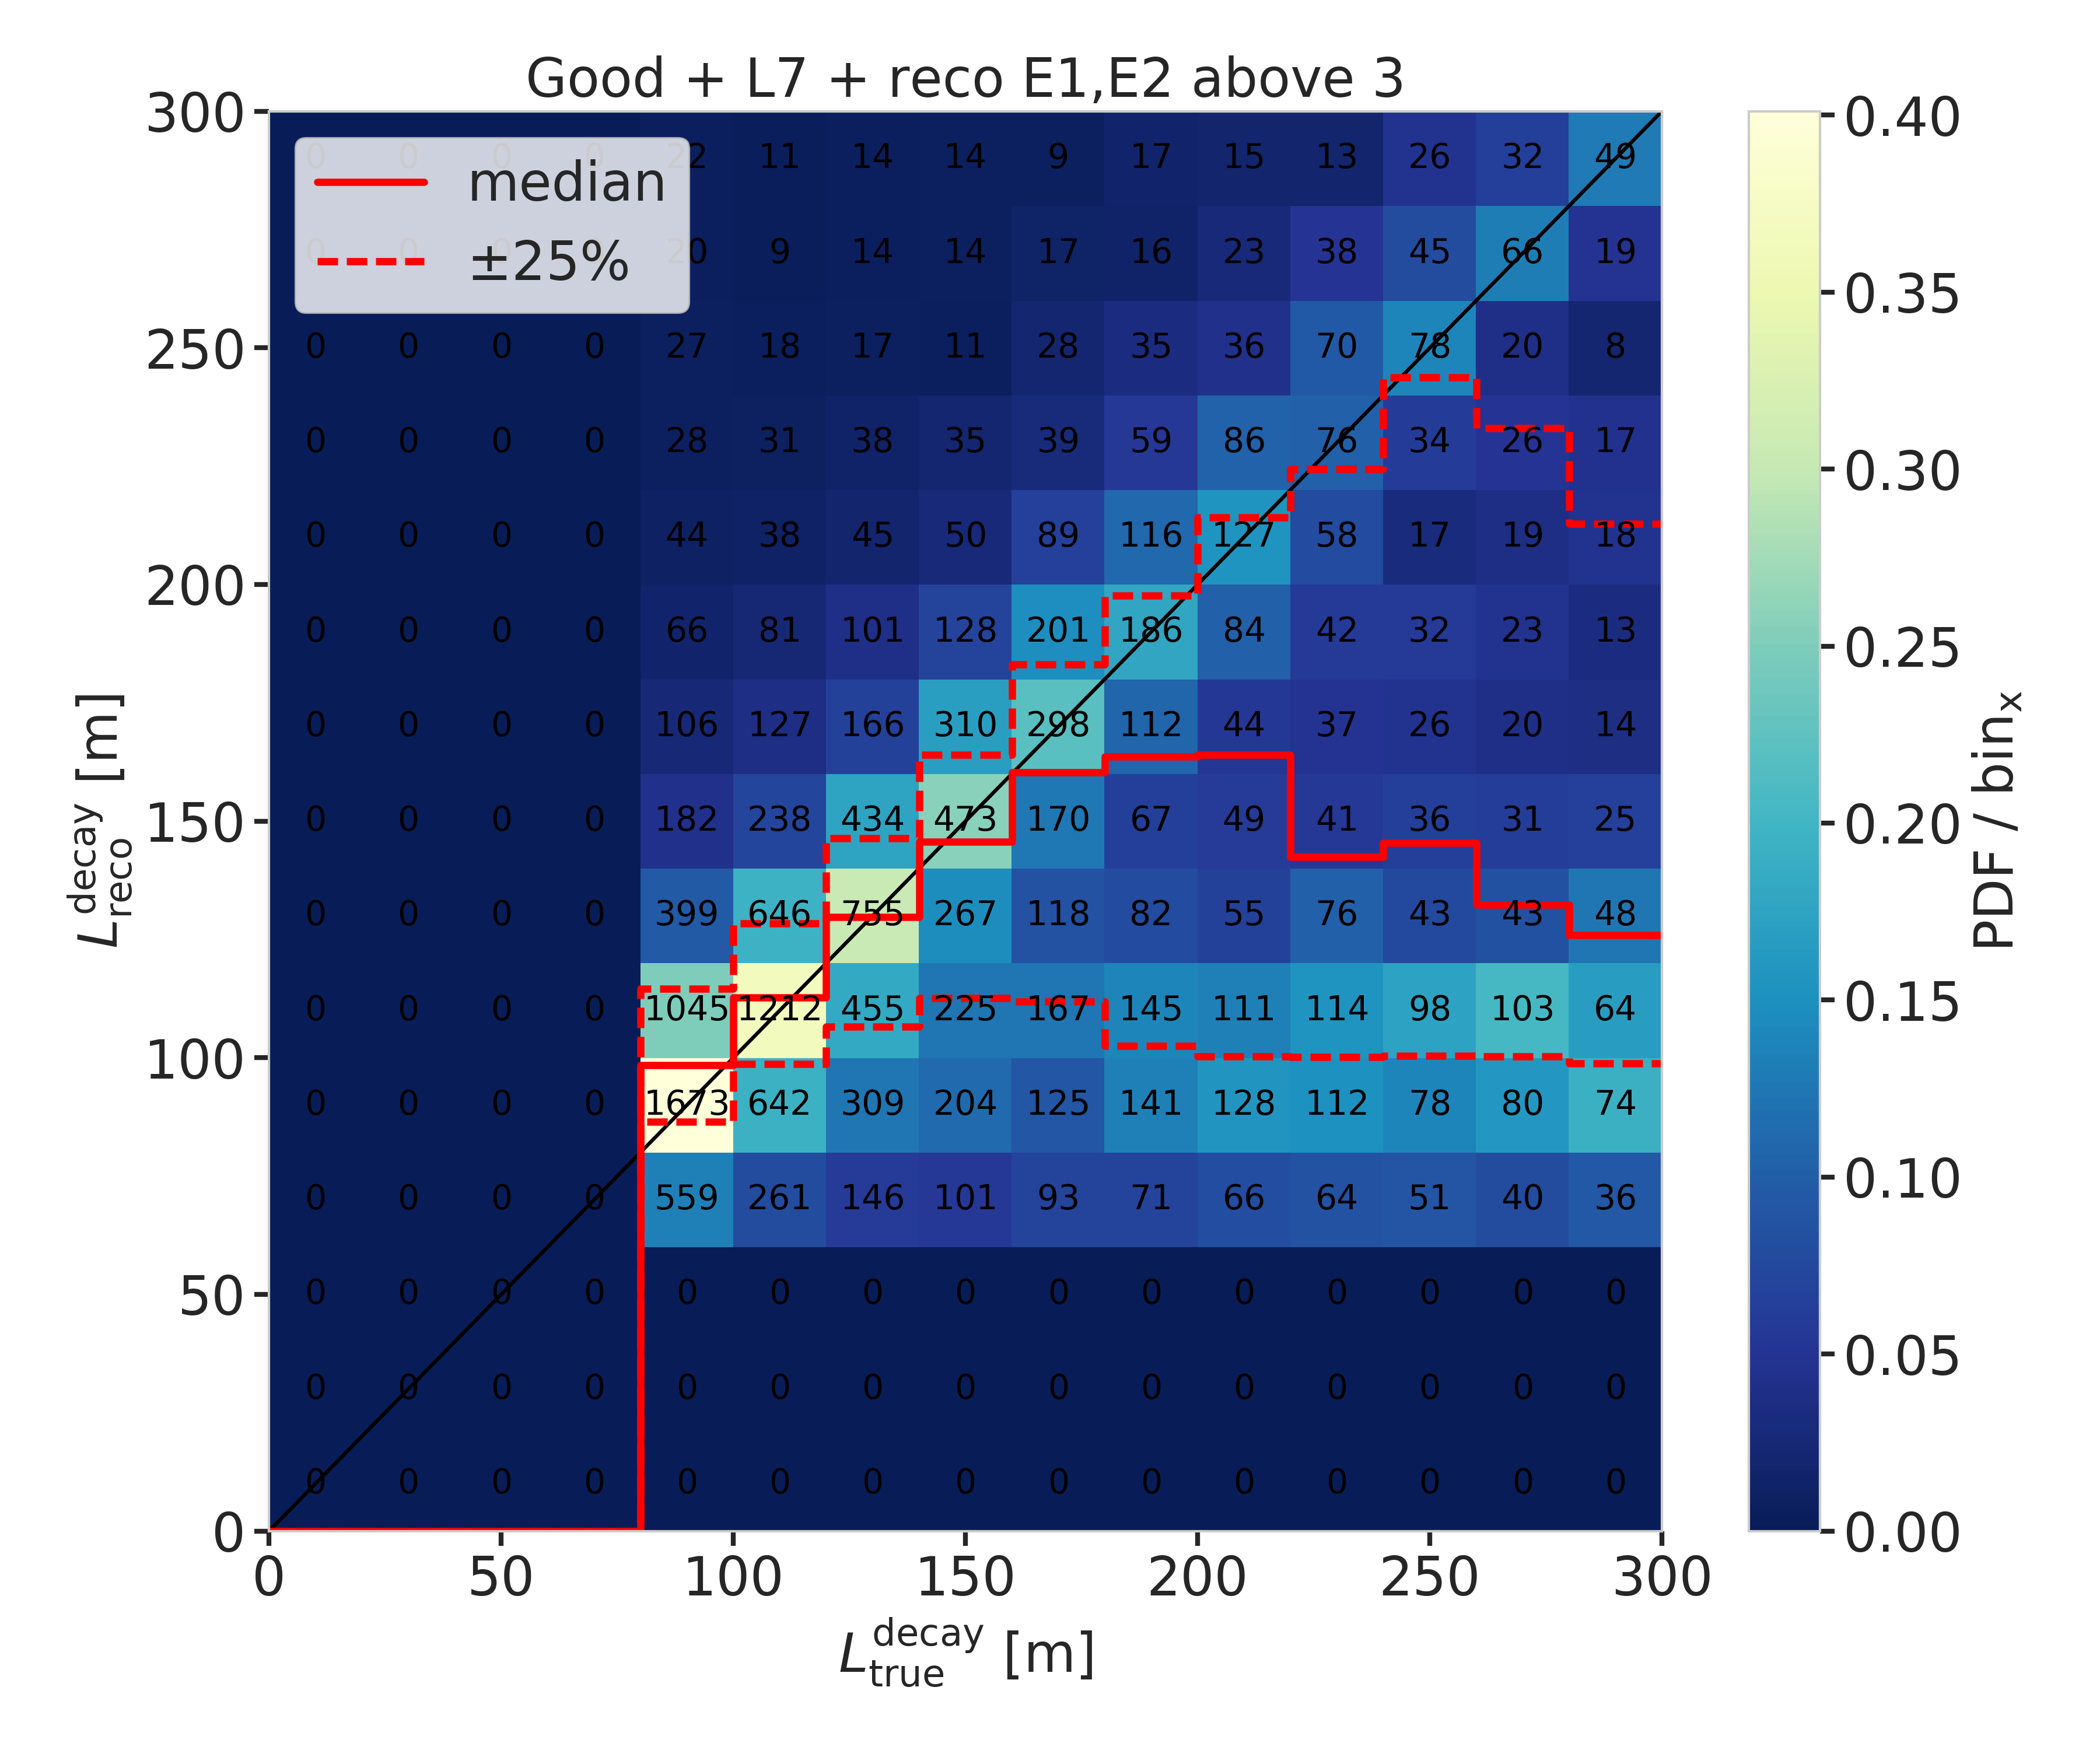
\includegraphics[width=0.49\linewidth]{figures/results/190607/second_population/190607_millipede_level_no_NaNs_NEW_flipped_reco_decayL_vs_true_decayL_reco_above3_population_out_step_contours.png}
    \caption[]{}
    \labfig{true_energies_vs_true_length}
\end{figure*}
\todo{make on figure, where the two selected regions are highlighted? (RED)}
\todo{fix caption (RED)}

\begin{figure*}[h]
    \centering
    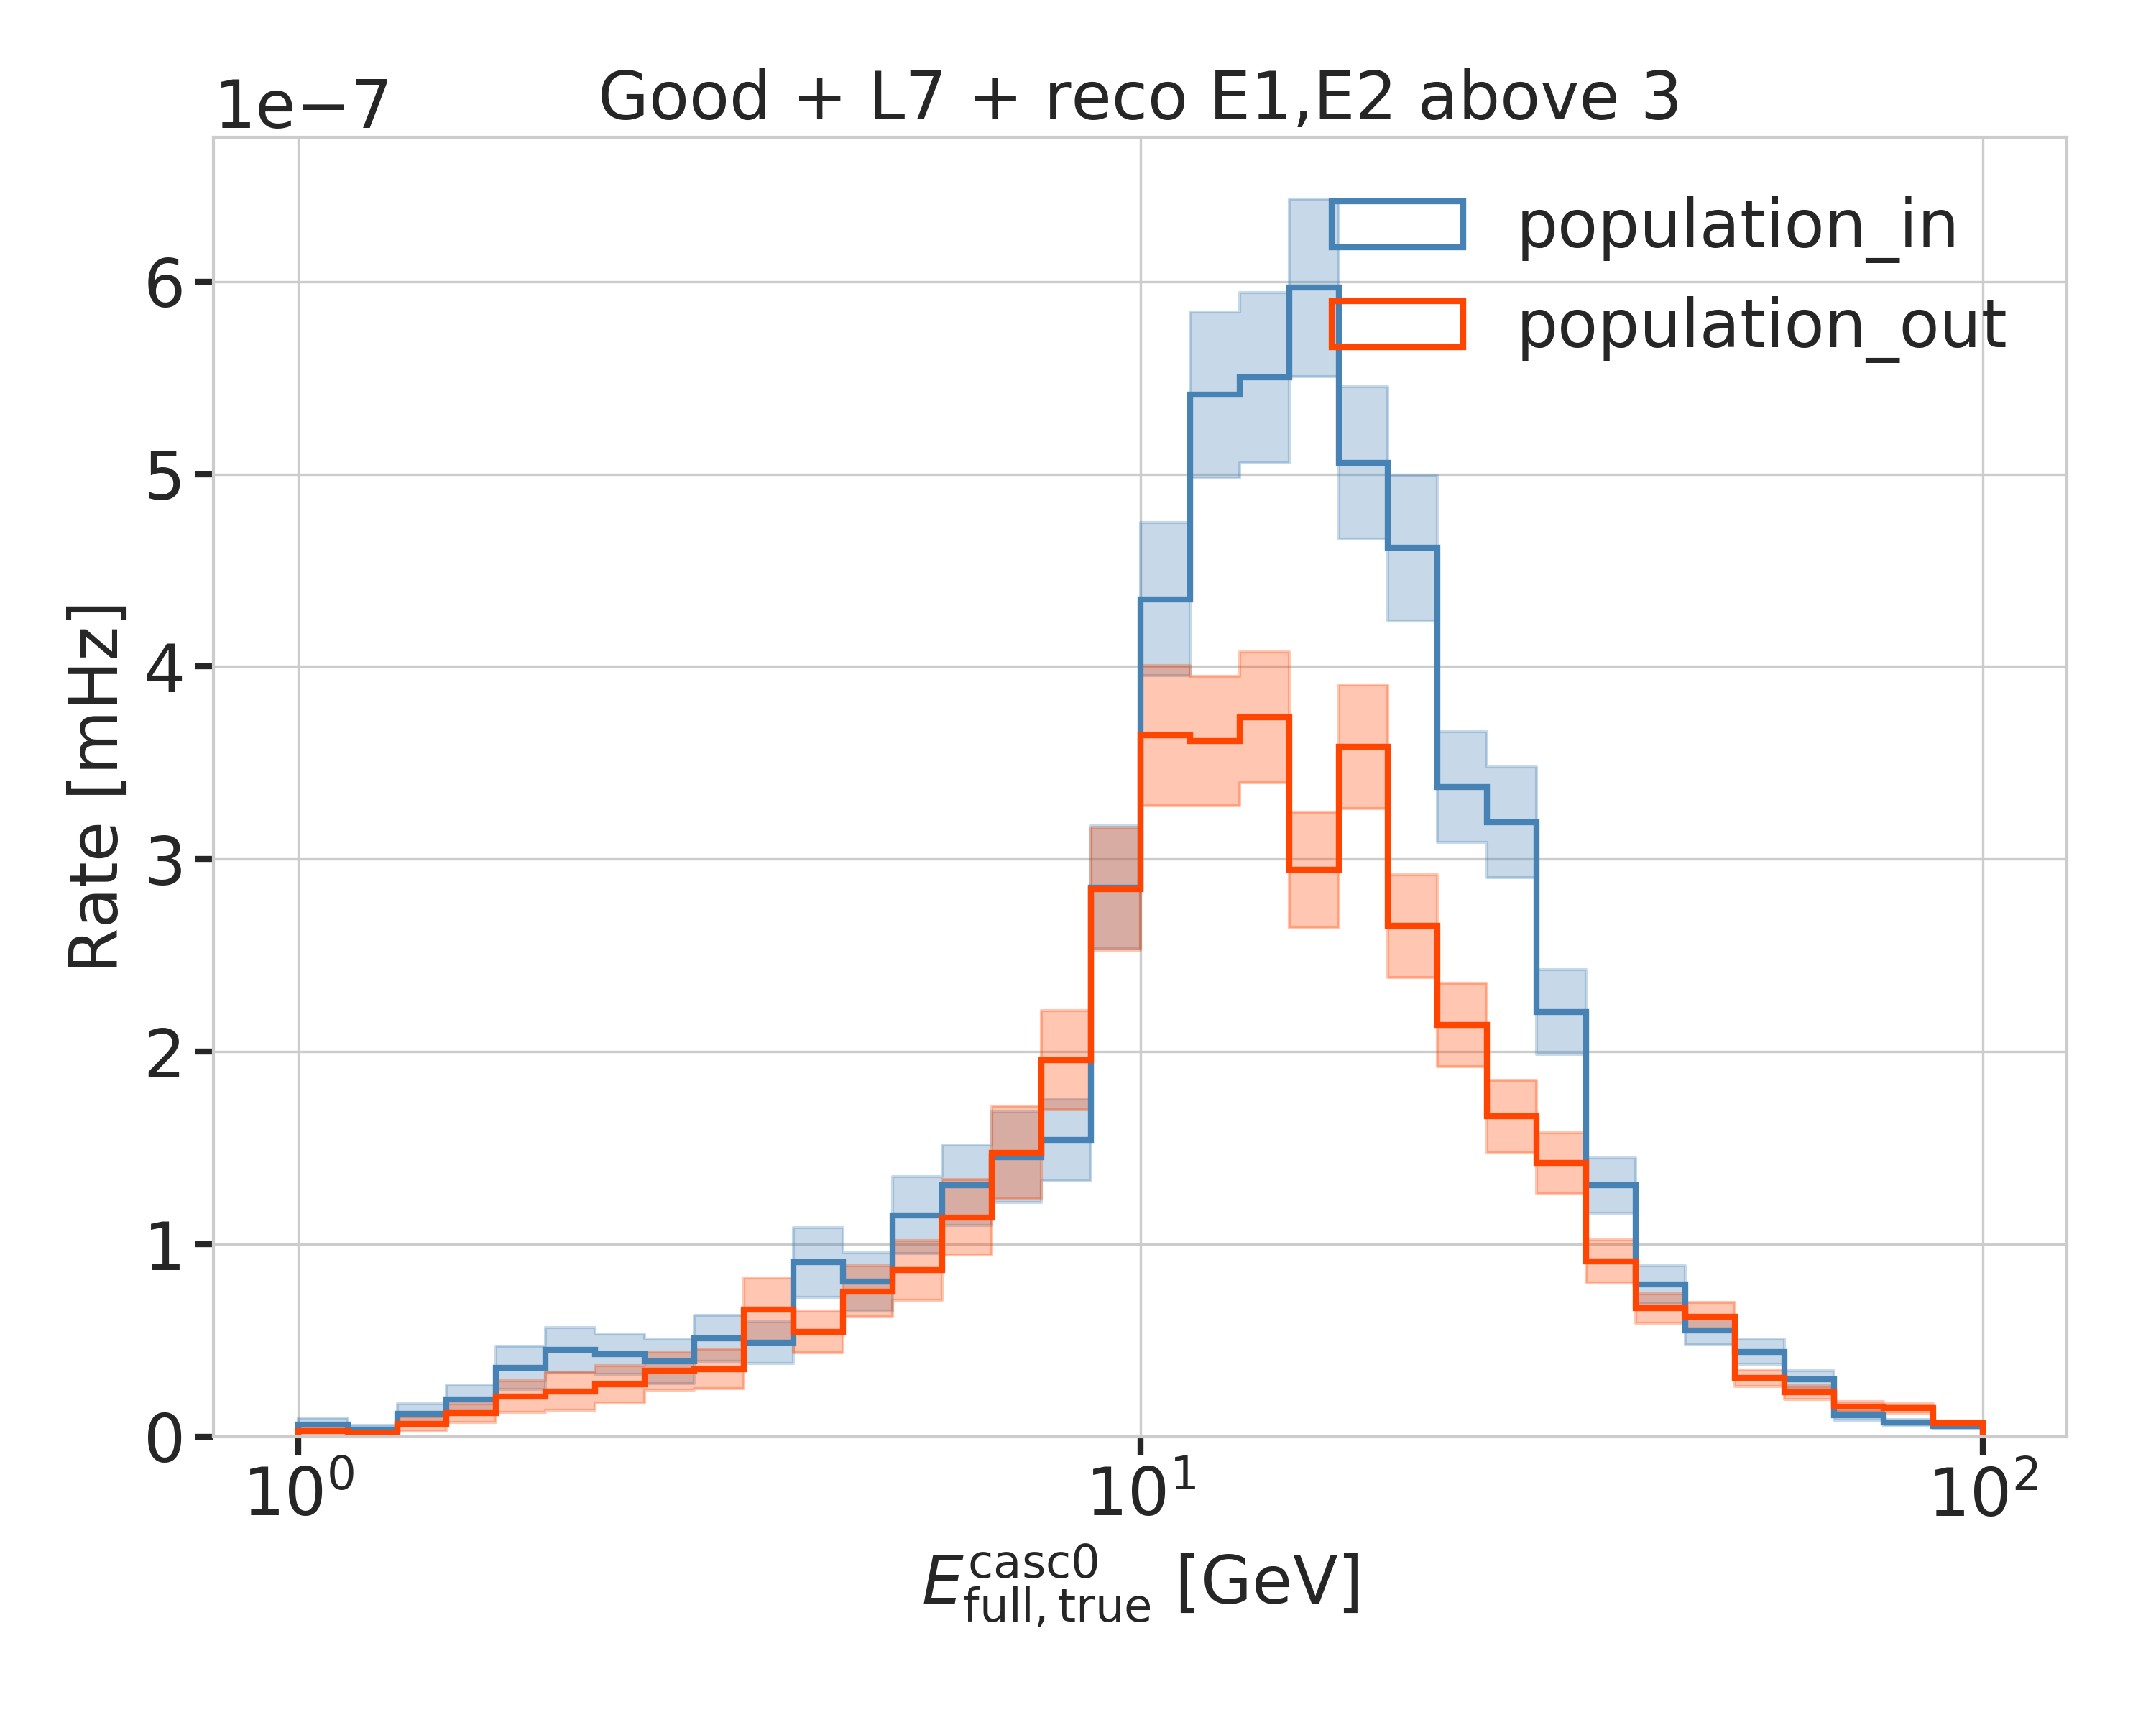
\includegraphics[width=0.49\linewidth]{figures/results/190607/second_population/casc0_energy.png}
    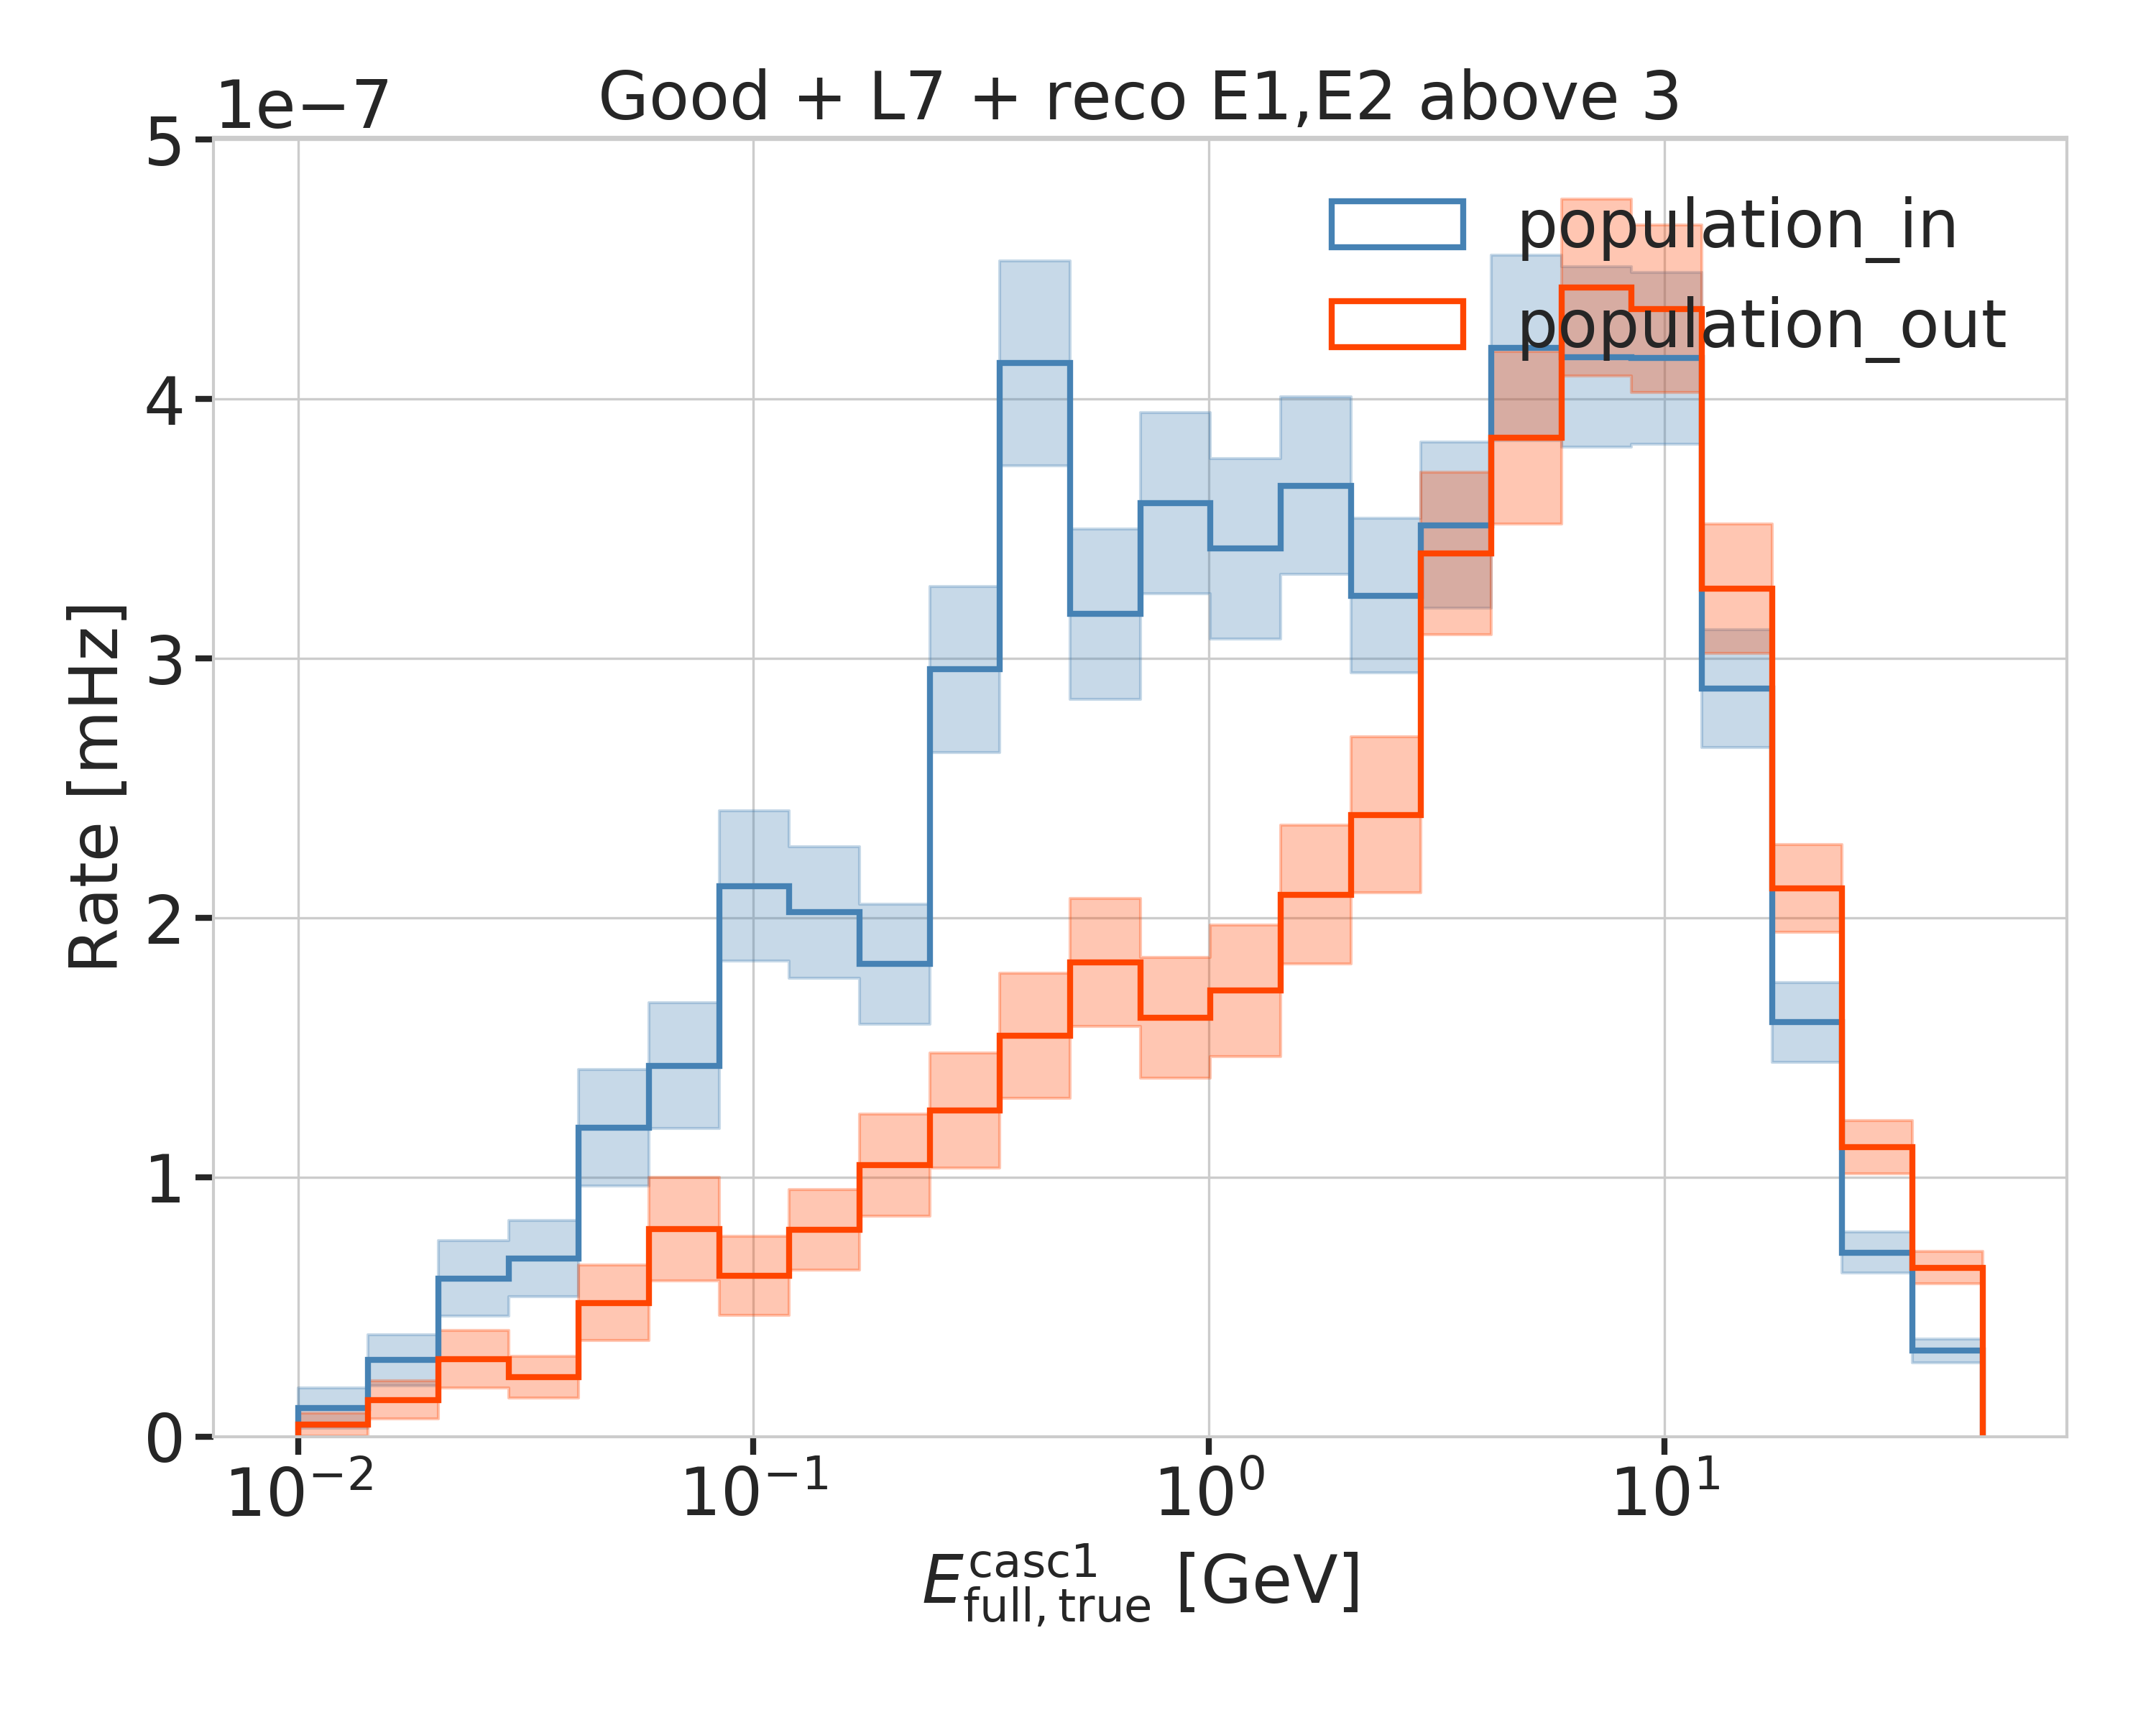
\includegraphics[width=0.49\linewidth]{figures/results/190607/second_population/casc1_energy.png}
    \caption[]{}
    \labfig{true_energies_vs_true_length}
\end{figure*}
\todo{re-make normalized? (ORANGE)}
\todo{fix caption (RED)}


\begin{figure*}[h]
    \centering
    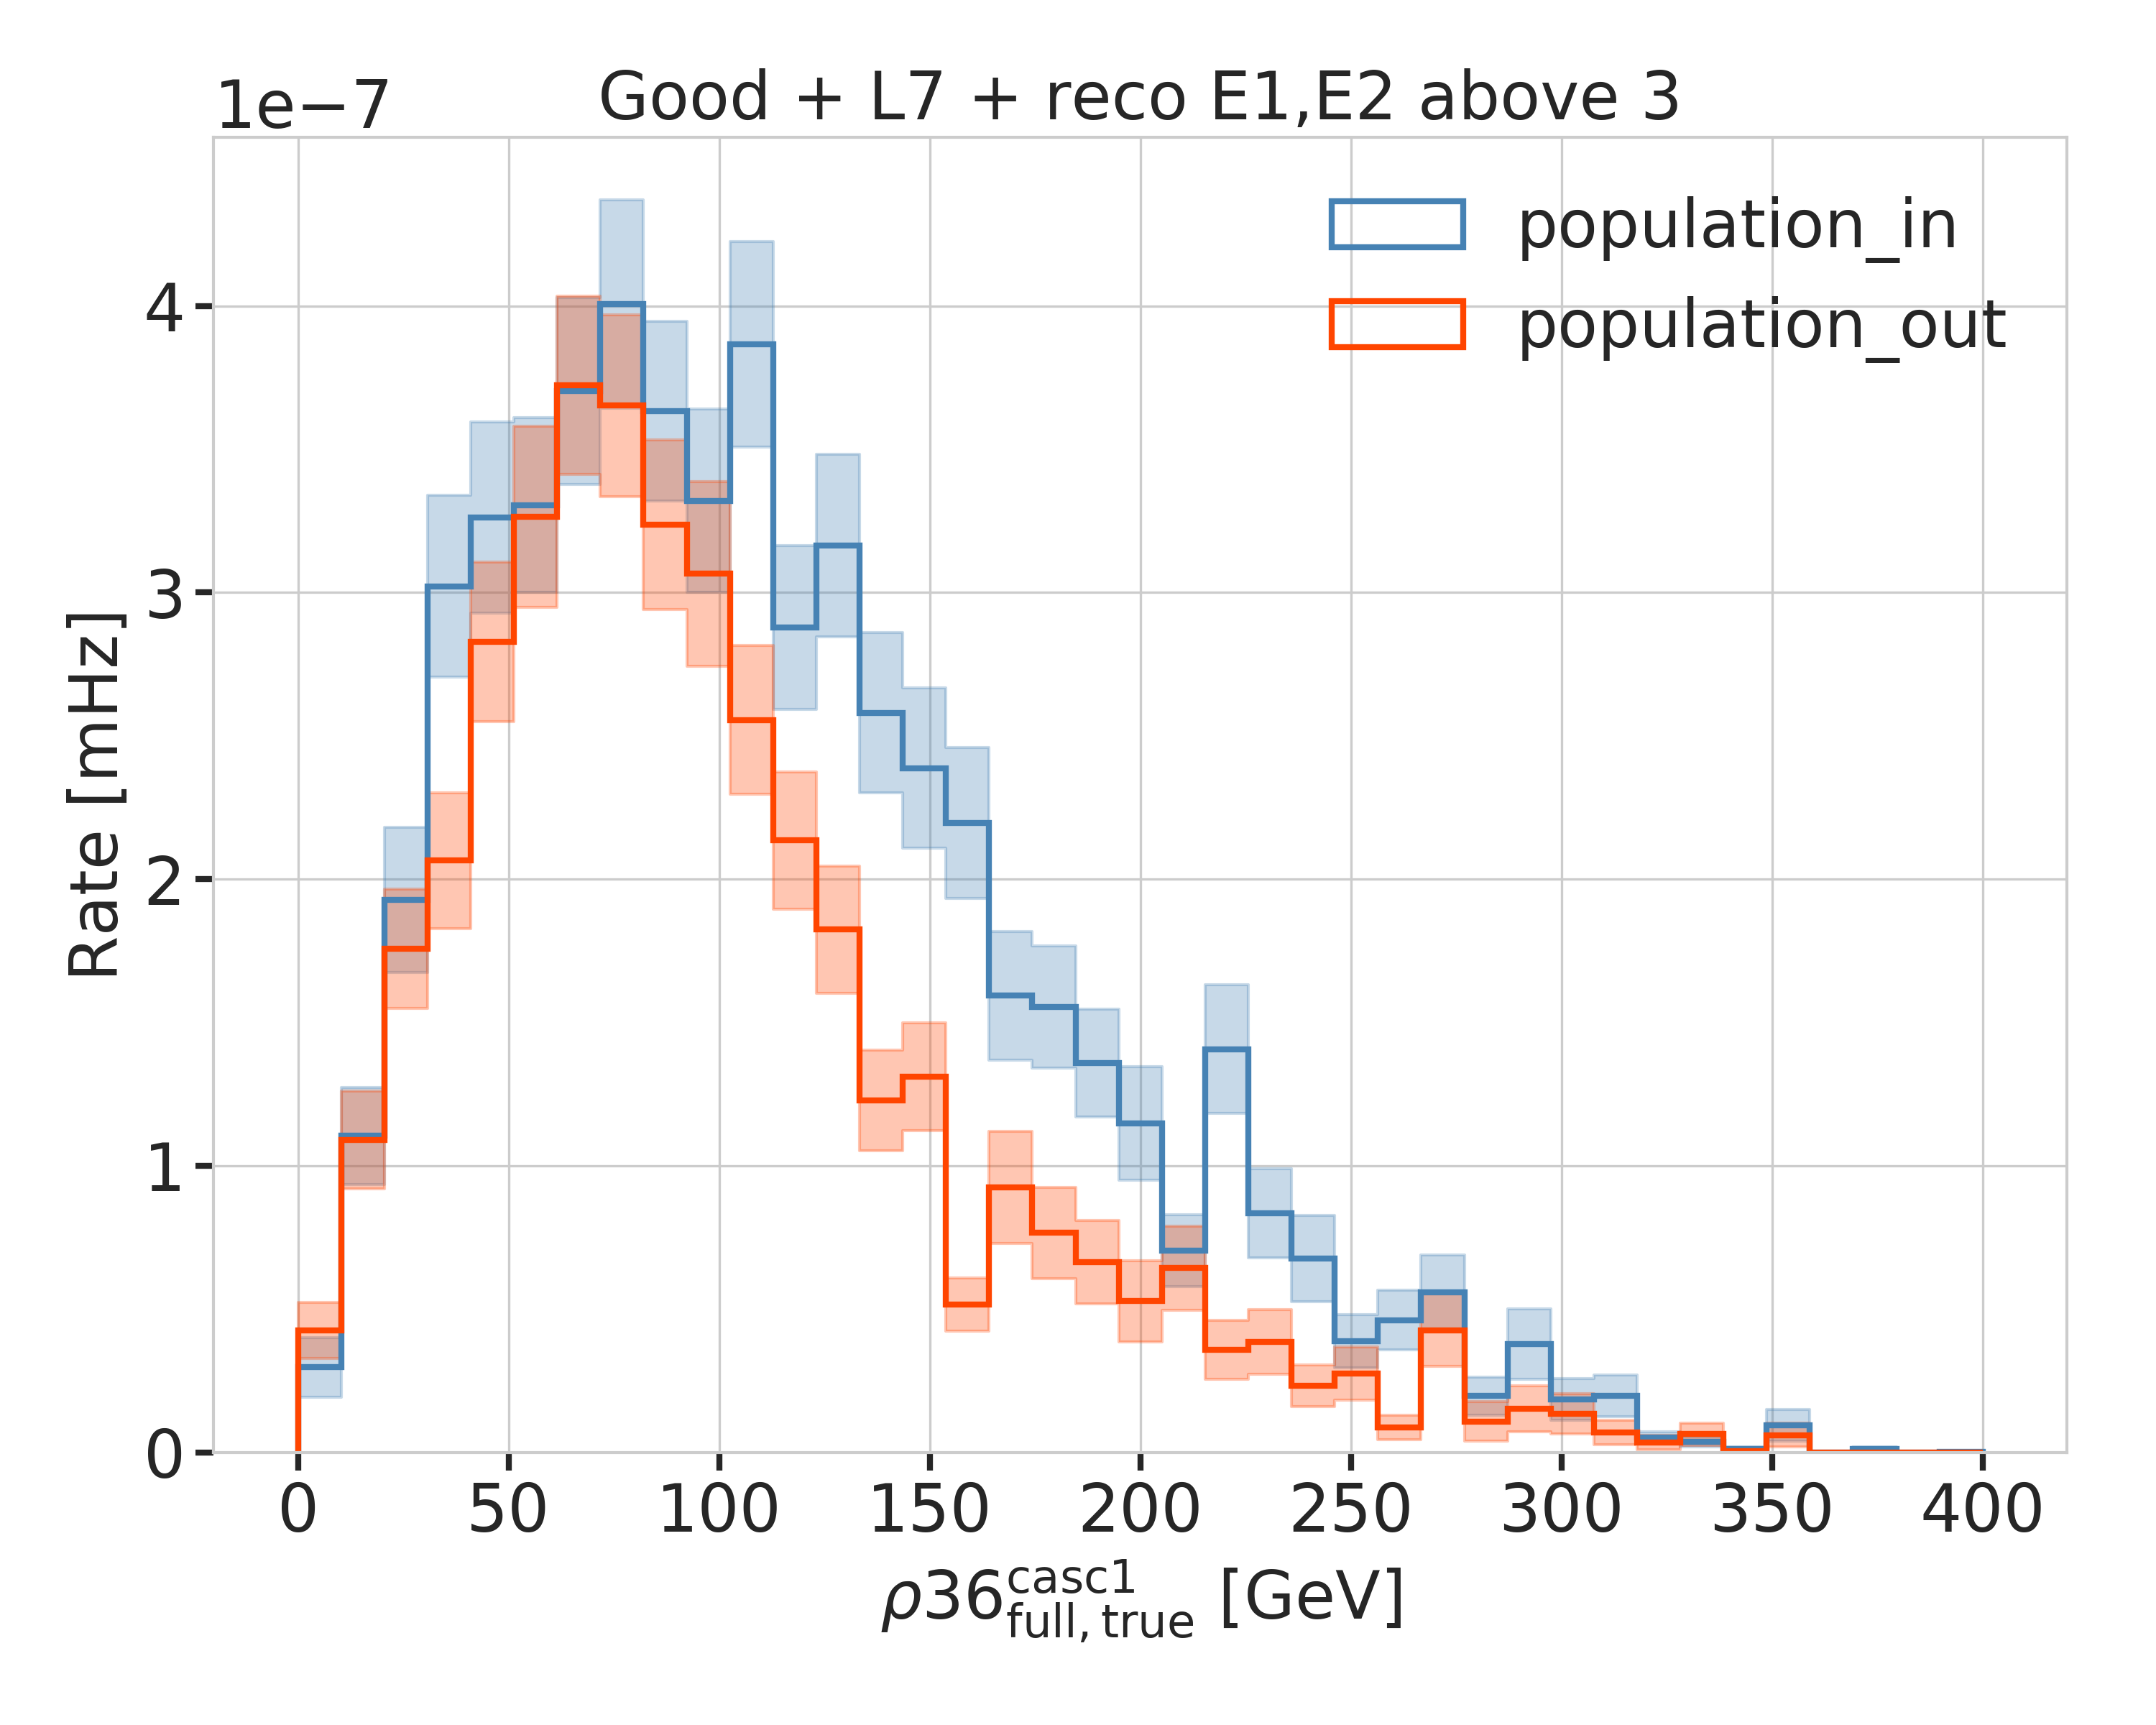
\includegraphics[width=0.49\linewidth]{figures/results/190607/second_population/casc1_rho36.png}
    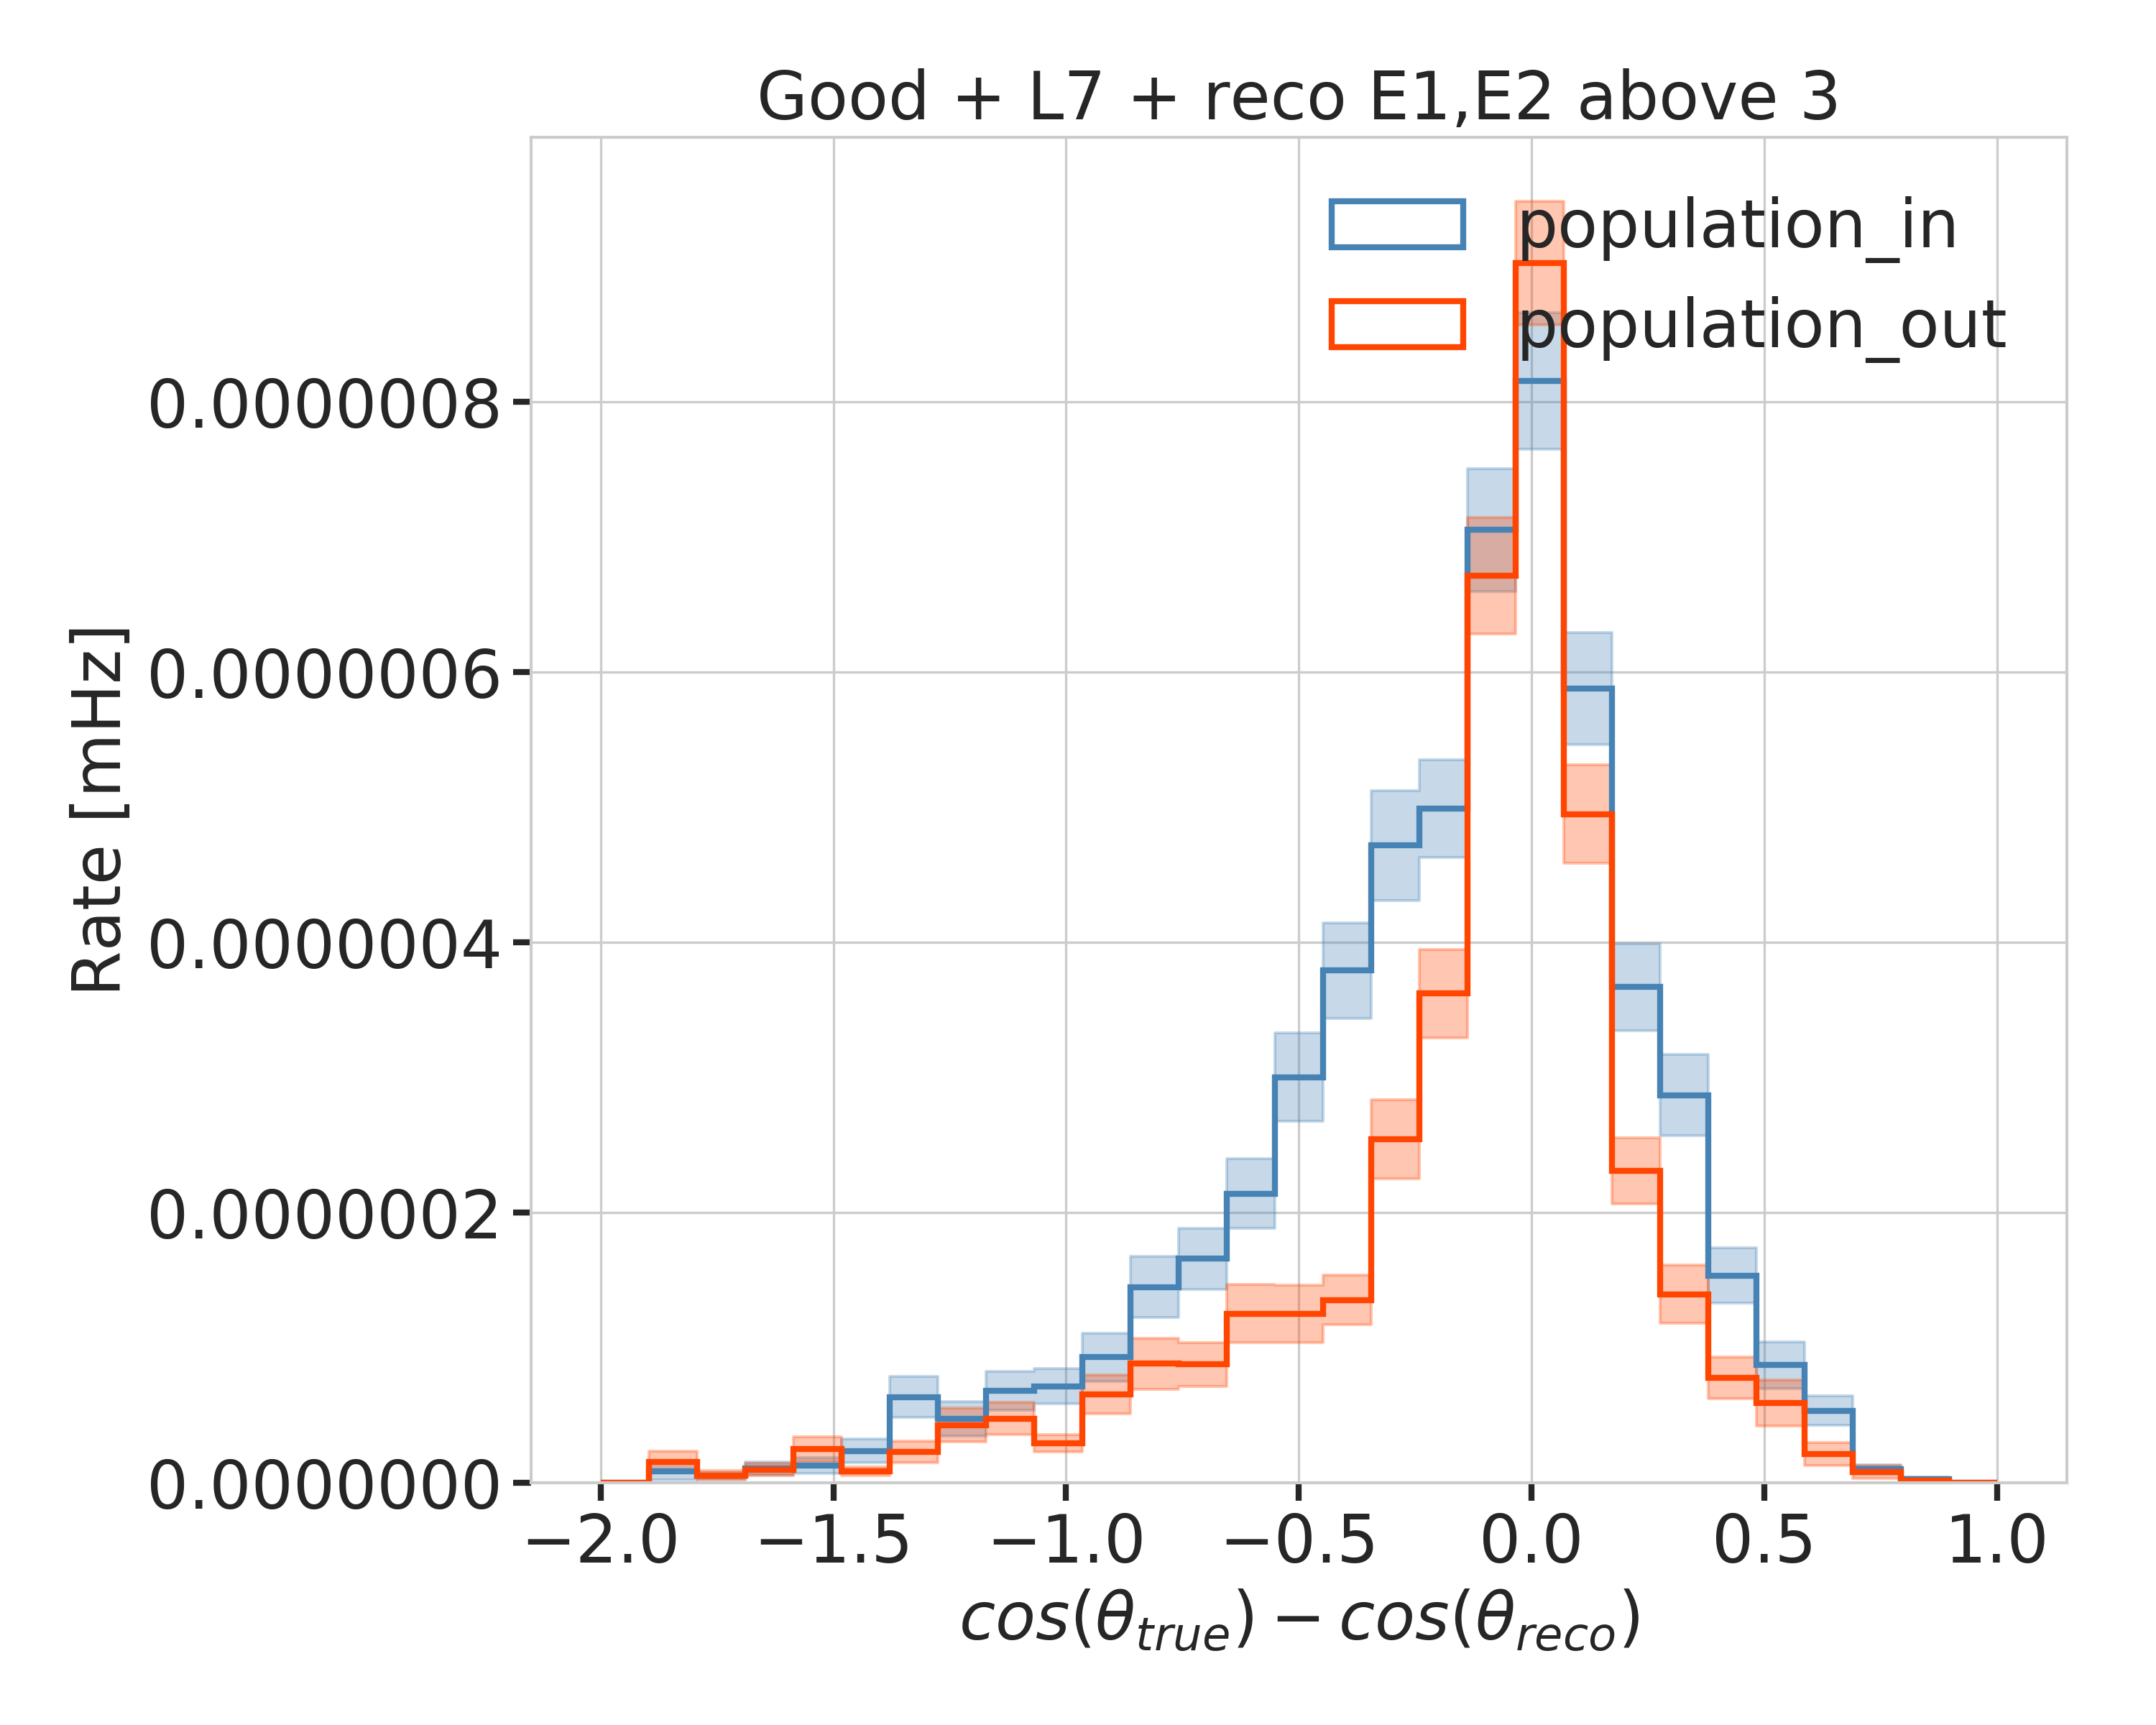
\includegraphics[width=0.49\linewidth]{figures/results/190607/second_population/reco_true_cos_zenith_error_populations.png}
    \caption[]{}
    \labfig{true_energies_vs_true_length}
\end{figure*}
\todo{re-make normalized? (ORANGE)}
\todo{fix caption (RED)}


\begin{figure*}[h]
    \centering
    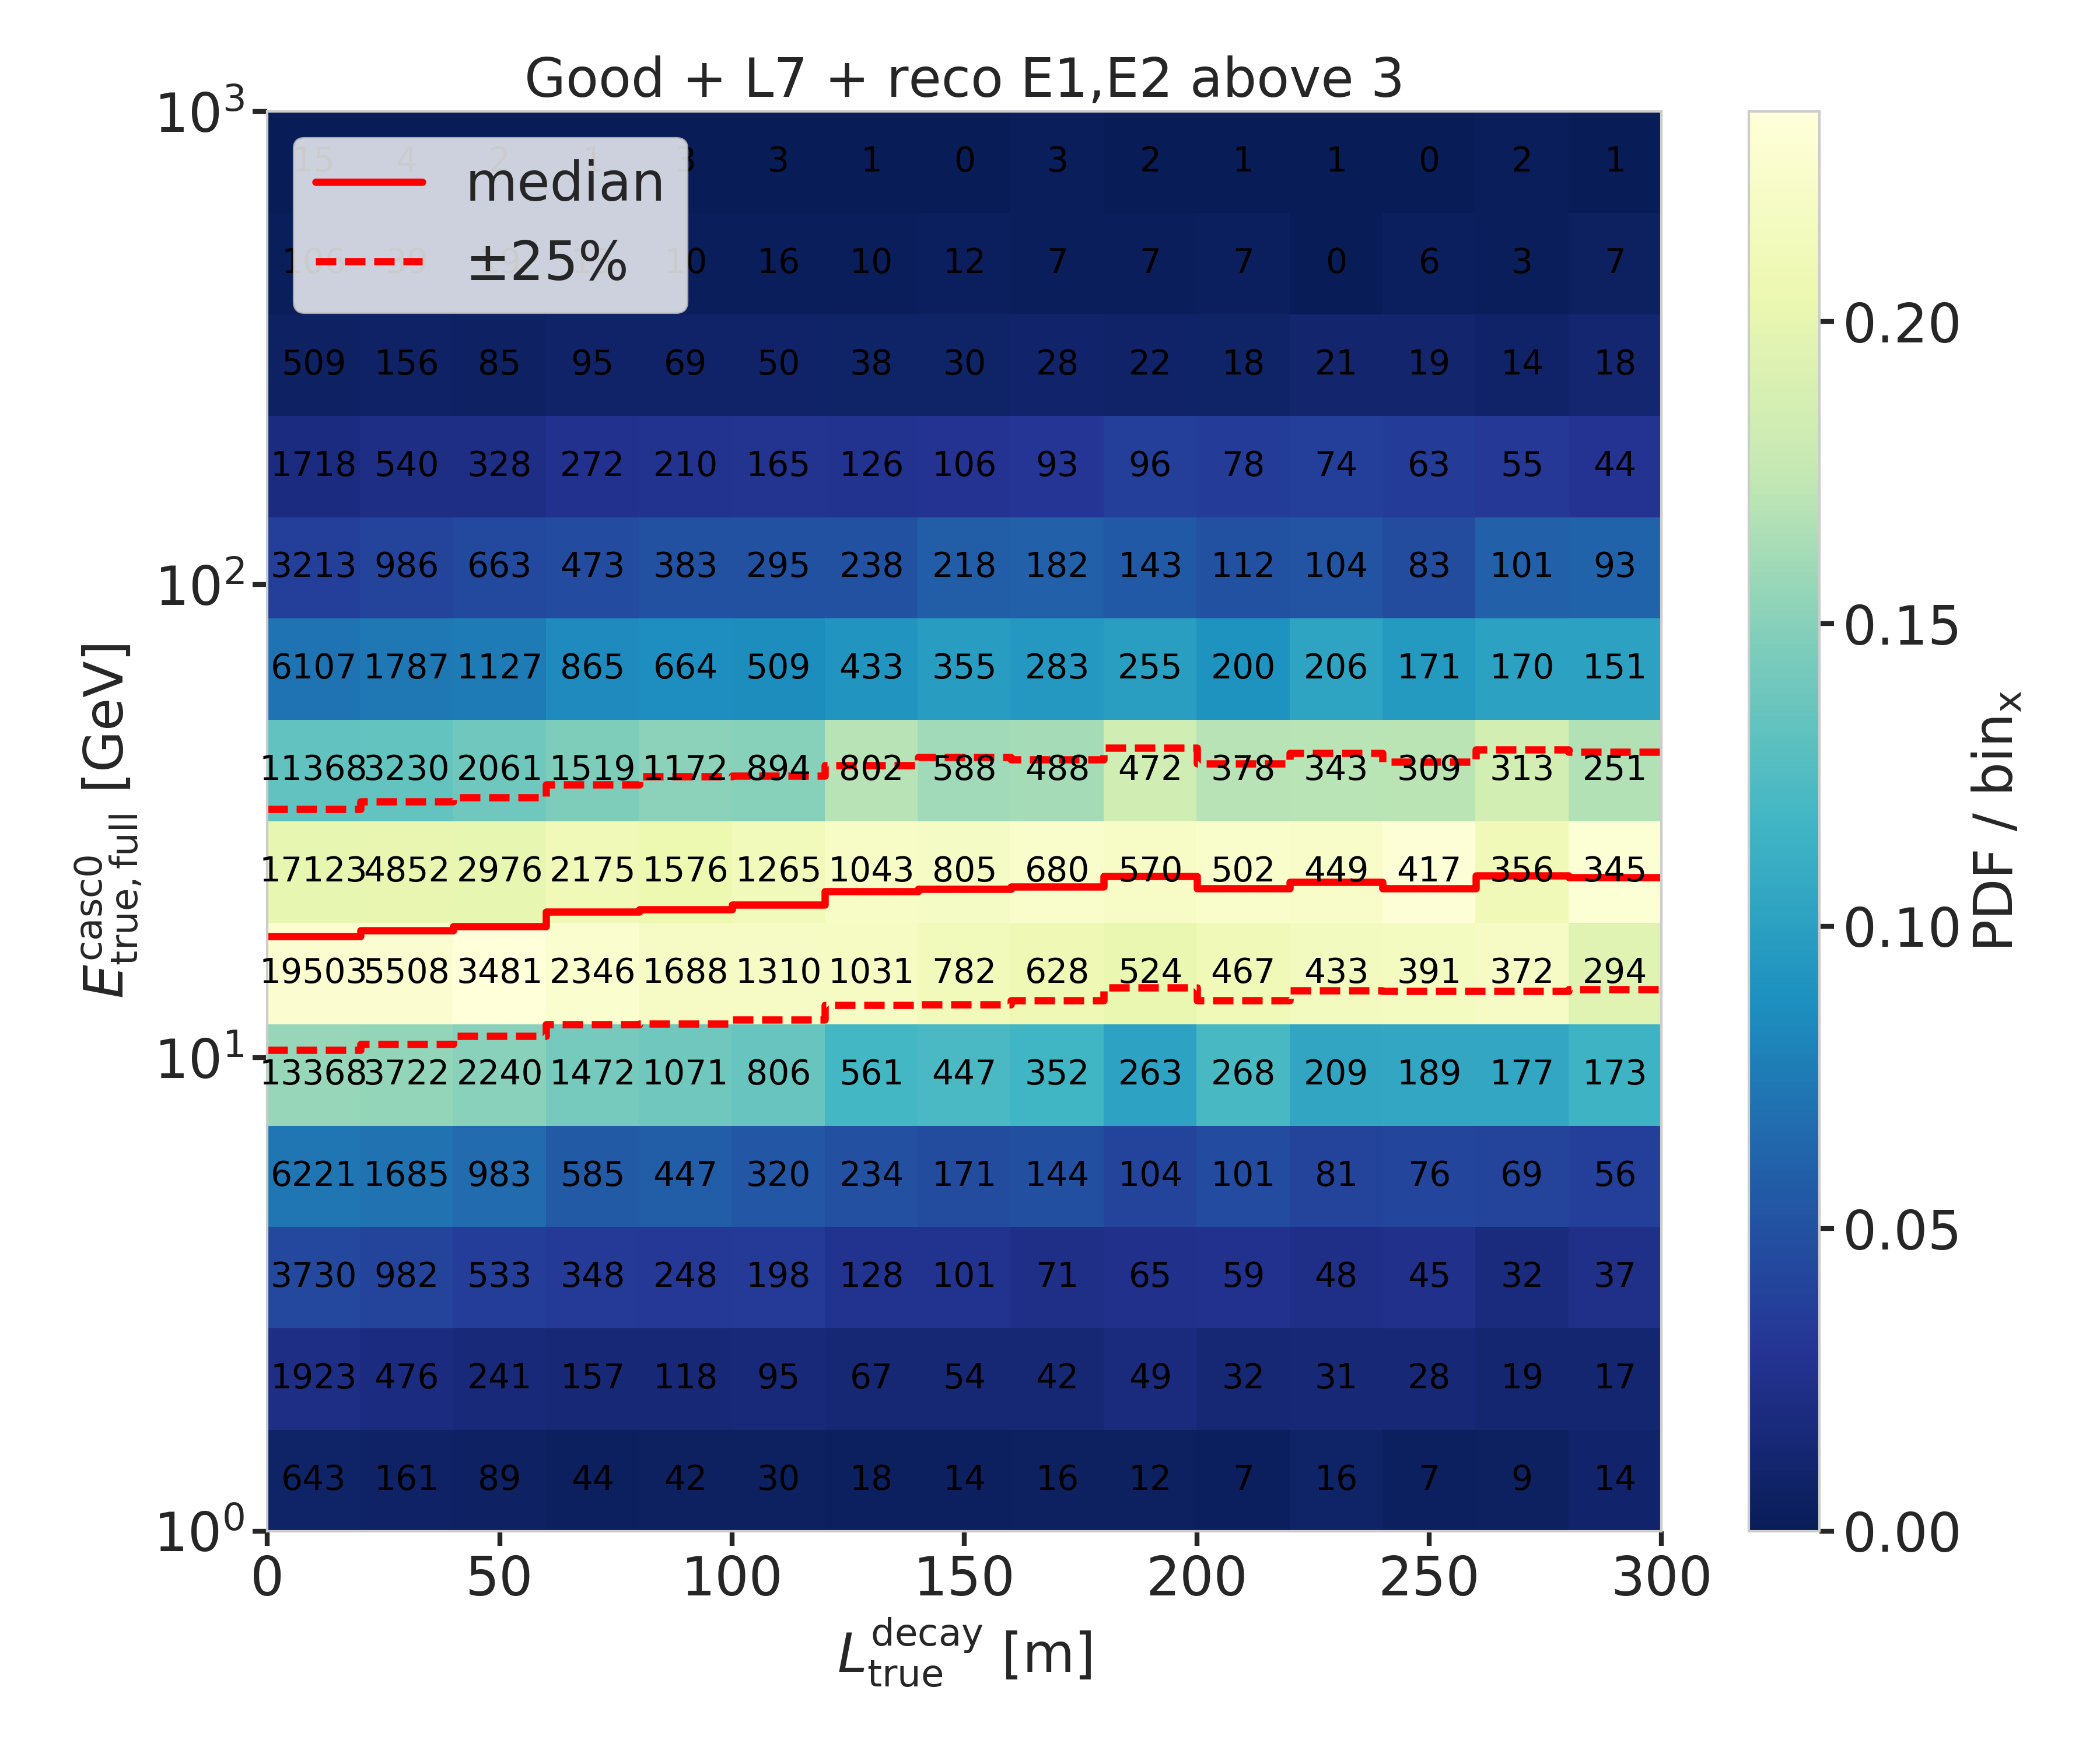
\includegraphics[width=0.49\linewidth]{figures/results/190607/true_decayL_vs_casc0_true_energy_reco_above3_step_contours.png}
    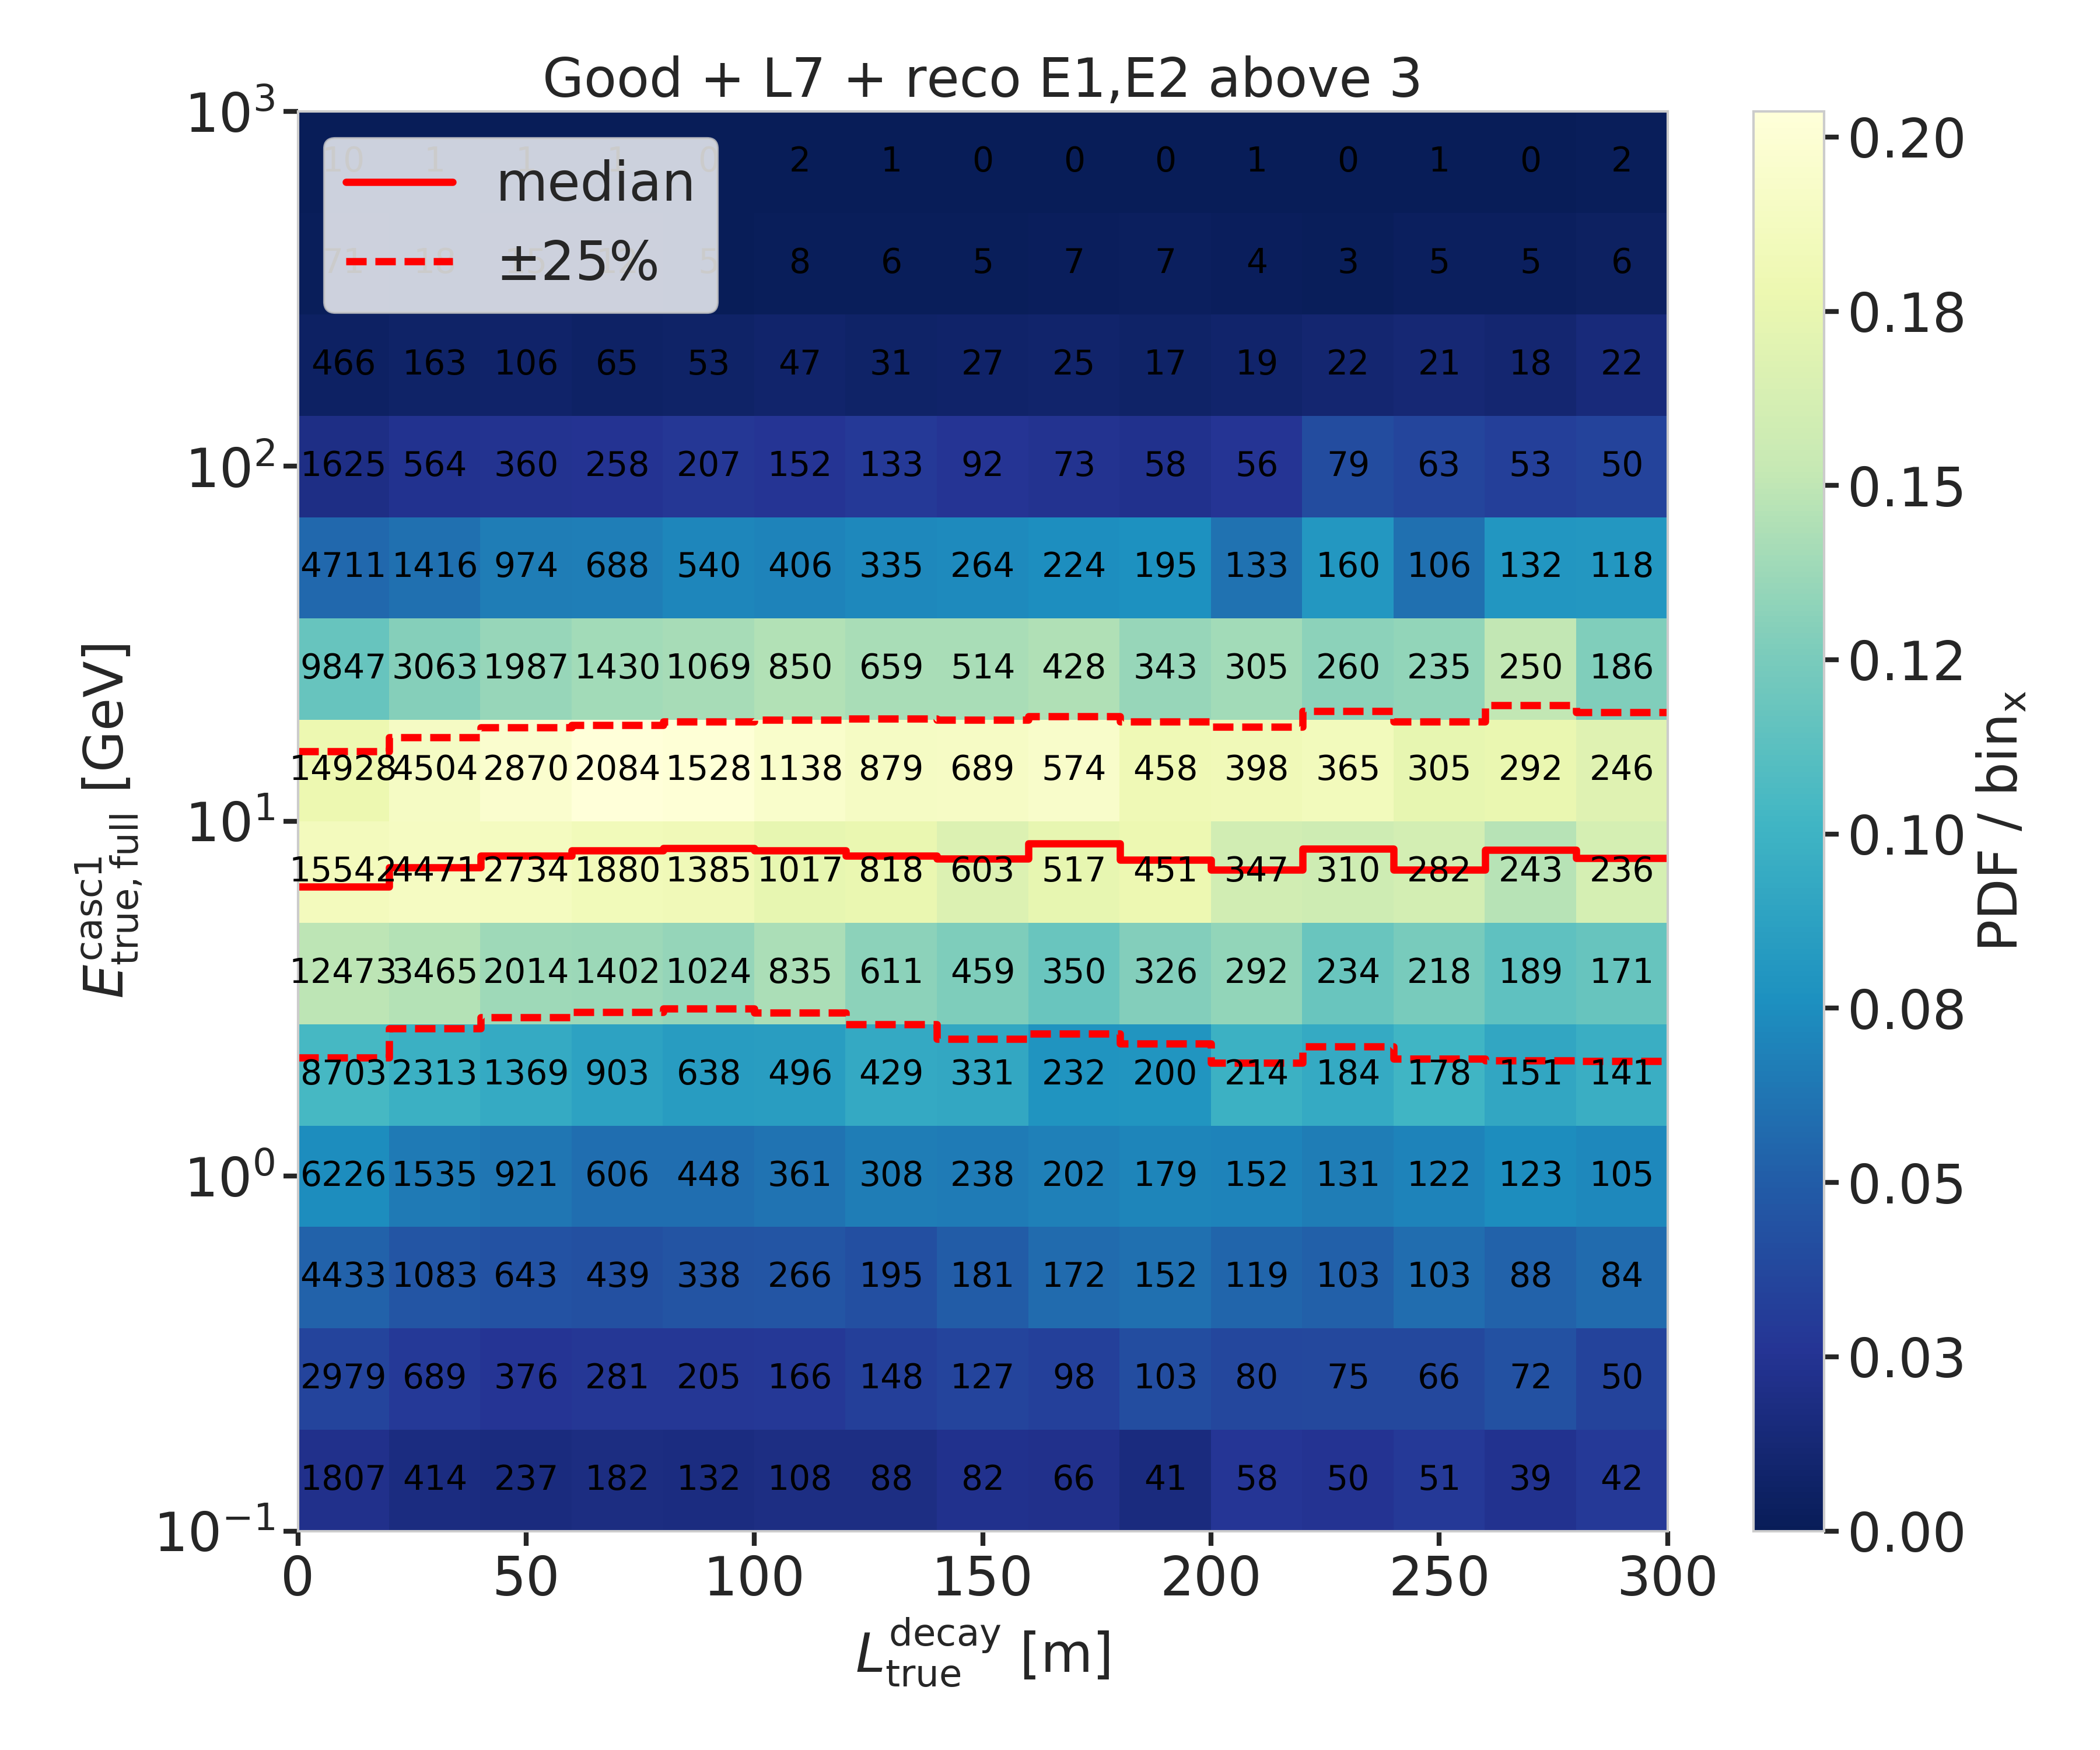
\includegraphics[width=0.49\linewidth]{figures/results/190607/true_decayL_vs_casc1_true_energy_reco_above3_step_contours.png}
    % \caption[Preliminary 2-d reconstructed versus true decay length resolutions]{Reconstructed decay length versus true decay length for a $\sim$\SI{3}{\gev} (left) and $\sim$\SI{10}{\gev} (right) minimum reconstructed cascade energies. The color scale is according to the PDF in each vertical true length slice, with the solid and dashed lines showing the median$\pm$\SI{25}{\percent} quantiles. The bin entries are shown as numbers.}
    \labfig{true_energies_vs_true_length}
\end{figure*}
\todo{fix caption (RED)}
\todo{I think from these plots it's probably enough if I state the median energy of first and second cascade at final level, as a benchmark for the energies of the two cascades (ORANGE)}


\section{Double Cascade Classification}

\paragraph{Missing Points}
\begin{itemize}
    \item Briefly mention MuMillipede "reconstruction" (depending on how deep I want to go into the classifier I tested?)
    \item Calculated variables to input the classifier (distributions?) I guess some examples might do?
    \item Cuts applied to make sure the classifier is trained on well reconstructed events (energy, length, true, reco..)
    \item Tested classifier (BDT) versions and their performance
    \item takeaway? (not sure how to deal with the caveat of the weight being kind of wrong for these..)
\end{itemize}


\section{Generic Double Cascade Performance}


\paragraph{Ideas:}
\begin{itemize}
    \item why do these checks again with the model independent samples? (controllable parameter space and distributions, especially energy and length)
    \item benchmark some edge cases (e.g. "best case" of up-going string centered, purely horizontal, and realistic case)
    \item investigate where the reconstructions breaks down (in terms of cascade energies, which are the main factor as shown before)
\end{itemize}

\subsection{Idealistic Performance}

\begin{itemize}
    \item for the perfect edge case of the event being directly on top of a DeepCore string with an up-going direction the length can be very well reconstructed above a true length of around \SI{20}{\meter}
    \item 2-d histogram shows that up to a true decay length of $\sim$\SI{210}{\meter}, there is no under-estimation of the length
    \item this means that the under-estimation observed before is only possible if there is no DOMs in between the two cascades
    \item this makes a lot of sense, since DOMs being present, but not observing any light is affecting the light expectation that goes into the reconstruction likelihood and therefore makes these hypotheses less likely and therefore incompatible with the data
    \item do I want more detailed plots here? I feel like this is enough.. 
\end{itemize}

\begin{figure*}[h]
	\centering
    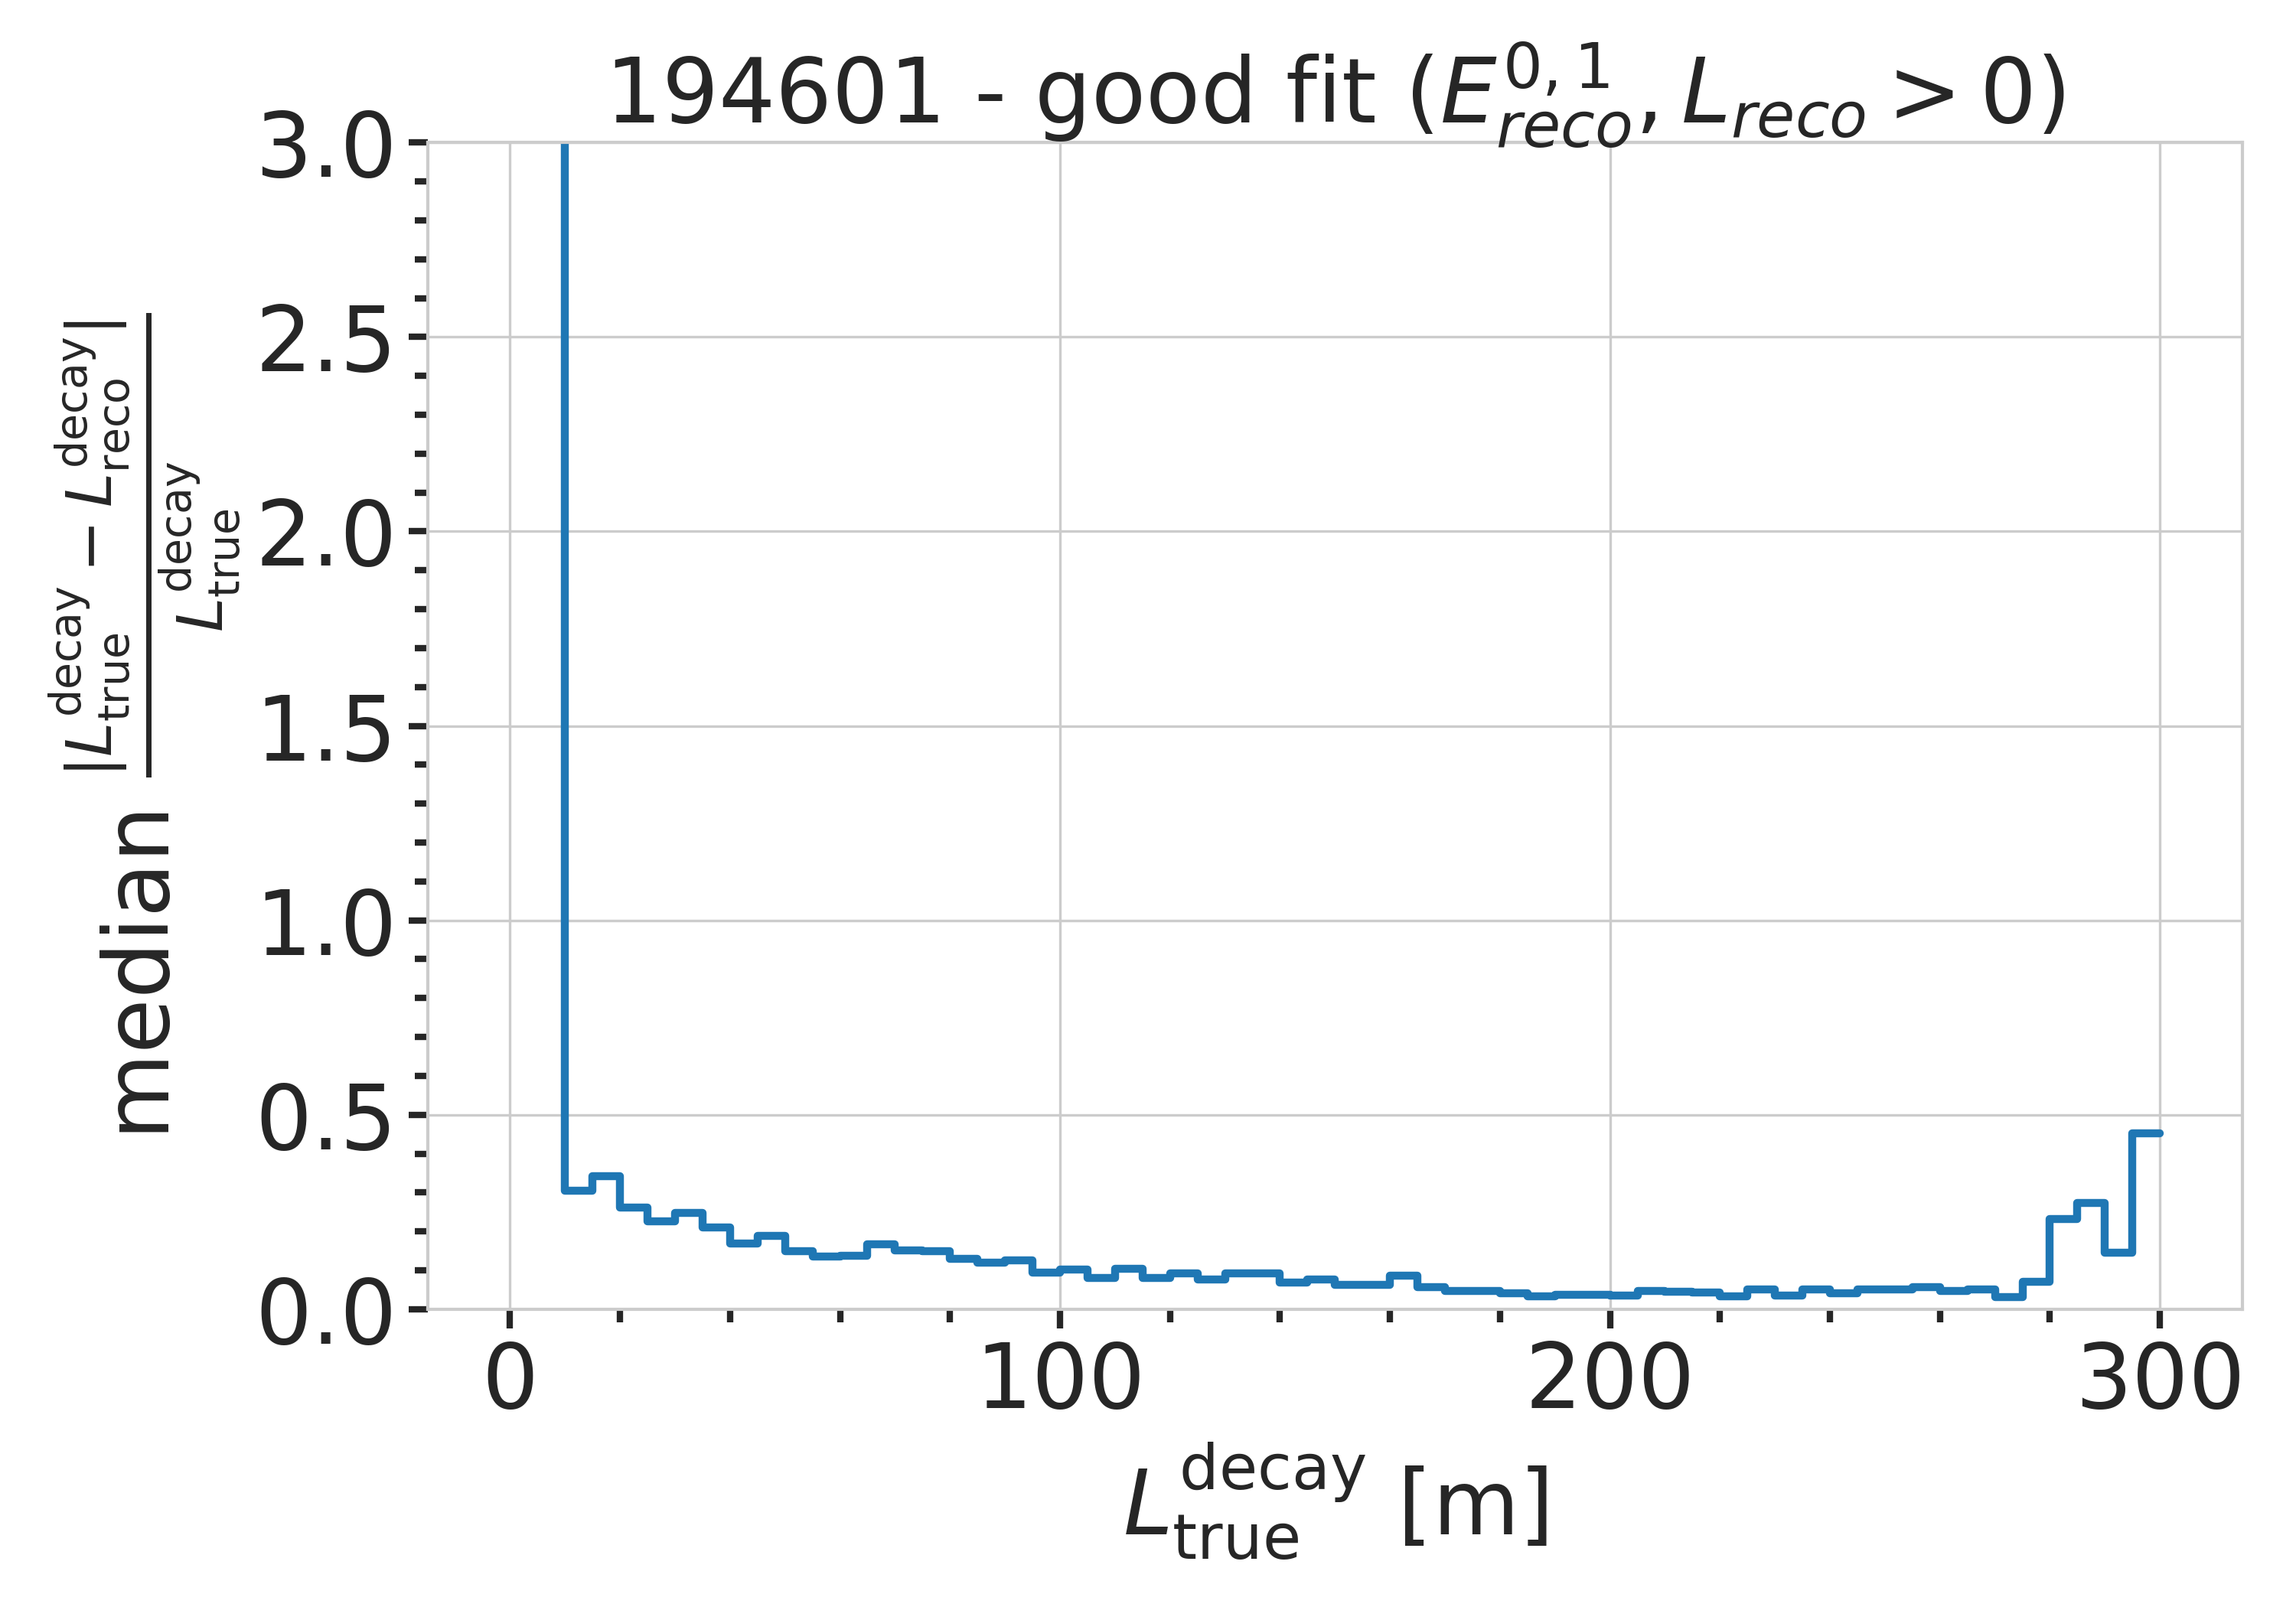
\includegraphics[width=0.49\linewidth]{figures/model_independent_simulation/results/idealistic/194601_median_decay_length_resolution_goodfit_log_unweighted.png}
    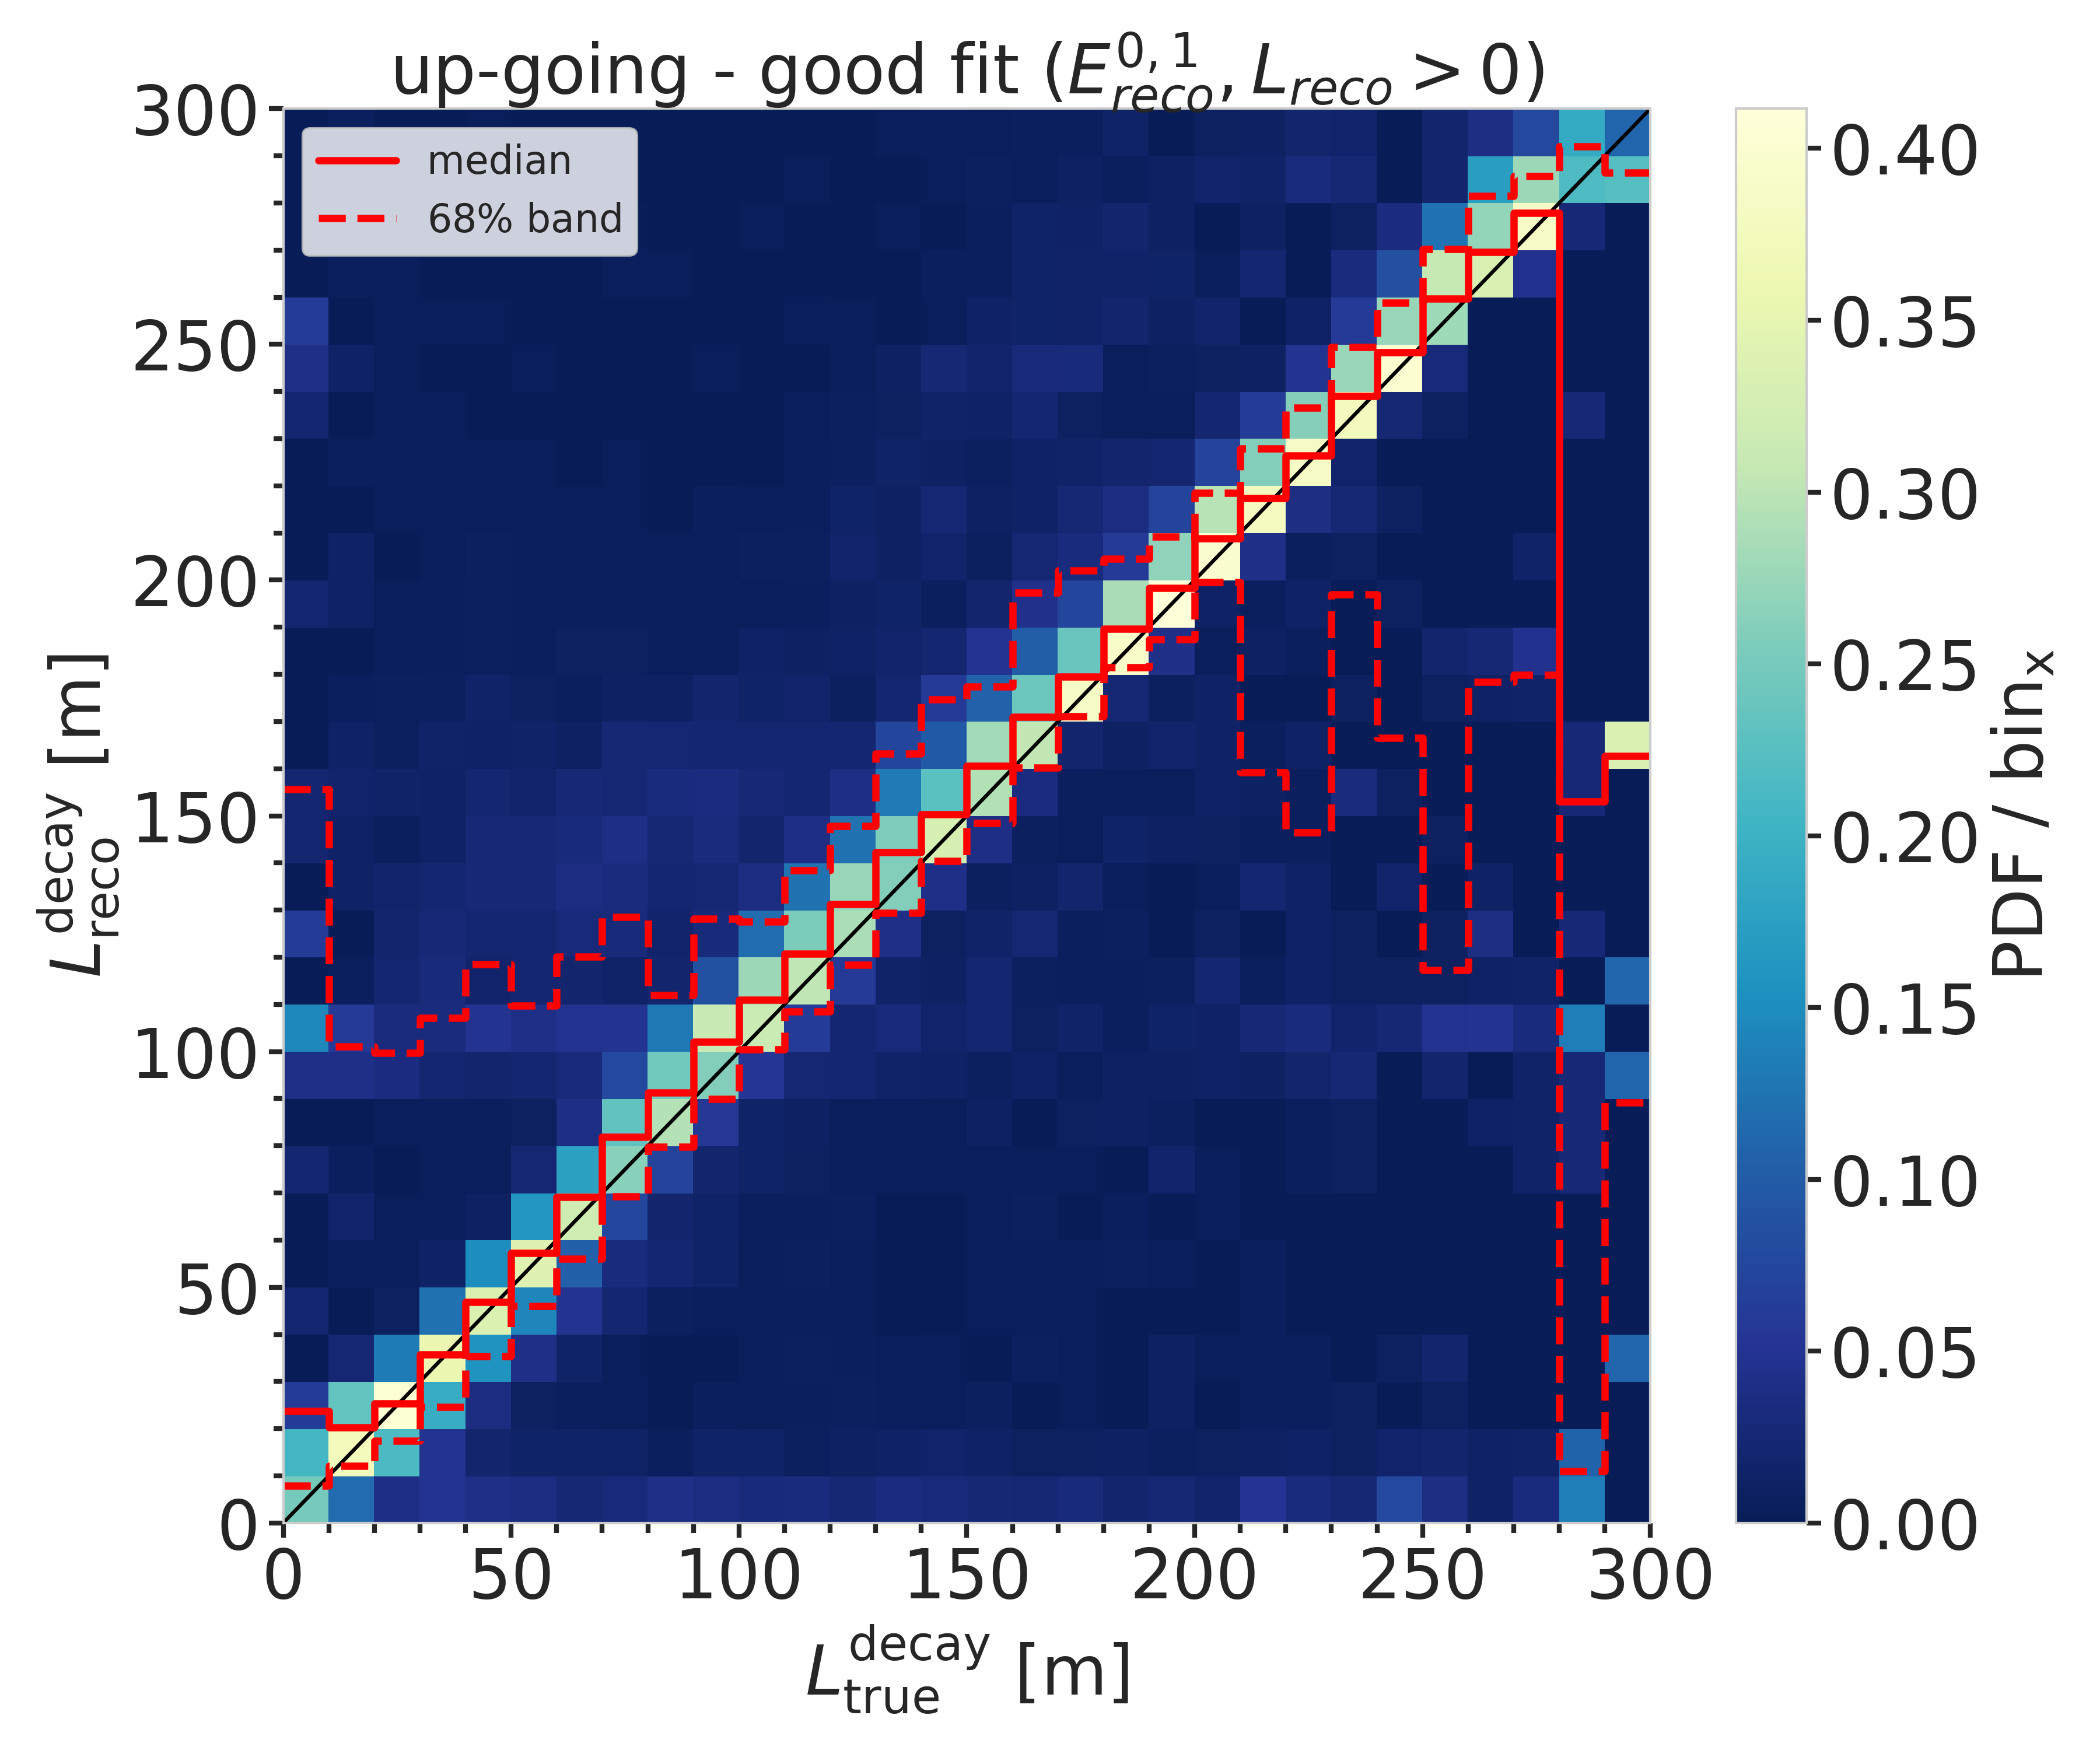
\includegraphics[width=0.49\linewidth]{figures/model_independent_simulation/results/idealistic/194601_reco_decay_length_vs_true_decay_length_goodfit_step_contours.png}
    \caption[]{}
    \labfig{idealistic_length_resolutions}
\end{figure*}
\todo{fix caption of this figure (RED)}



\subsection{Realistic Performance}

\subsubsection{Energy/Decay Length Resolution}

\todo{describe the "good fit" selection when I first show plots that use it (ORANGE)}
\todo{add some 1D resolution plots (ORANGE)}

\subsubsection{2-D Histograms}

\textbf{Things to mention about the 2d-hists:}
\begin{itemize}
    \item total energy resolution looks very good, above \SI{10}{\gev} it's almost unbiased and the 1-sigma resolution band is below \SI{20}{\percent}
    \item individual cascade resolutions mirror this behavior, but are starting to stabilize in energy at lower energies around \SIrange{5}{6}{\gev} with a broader resolution band of \SI{50}{\percent}, but reducing drastically with increasing energy (down to \SI{20}{\percent} at \SI{100}{\gev})
    \item interestingly, the second cascade energy reconstruction performs slightly worse, although they have the same energy ranges. This could hint at an asymmetry in the reconstruction process (might relate to how the two cascades are parameterized) or be due to the different positions and the dominantly up-going direction used in the sampling combined with the DOMs looking down (relate this to the sampling distribuitons explained/shown in the previous chapter)
    \item the decay length resolution looks much worse. In the region between \SIrange[range-phrase={~and~}]{20}{80}{\meter} it's roughly unbiased, but 1-sigma resolution band is quite wide with a lot of outliers towards short reconstructed lengths. Below \SI{20}{\meter} the reconstructed lengths are always over-estimating the true and above \SI{80}{\meter} a population of events start to dominate where the decay lengths isn't getting reconstructed at all, which might indicate that one of the cascades wasn't observers. (Relate to the fact that this marginalizes over all energies, meaning also all events which have one cascade with very low energy are included here.)
    \item another interesting feature is the band of reconstructed lengths around \SI{100}{\meter}, which is probabaly related to the spacing between most of the strings, which favors the reconstruction to be around this value, because that's the distance at which light can be observed, just from the fact that the DOMs are spaced at this distance (for low energetic cascades, this can dominate the reconstruction)
\end{itemize}


\begin{figure*}[h]
	\centering
    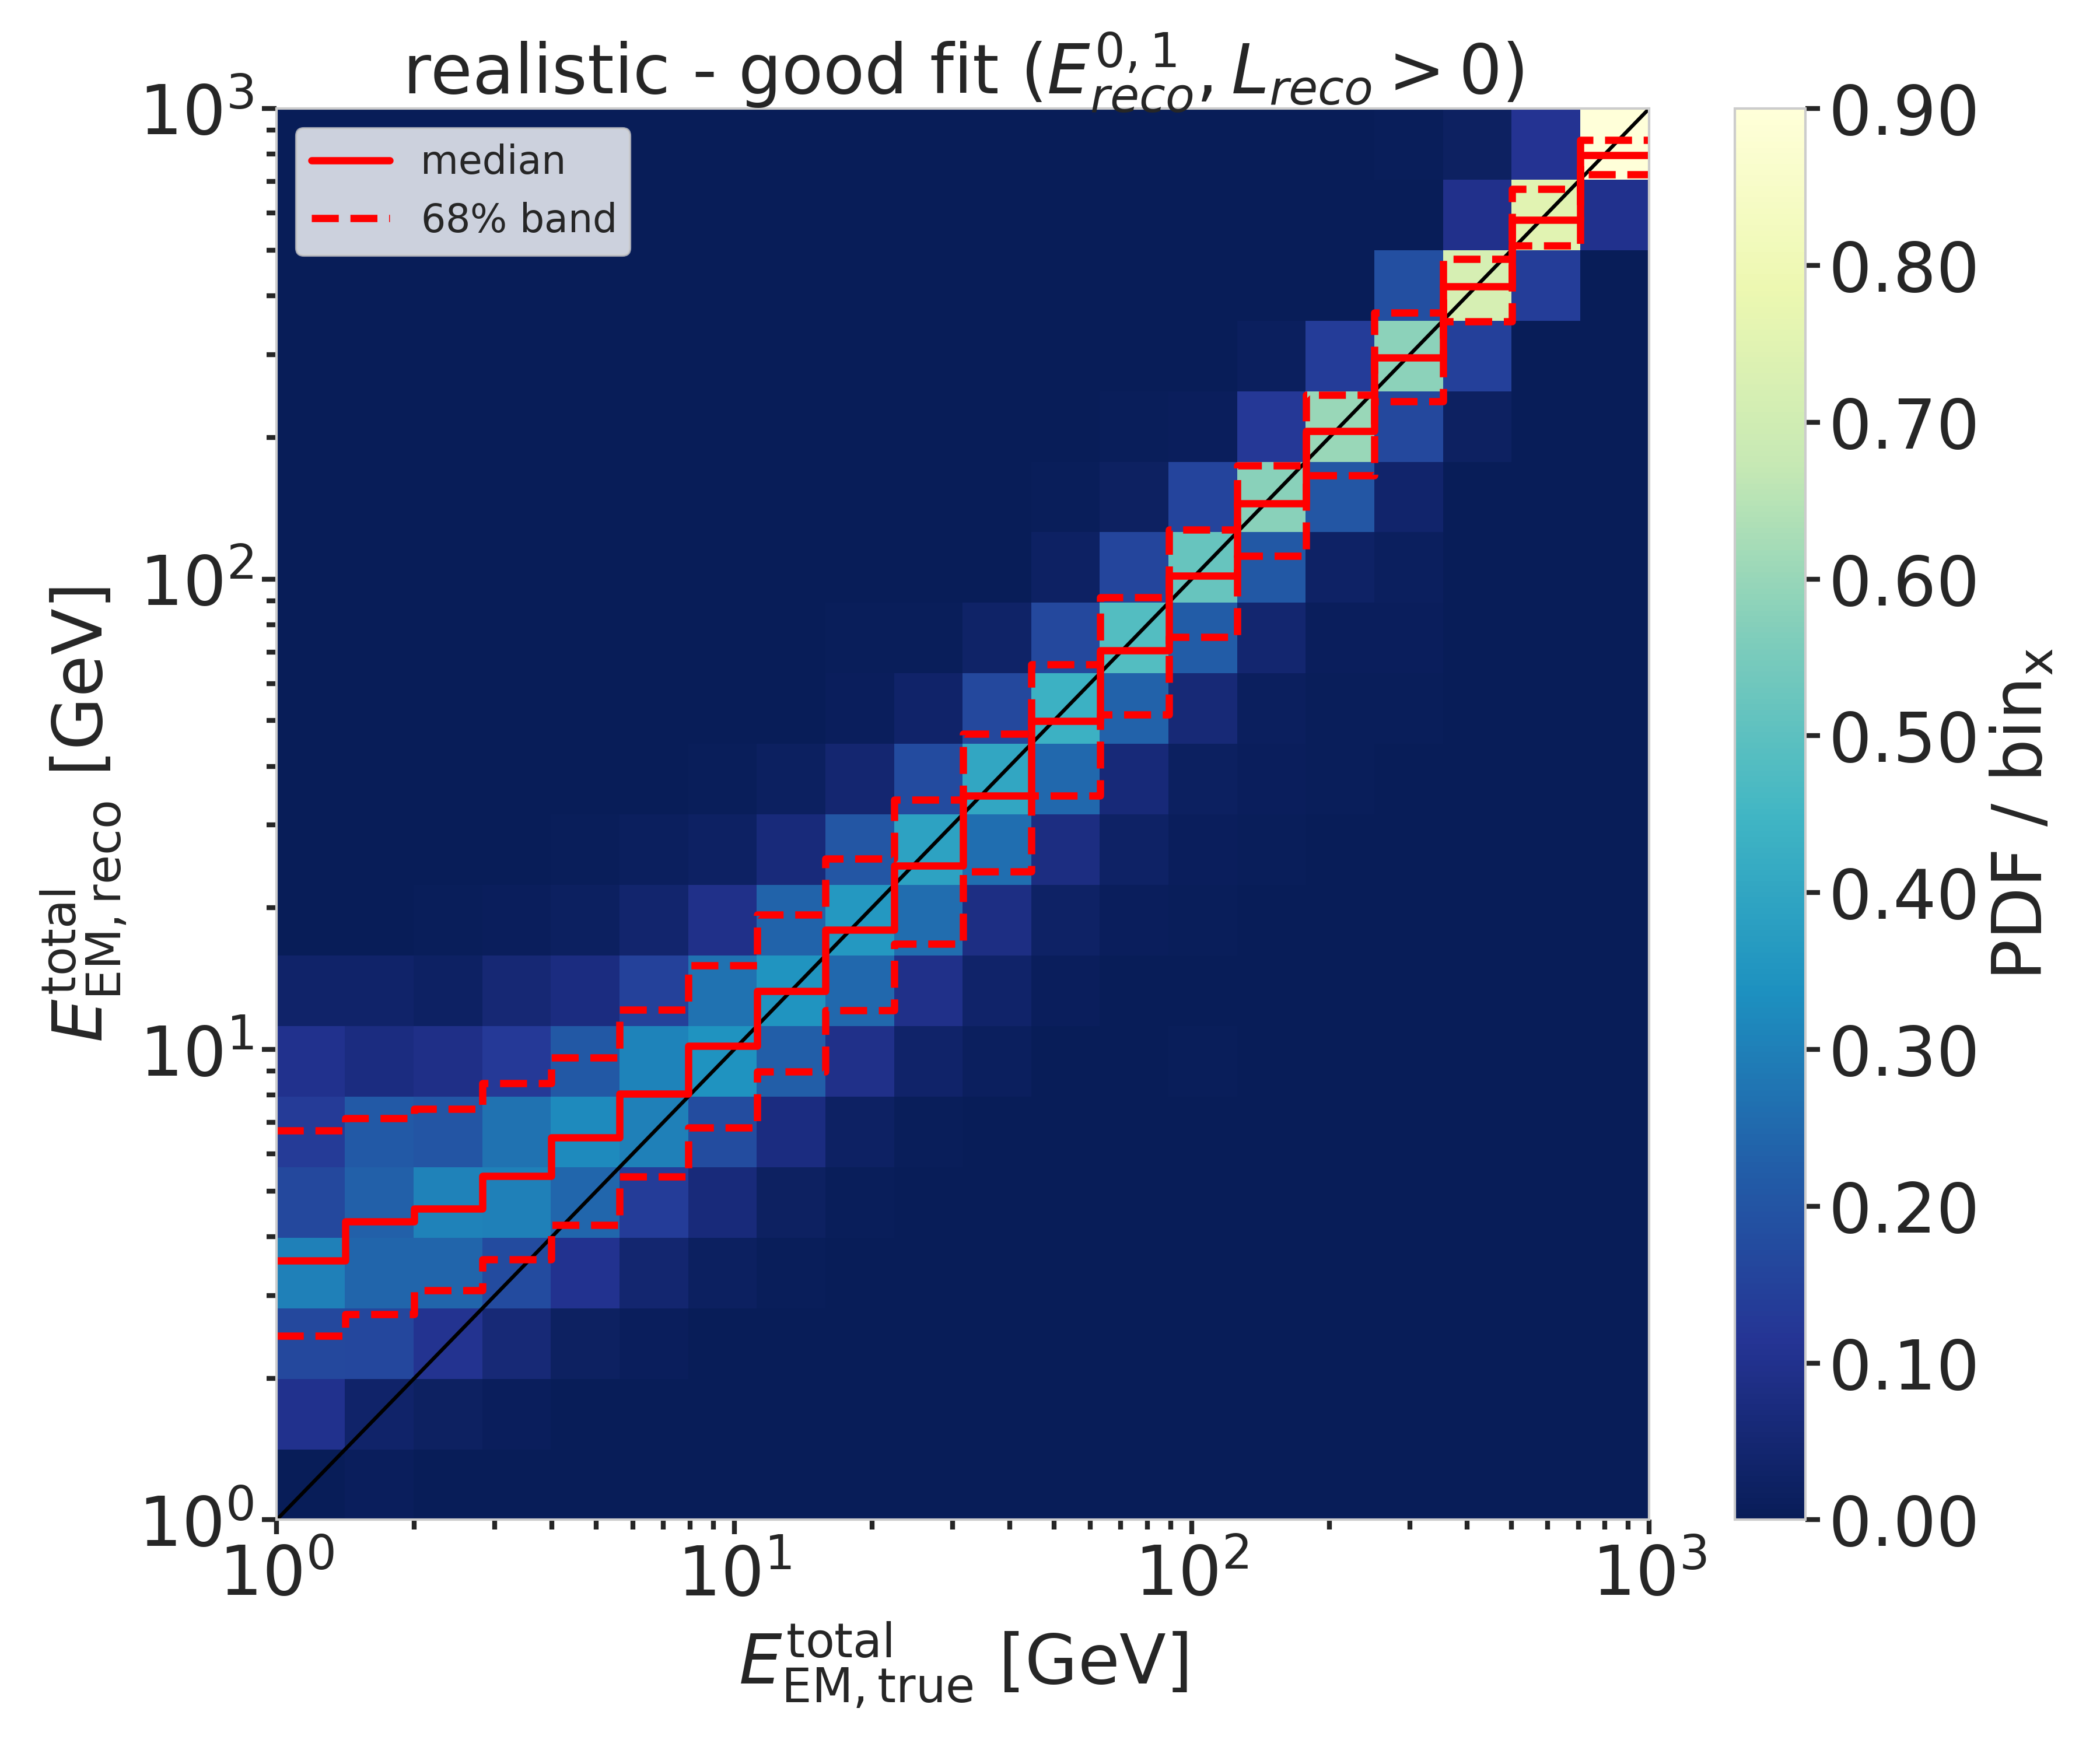
\includegraphics[width=0.49\linewidth]{figures/model_independent_simulation/results/realistic/2d_hists/194603_reco_total_energy_vs_true_total_energy_goodfit_step_contours.png}
    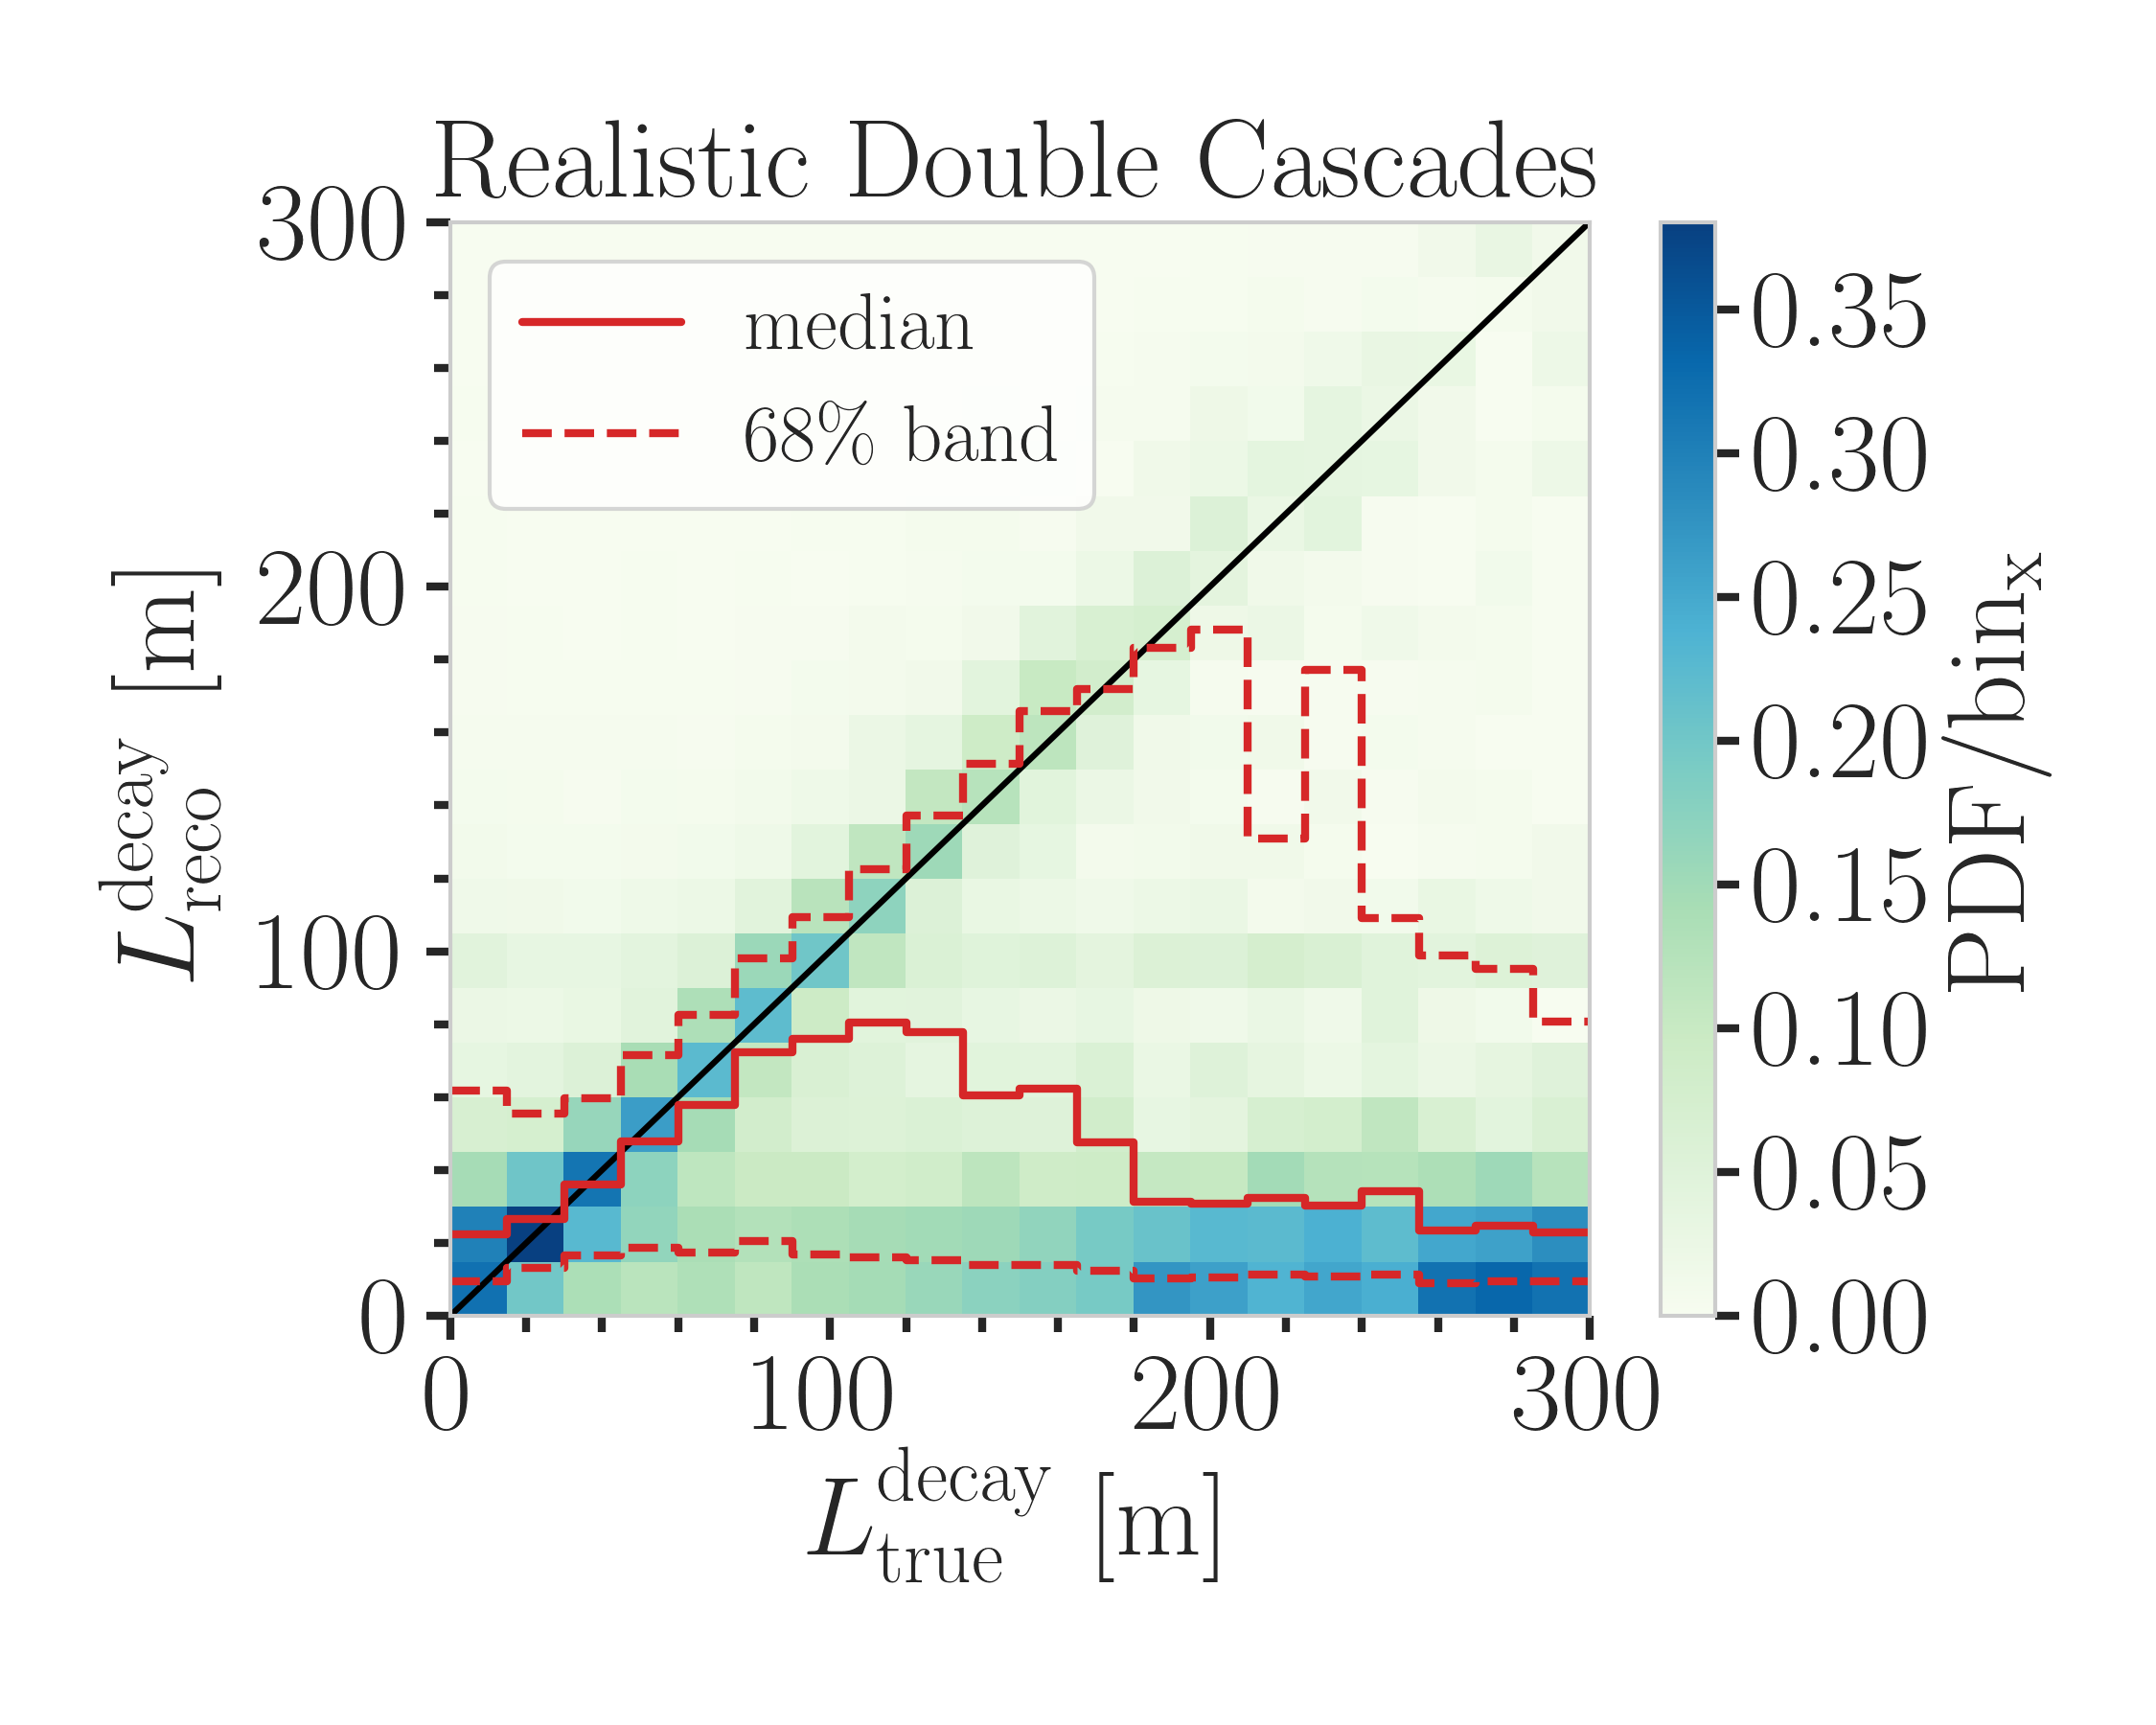
\includegraphics[width=0.49\linewidth]{figures/model_independent_simulation/results/realistic/2d_hists/194603_reco_decay_length_vs_true_decay_length_goodfit_step_contours.png}
    \caption[]{}
    \labfig{total_energy_decay_length_2dhists}
\end{figure*}
\todo{fix caption of this figure (RED)}

\begin{figure*}[h]
	\centering
    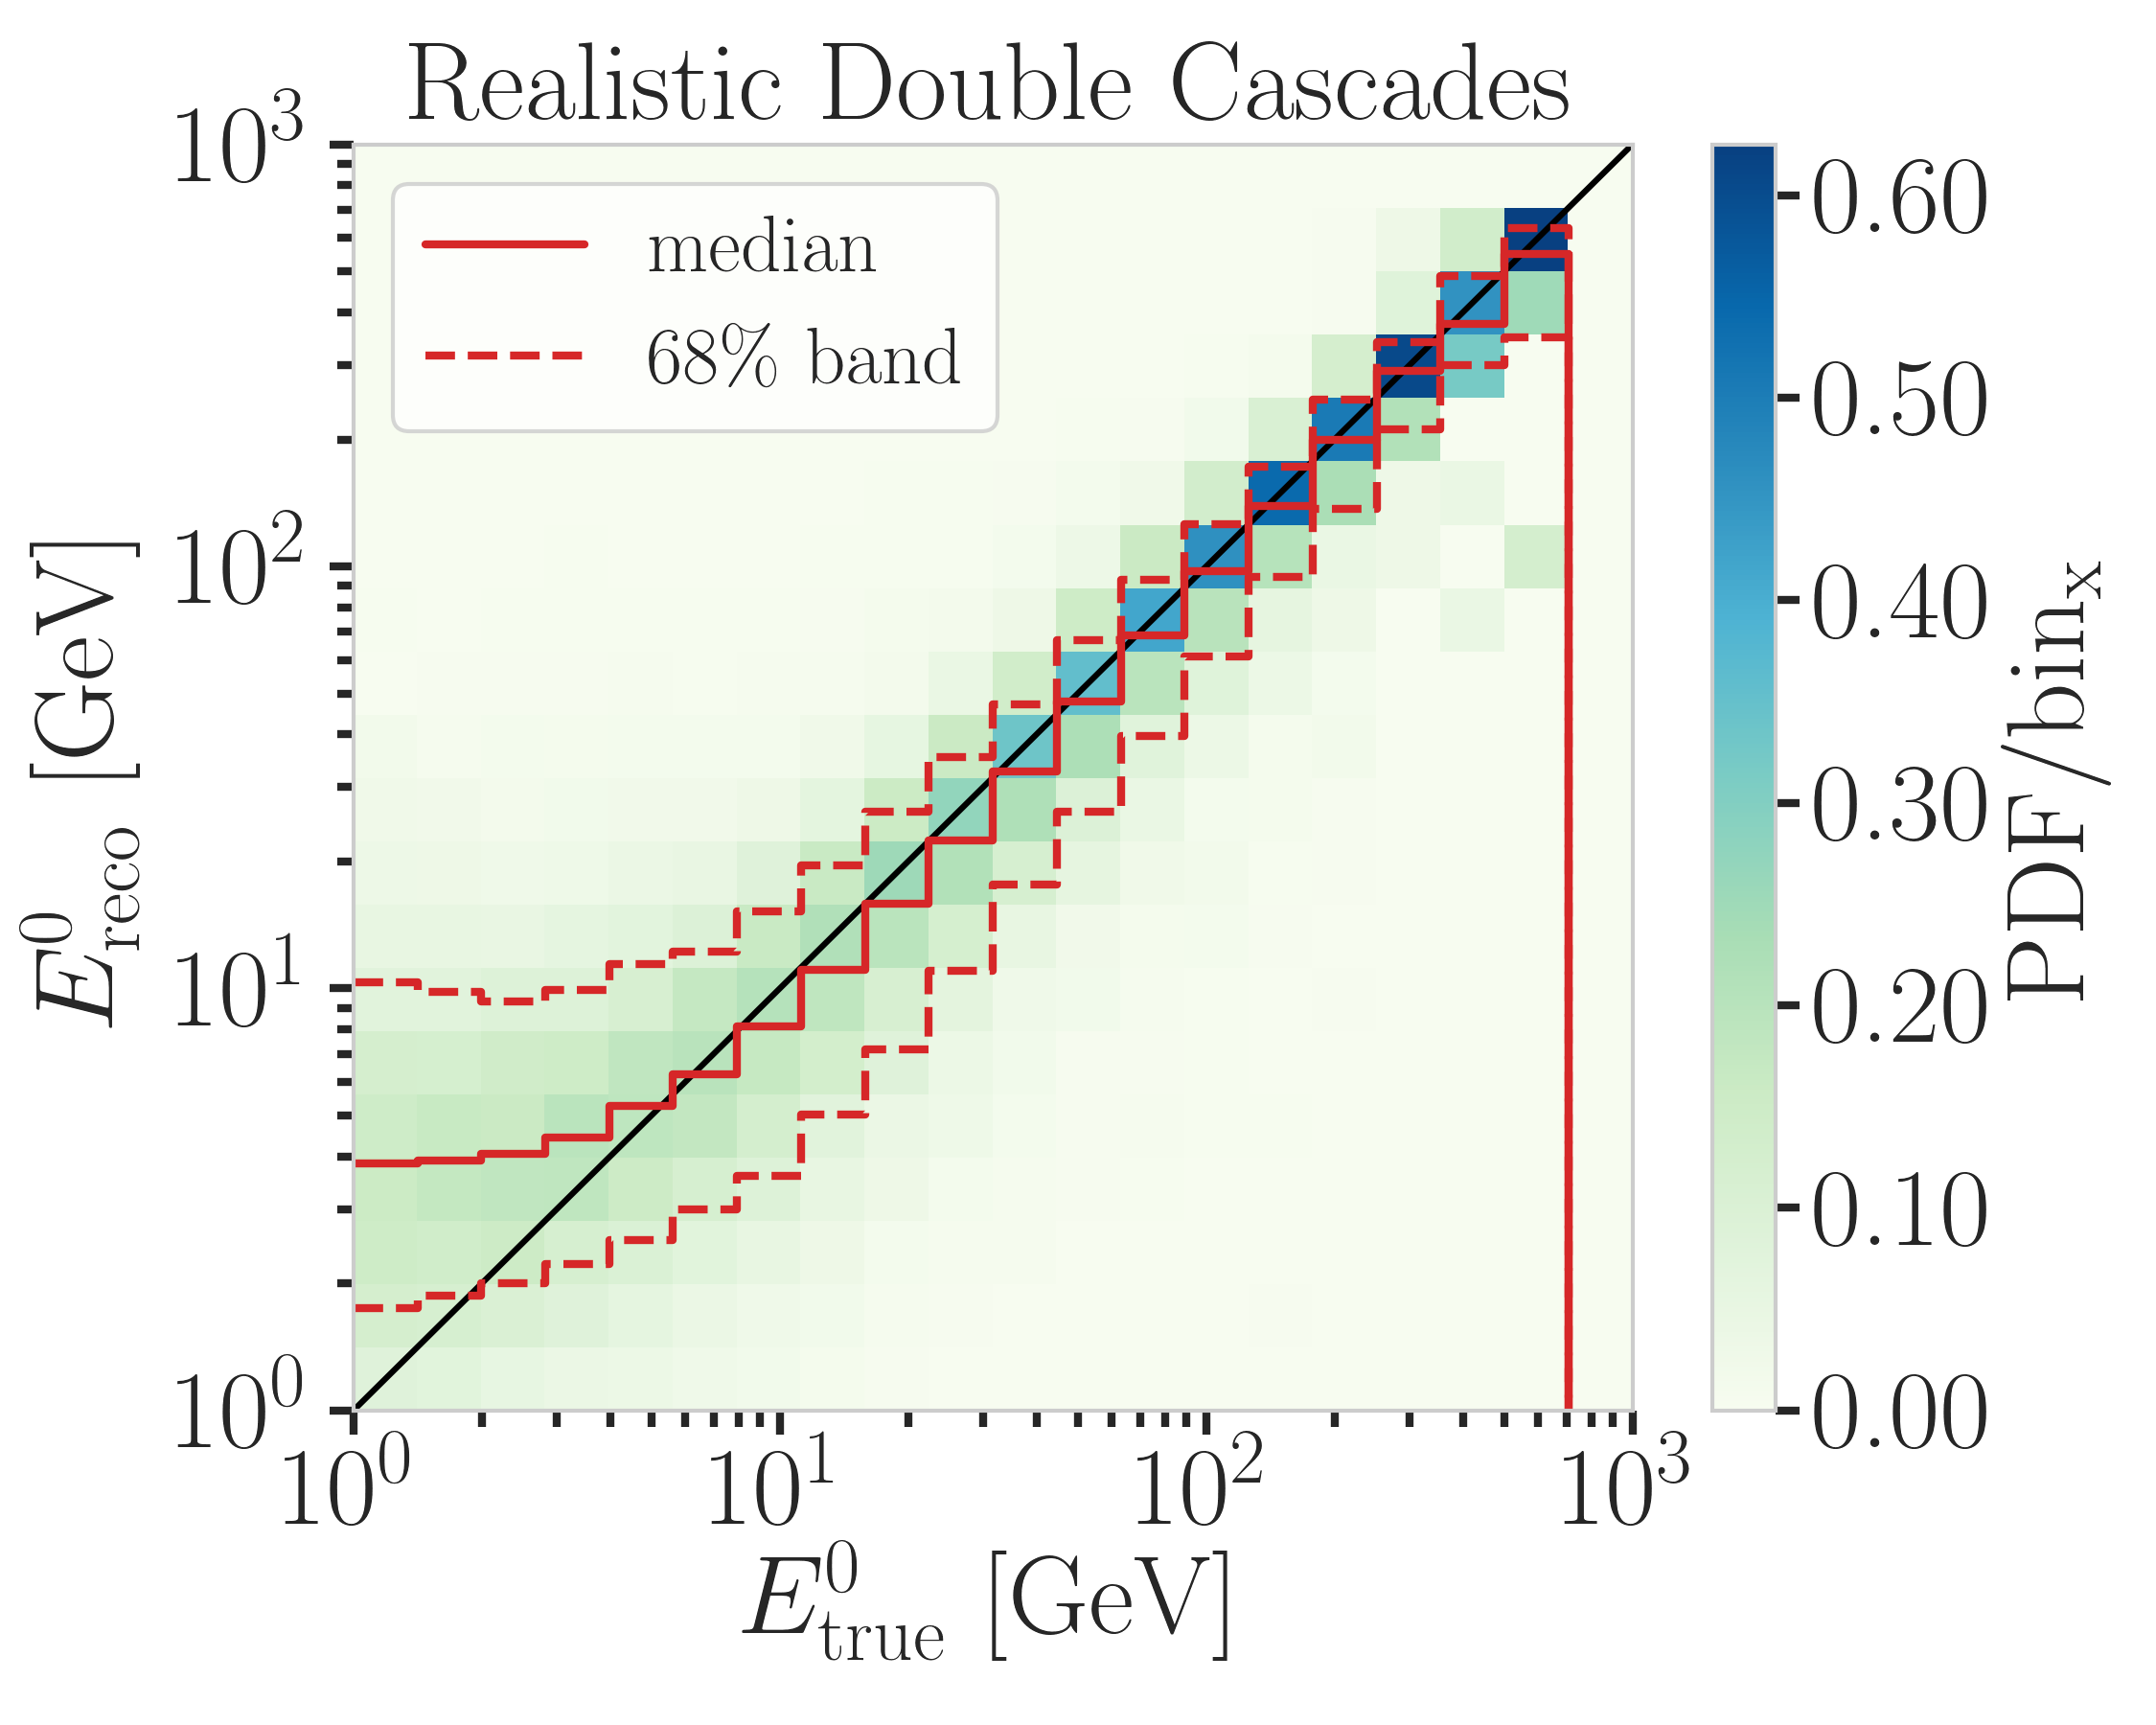
\includegraphics[width=0.49\linewidth]{figures/model_independent_simulation/results/realistic/2d_hists/194603_casc0_reco_energy_vs_casc0_true_energy_goodfit_step_contours.png}
    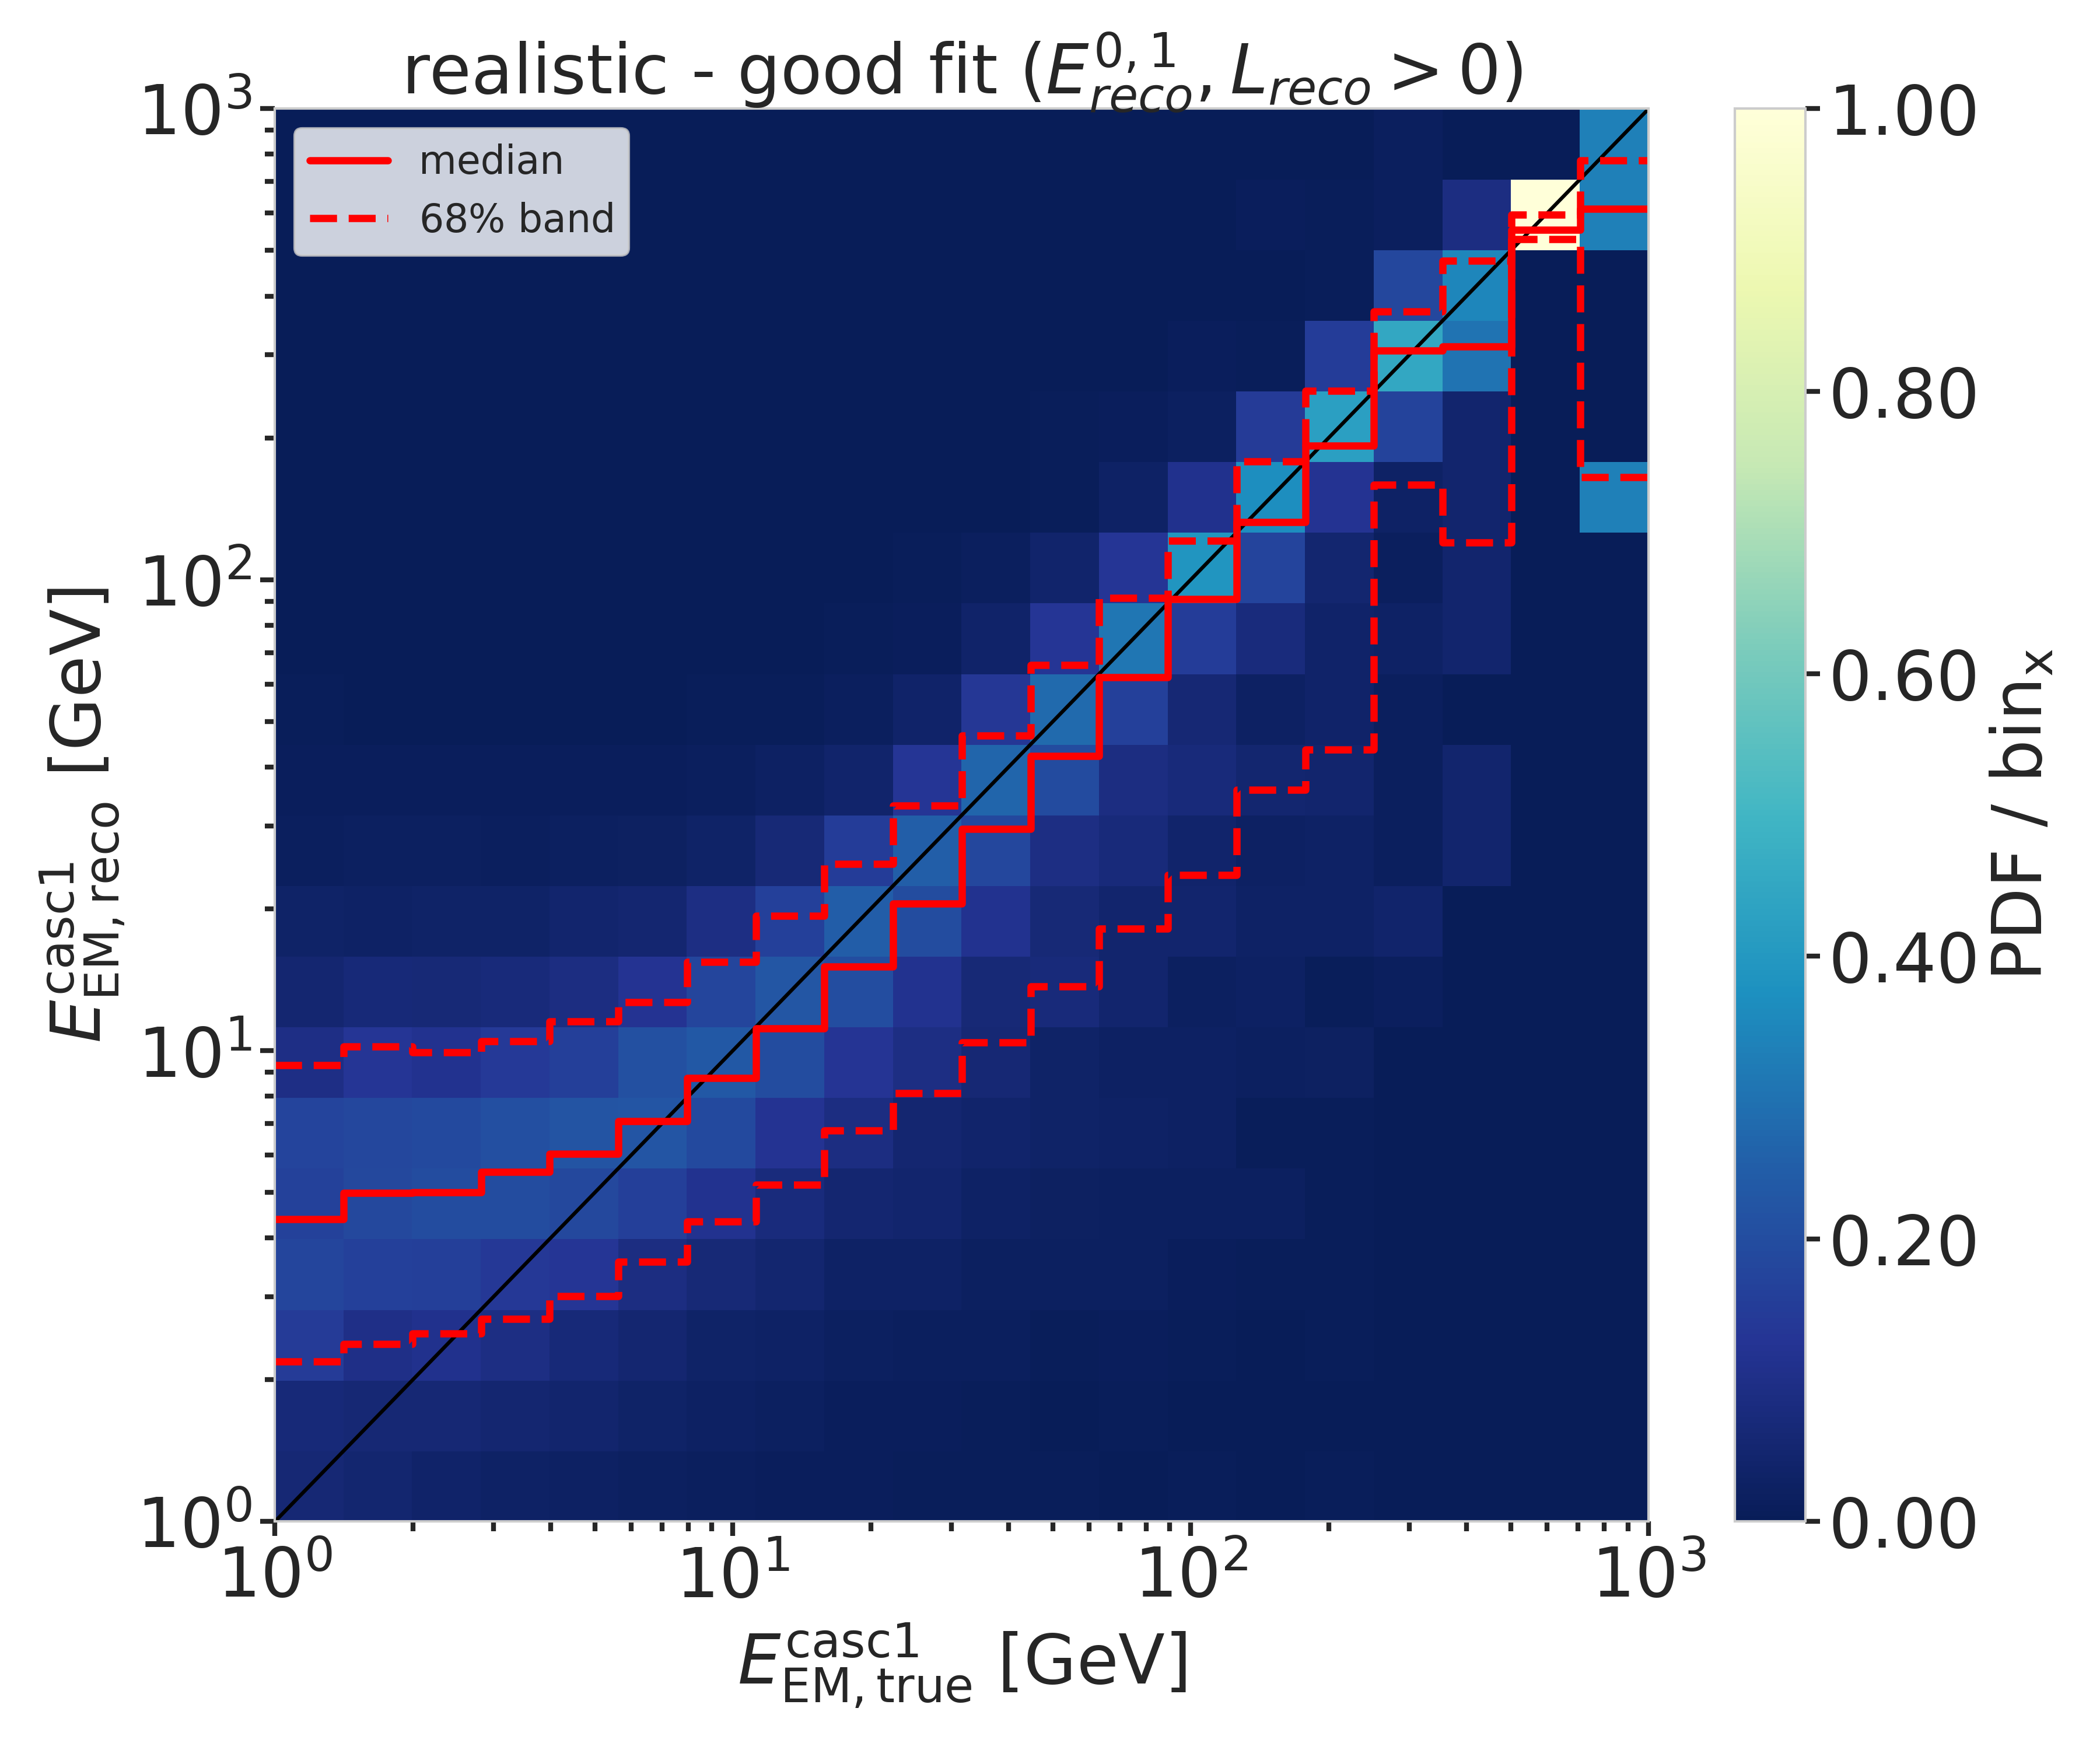
\includegraphics[width=0.49\linewidth]{figures/model_independent_simulation/results/realistic/2d_hists/194603_casc1_reco_energy_vs_casc1_true_energy_goodfit_step_contours.png}
    \caption[]{}
    \labfig{cascade_energy_2dhists}
\end{figure*}
\todo{fix caption of this figure (RED)}


\paragraph{Energy Resolution}

\textbf{Things to mention about the energy resolution:}
\begin{itemize}
    \item Here it can be seen more clearly how the median total energy resolution starts to stabilize around 0.0 at \SI{10}{\gev}, while for lower energies the reconstruction is over-estimating the true energy. This is a known behavior of energy reconstructions in IceCube, which is mainly due to a selection effect. Only events with a certain amount of light can be reconstructed, which means that the ones with true small energies that are still in the sample are events with over average light production due to fluctuations or other effects?
\end{itemize}

\begin{figure}[h]
	\centering
    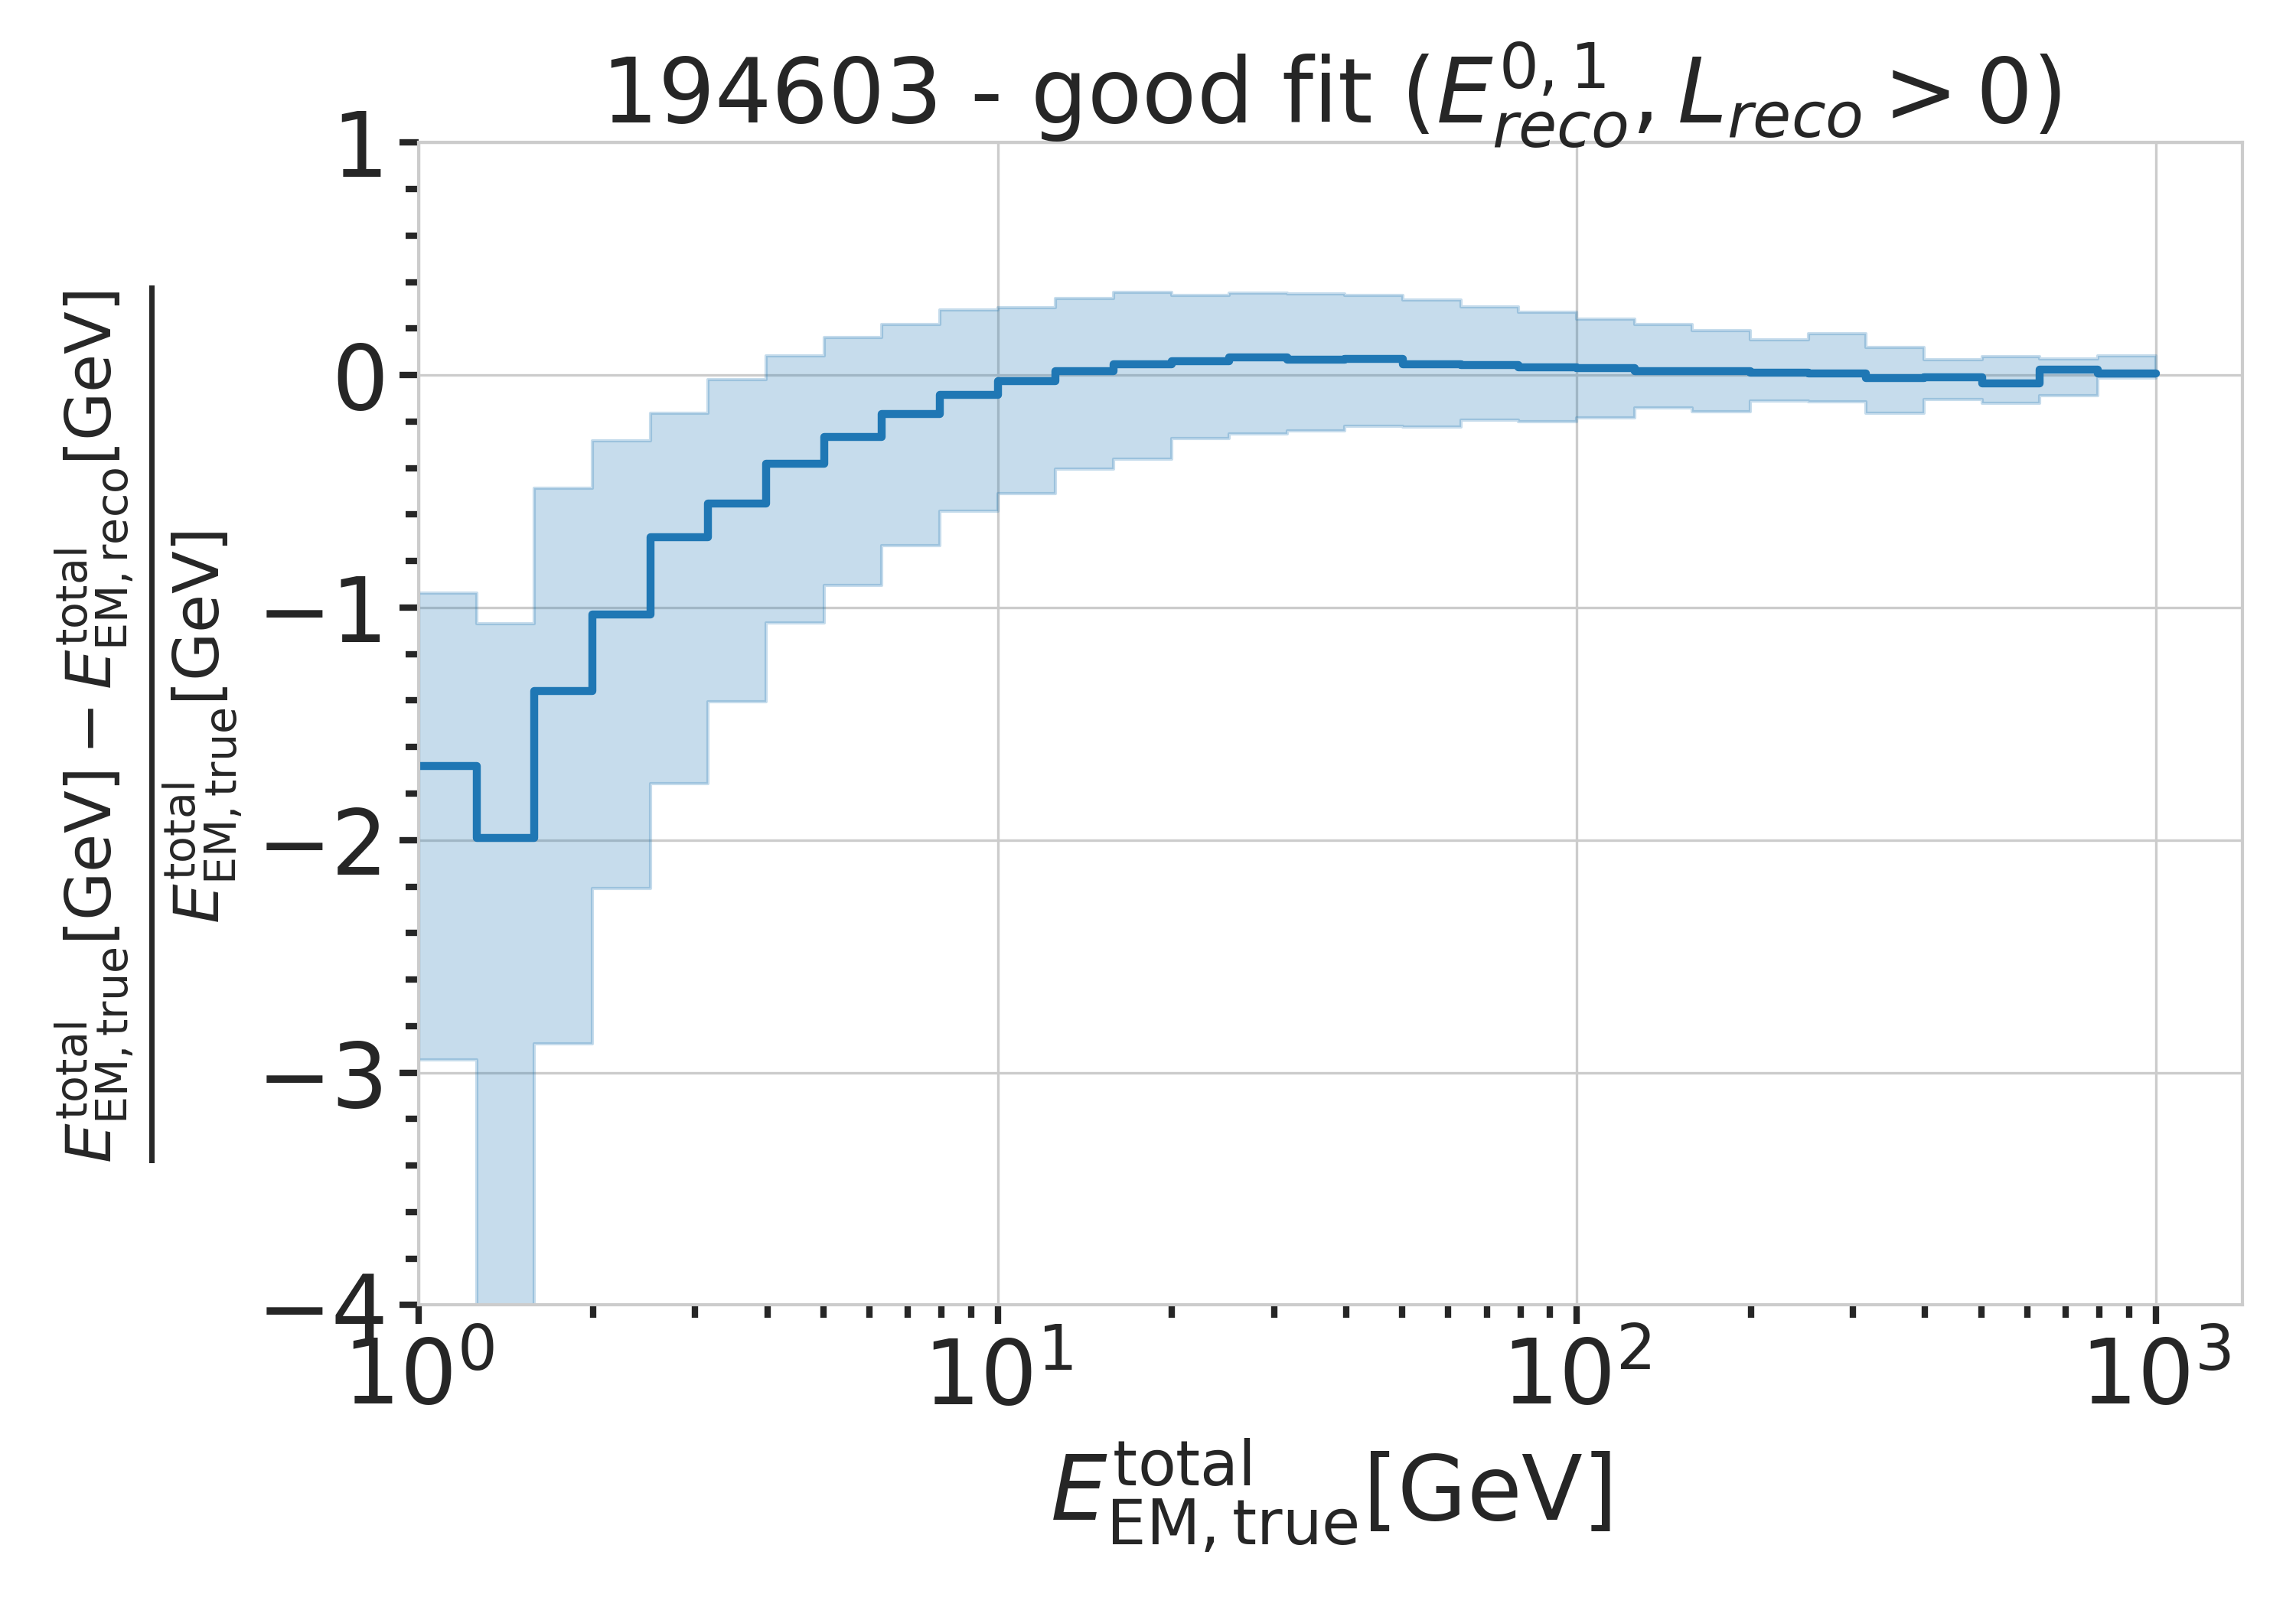
\includegraphics{figures/model_independent_simulation/results/realistic/resolutions/194603_fractional_reco_total_energy_error_goodfit.png}
    \caption[]{}
    \labfig{total_energy_bias_vs_energy}
\end{figure}
\todo{fix caption of this figure (RED)}


\paragraph{Decay Length Resolution}

\textbf{Things to mention about the decay length resolution:}
\begin{itemize}
    \item As already mentioned before, the decay length resolution is much worse than the energy resolutions. \reffig{decay_length_bias_vs_length} also shows that the median is below 0.0 for short true length and above 0.0 and approaching 1.0 for long true lengths.
    \item To investigate whether this is really due to the fact that one of the cascades is not observed, the decay length resolution was plotted against the total energy of the event and the minimum energy of the two cascades \reffig{decay_length_bias_vs_energies}.
    \item It can be seen that the median of the decay length resolution stabilizes at 0.0 for a total energy above \SI{20}{\gev}, but the spread of the distribution is still quite large with a 1-sigma band of \SIrange{80}{100}{\percent}.
    \item From the plot against the minimum energy it can be seen that the decay length resolution starts to be unbiased for a minimum energy of the cascades of \SI{7}{\gev}, with an equivalently large spread.
    \item A preliminary takeaway from this is that the decay length reconstruction is not reliable at all for events with a total energy below \SI{20}{\gev} or a minimum cascade energy below \SI{7}{\gev}.
\end{itemize}

\begin{figure}[h]
	\centering
    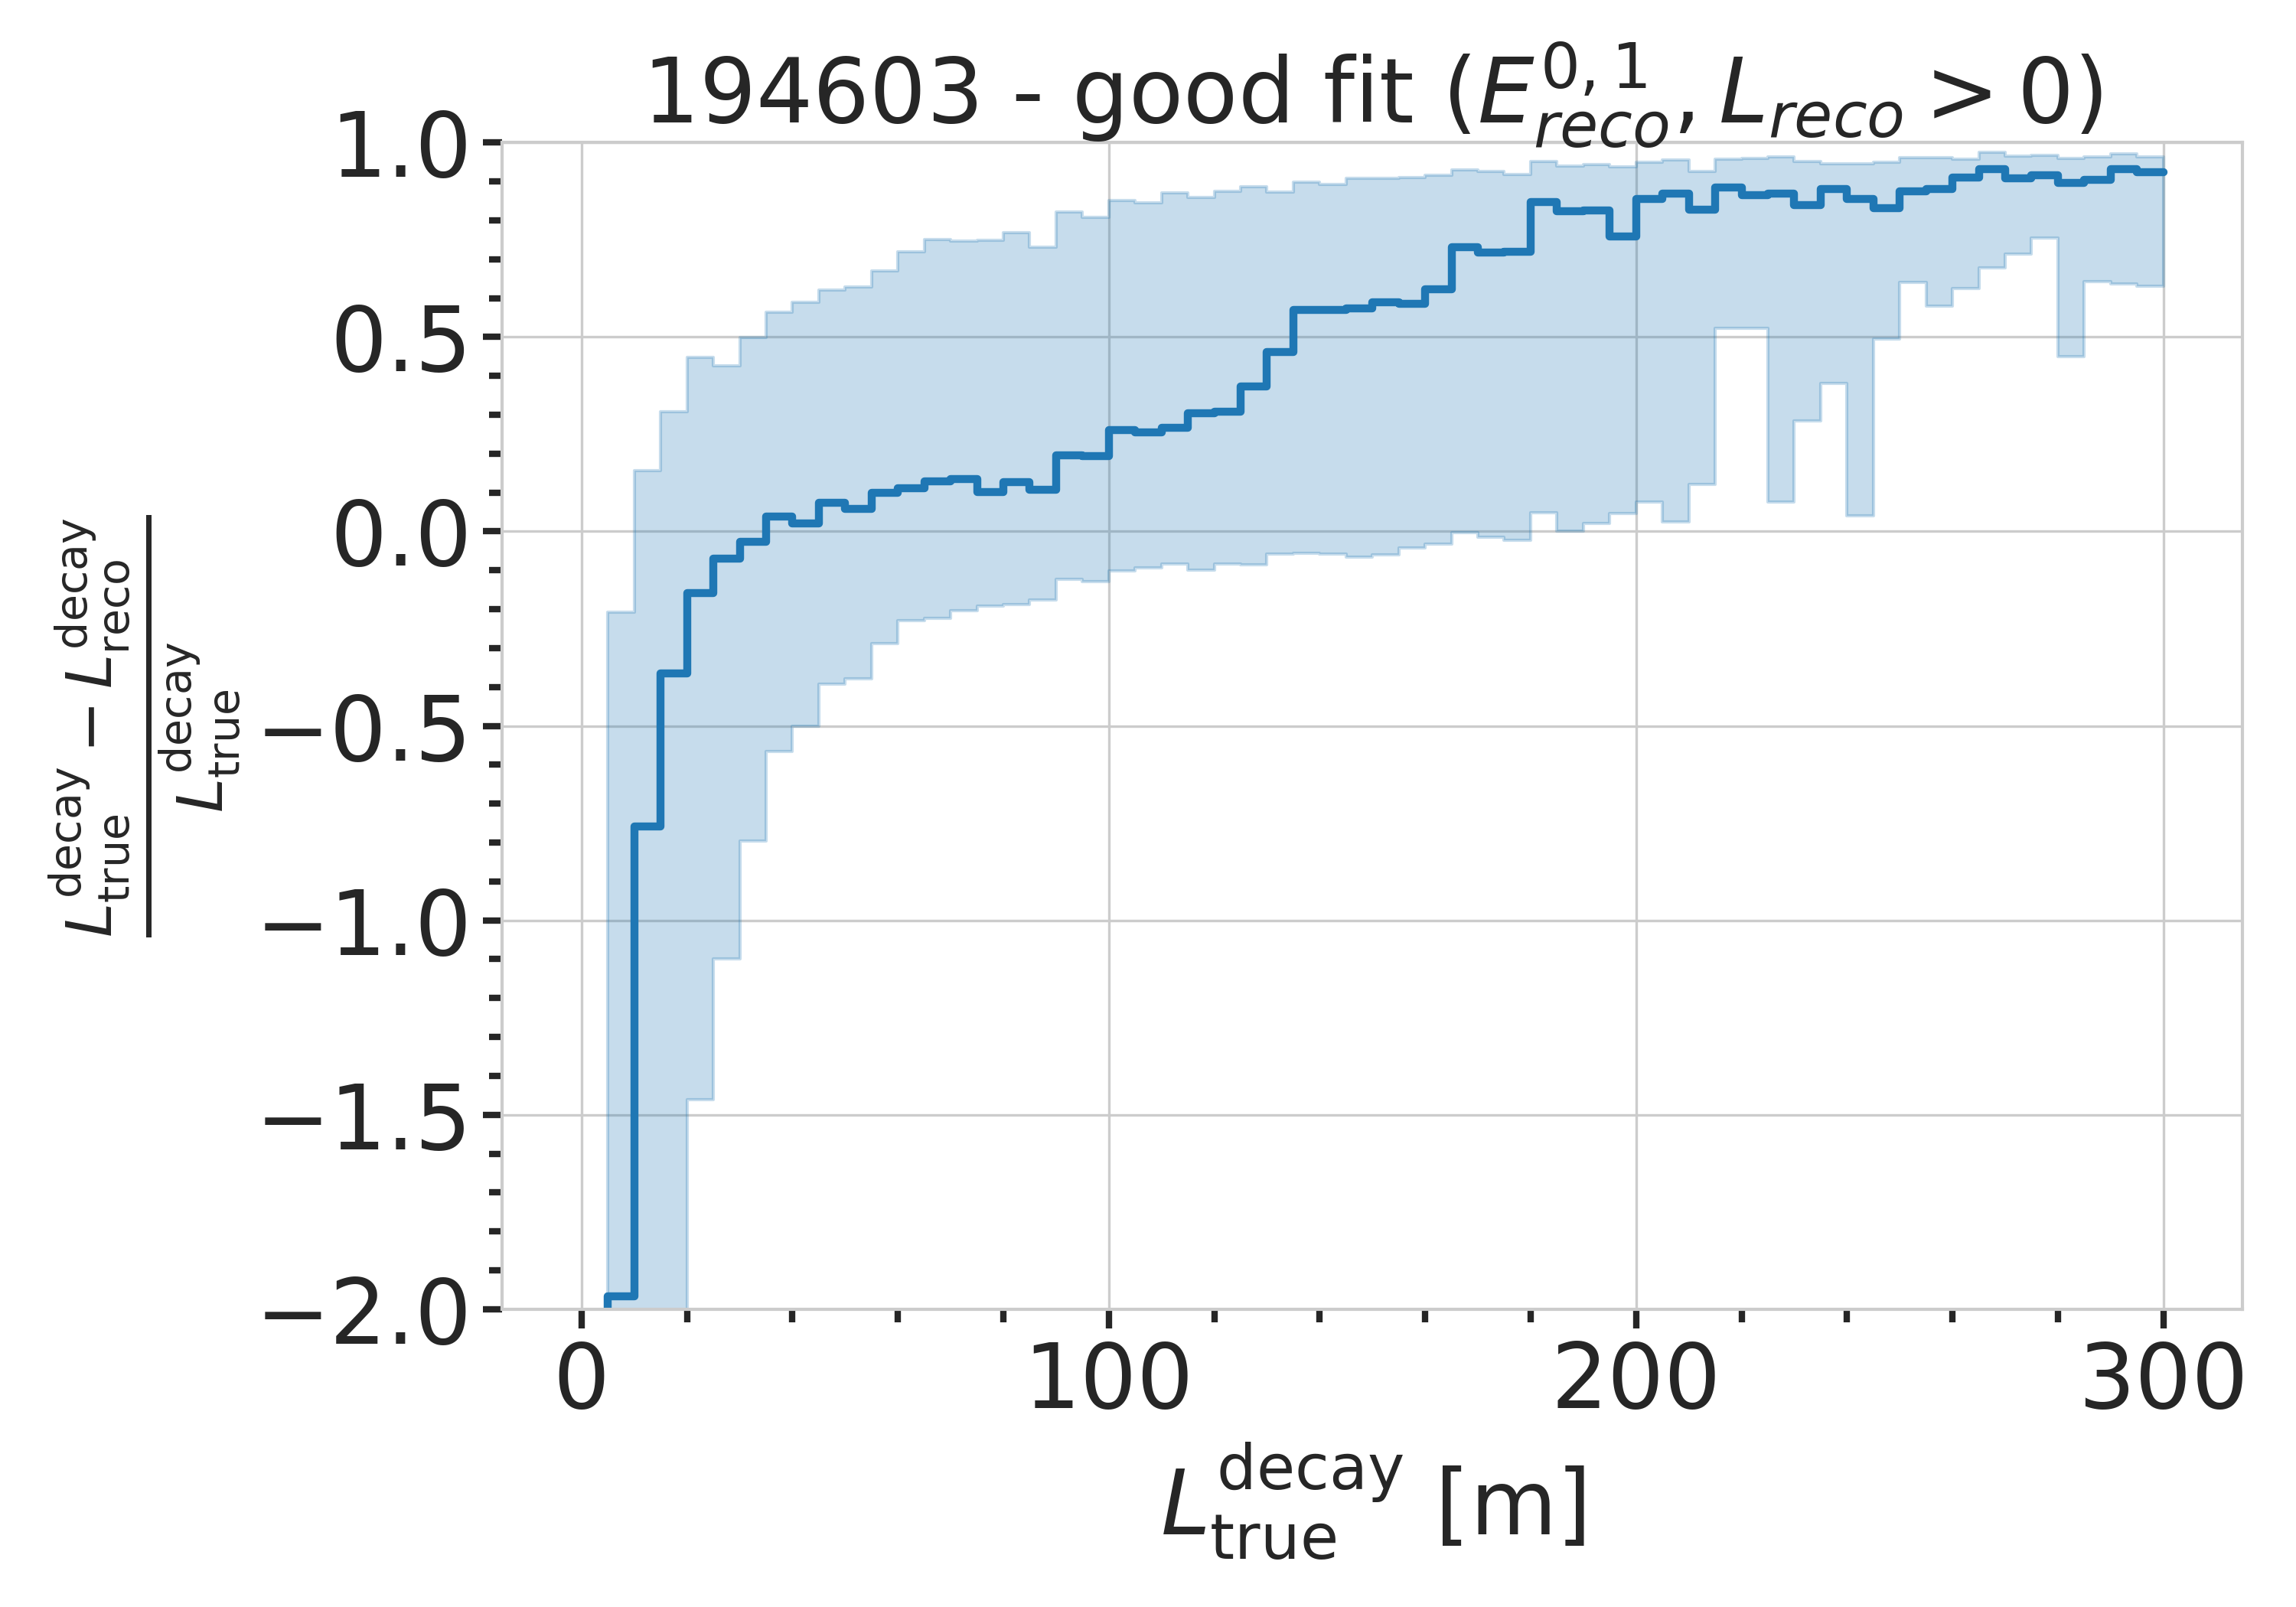
\includegraphics{figures/model_independent_simulation/results/realistic/resolutions/194603_median_decay_length_bias_goodfit_log_unweighted.png}
    \caption[]{}
    \labfig{decay_length_bias_vs_length}
\end{figure}
\todo{fix caption of this figure (RED)}


\begin{figure*}[h]
	\centering
    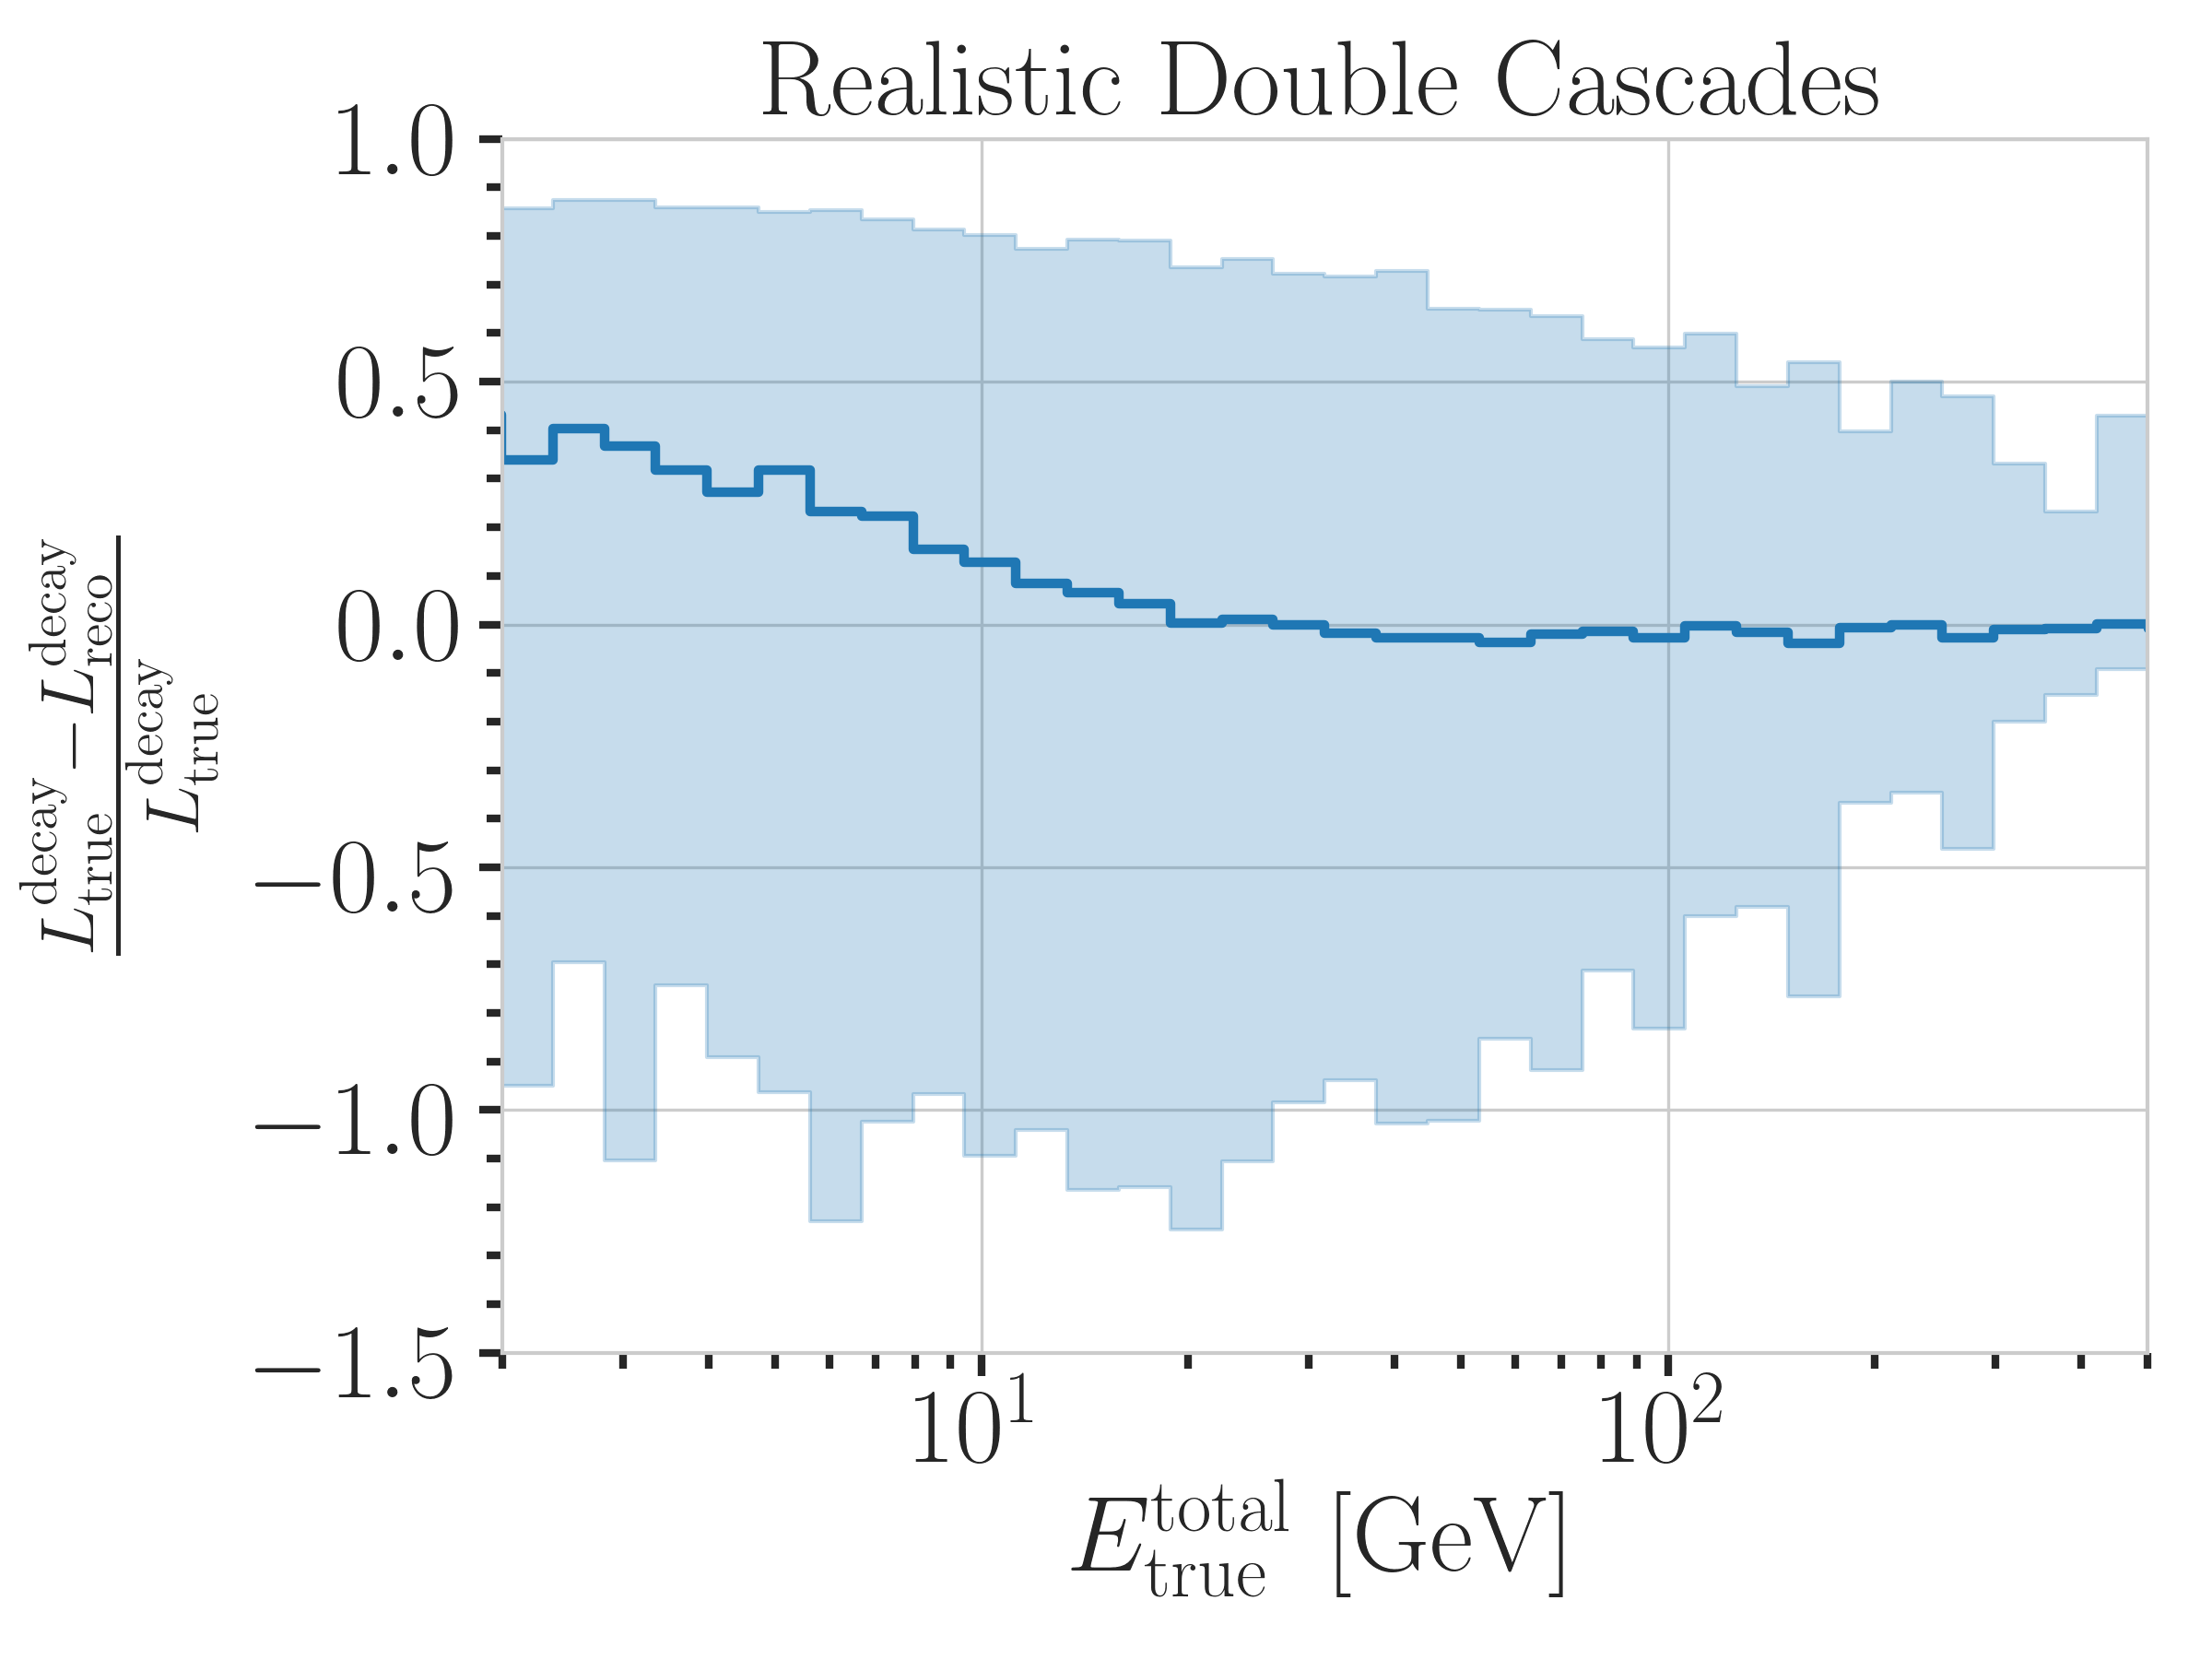
\includegraphics[width=0.49\linewidth]{figures/model_independent_simulation/results/realistic/resolutions/194603_median_decay_length_bias_vs_tot_energy_goodfit_log_unweighted.png}
    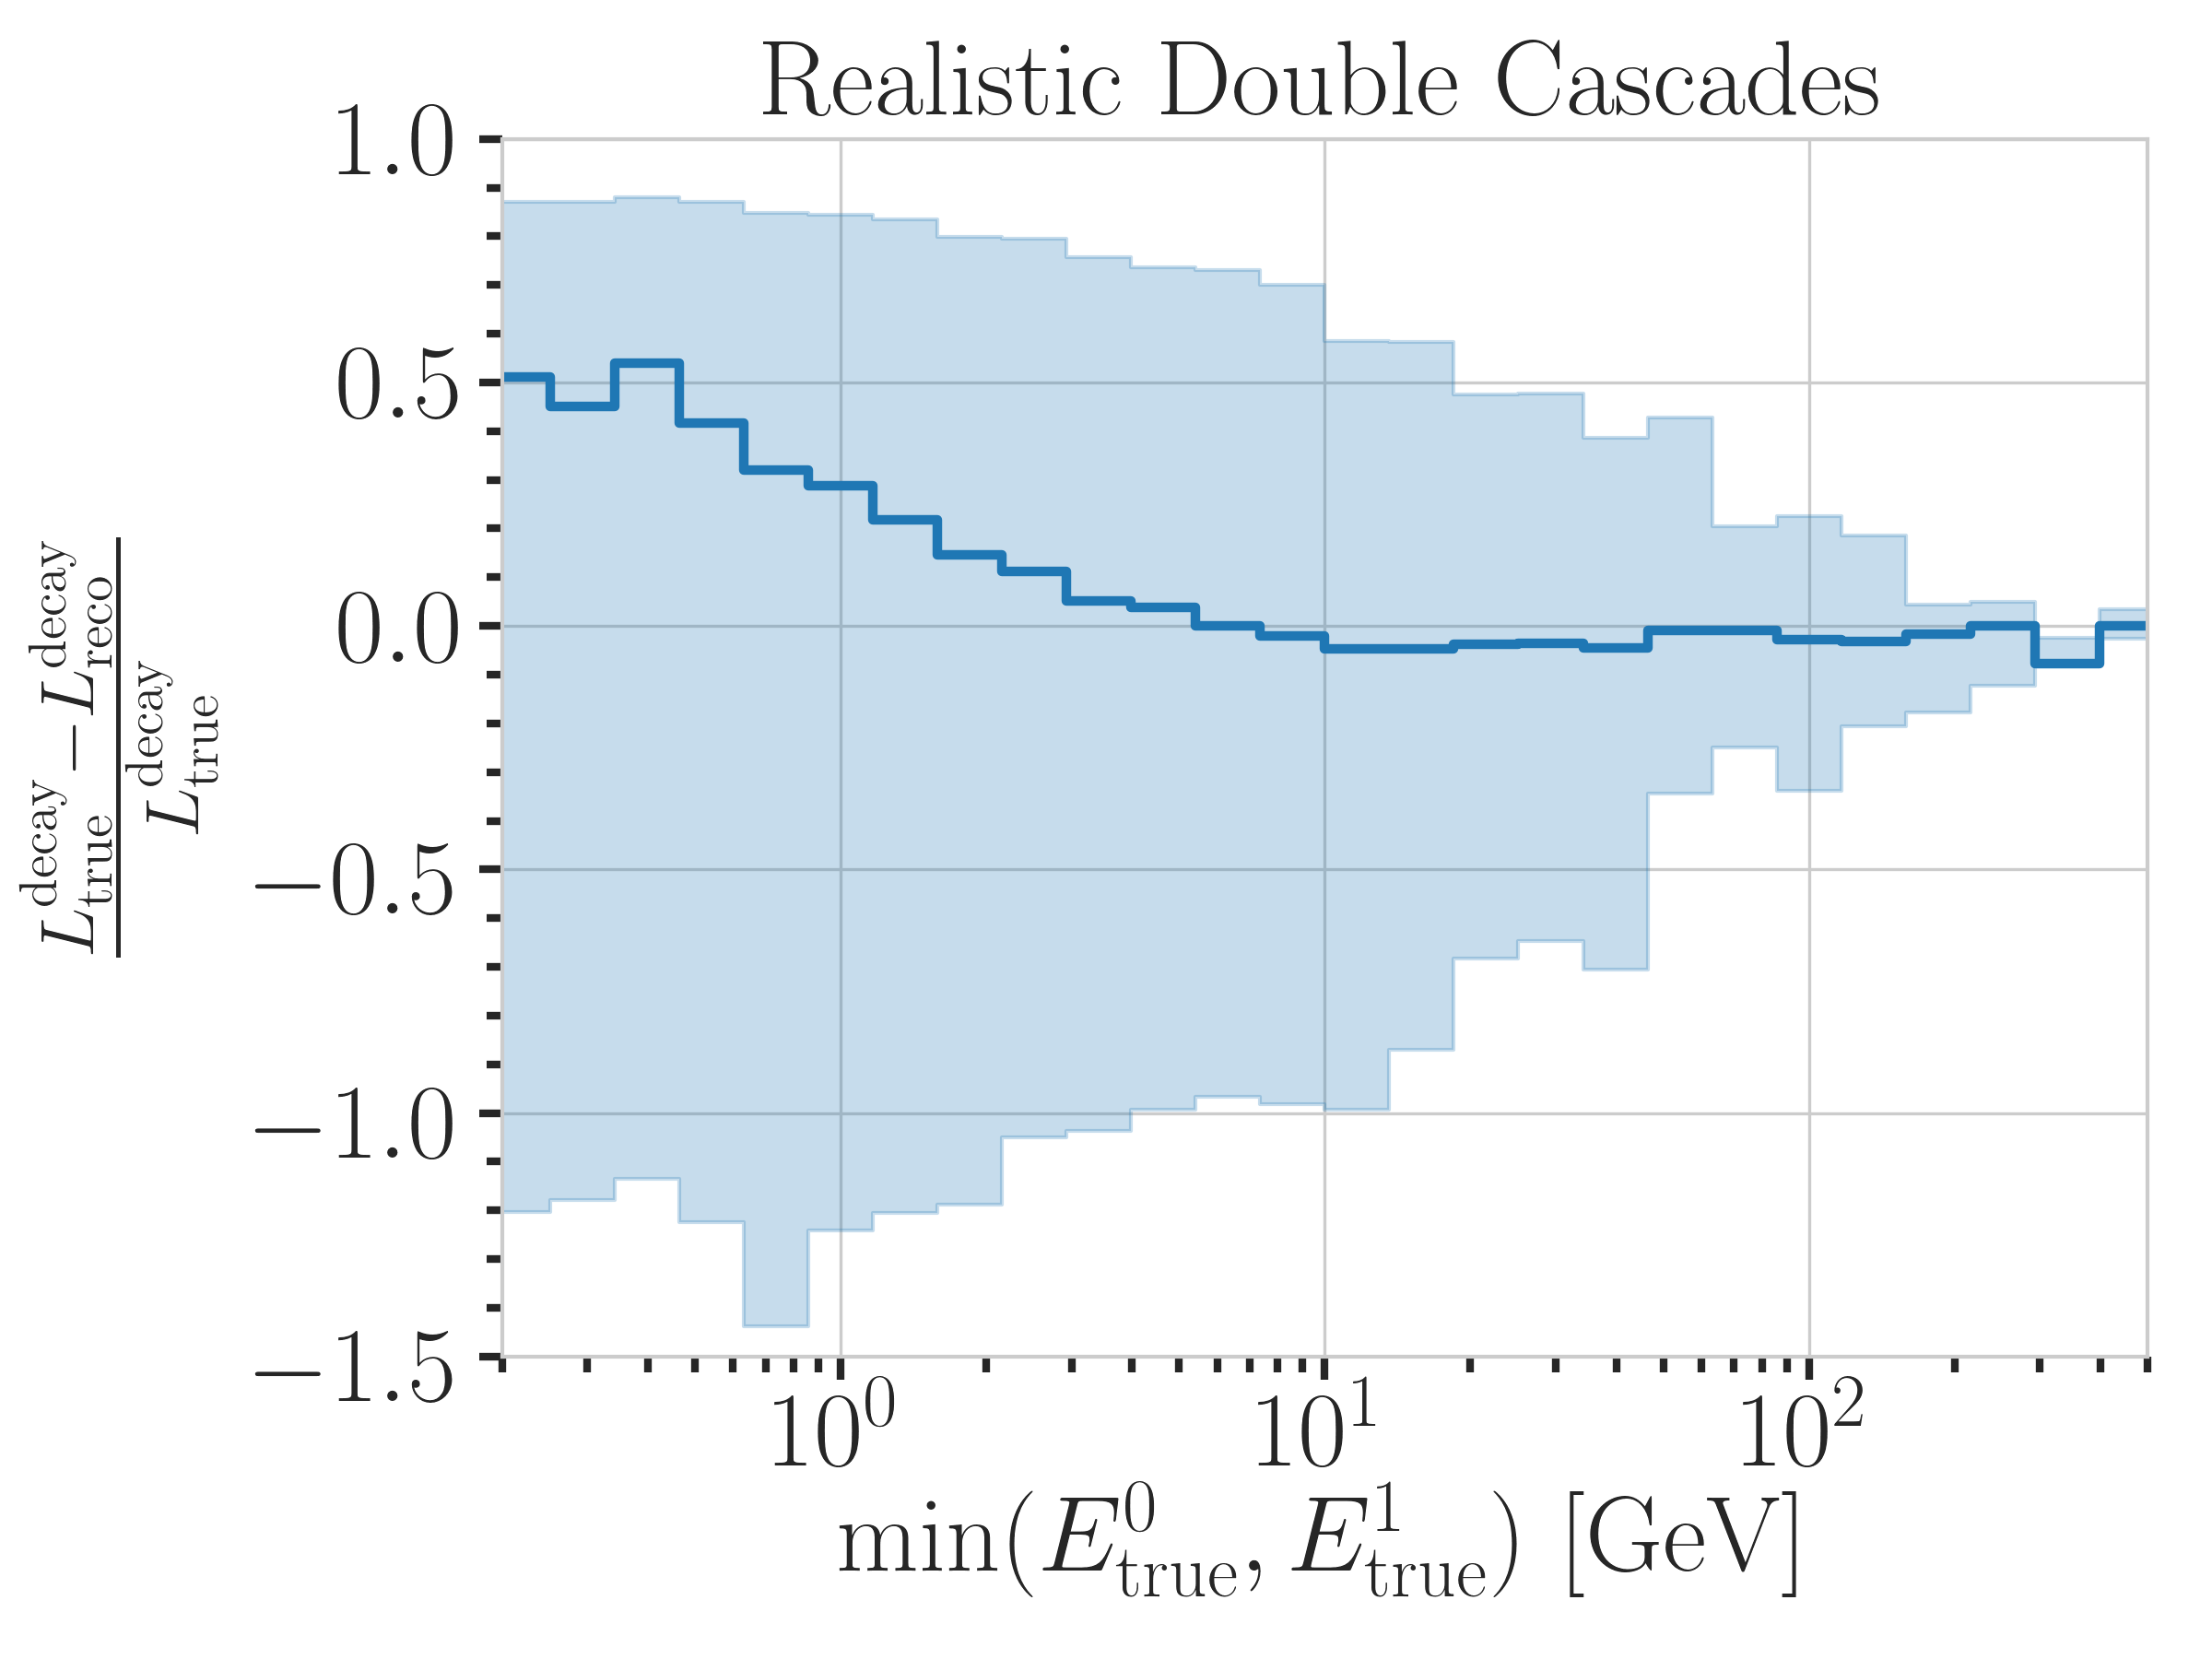
\includegraphics[width=0.49\linewidth]{figures/model_independent_simulation/results/realistic/resolutions/194603_median_decay_length_bias_vs_min_energy_goodfit_log_unweighted.png} 
    \caption[]{}
    \labfig{decay_length_bias_vs_energies}
\end{figure*}
\todo{fix caption of this figure (RED)}


\subsection{Low Energy Event Selection Efficiency}

\todo{Make plot to show efficiency of the OscNext selection for HNL events. (ORANGE)}

\paragraph{Discussion ideas:}
\begin{itemize}
    \item Show energy, length distribution across the different levels?
    \item Show efficiency as table across the different levels (MC events + fraction?)
    \item Compare this to BG efficiency? (maybe rather for the discussion)
    \item At which level does the selection reduce the HNL the most?
    \item Is there a place to improve the HNL selection? (Might have to factor in the BG efficiency, as well..)
    \item What of this might change with Upgrade? (maybe rather for the discussion)
\end{itemize}
